\chapter{The tool}

\section{General description}
\label{tool_general_description}
The tool has two components: a \textit{data gatherer} and a \textit{visualization client}.

The data gatherer is a C++ header-only class of which methods have to be called within the main loop of any unidirectional path tracer. It stores to disk data generated --- and usually discarded --- by the path tracer during rendering. For each path shoot by the renderer the tool stores its transported radiance, its camera sample, and the world positions of its bounces. 

Once the rendering is done and the data is collected, the visualization client can be used to explore the gathered information. To allow interactive 3D exploration it also needs a scene description; this is not generated by the gatherer and it has to be provided separately by the user. The scene format used is novel, based on triangle meshes and it shares many similarities with glTF \cite{robinet2014gltf}. This peculiar choice has been done mainly to not do any assumptions on the kind of geometry representation the path tracer uses. In this way even path tracers that use exotic geometries can be analyzed with the tool --- at least until the user is able to convert whatever they are using in triangles.

\section{Technology}
\label{technology}

Before talking about the actual implementations, here is presented a summary of the technologies used to create the tool.

The data gatherer has been developed as a header-only C++17\footnote{C++17 is the informal name of the ISO/IEC 14882:2017 standard. \url{https://www.iso.org/standard/68564.html}} library. The choice was motivated by the belief --- not backed by any data --- that most path tracers, included the ones written by students, are written in C++. In hindsight, probably writing it in pure C would have made it potentially compatible with more path tracers; after all it uses very few features of C++. 

Deciding the technologies to use for the visualization client took more careful thinking, since it was clear it would be the biggest software piece in the context of this project. The final combination consists in:
\begin{description}
	\item[C++] Due to the available expertise, the other plausible languages were Python and --- for a very brief moment --- Julia, but they were discarded due to the necessity of managing memory and threads directly. C has been considered too, but STL and OOP made the scale tip over C++. As for the data gatherer, C++17 is used.
	\item[“Raw” OpenGL] Rendering hundreds of thousands paths in an interactive and fully customizable fashion was perceived since the beginning as no easy task and it made clear the necessity to be able to control and program every possible stage of the rendering pipeline. Due to this, visualization frameworks such as VTK \cite{vtk2006} had been ruled out immediately in favor of just GLEW and GLFW3 to provide an OpenGL 4.6 Core Profile context.
	\item[Dear ImGui] Since all rendering customization needs came from the interactive 3d rendering of paths and scenes, using just OpenGL to build a GUI from scratch would have been insane and so a GUI framework had to be chosen. The final candidates were Qt5 and Dear ImGui\footnote{\url{https://github.com/ocornut/imgui}} but since ImGui was not completely familiar to the author, it has been chosen due to educational purposes.
	\item[Boost Log and Filesystem] It seemed like a good idea to have a complete logger and a filesystem library with a STL-like style and it led to the adoption of the Boost Log\footnote{\url{https://www.boost.org/doc/libs/1_75_0/libs/log/doc/html/index.html}} and Boost Filesystem\footnote{\url{https://www.boost.org/doc/libs/1_39_0/libs/filesystem/doc/index.htm}} libraries. Since it is not a crucial dependency, it might be removed in a future development.
\end{description}

Both the gatherer and the visualization client use a header-only math library called \textit{math.hpp}\footnote{\url{https://github.com/giuliom95/math}} to handle vector and matrix types and operations. It includes the \textit{half} library\footnote{\url{http://half.sourceforge.net/}} which is an implementation of the 16 bits floating point number representation, commonly called half precision float or just \texttt{half}, as described by the IEEE 754 standard\footnote{\url{https://ieeexplore.ieee.org/document/8766229}}.

\section{Data gatherer}

\subsection{The data to gather}
\label{datatogather}
Until now, it has been said that the gatherer has to be able to store “the paths with some useful data”, but how does one store a path and what is useful data have not been defined yet. In the beginning, the focus was on just visualizing paths in an interactive scene rendering so that the user could see how paths interact with the scene. To achieve that it was clear the actual geometry of all paths had to be stored. This meant storing for each path a camera sample and all of its bounces.
Several ways of storing path bounces had been considered, such as storing each bounce as a direction and a distance, but the most na\"ive solution has been opted: each bounce is stored as a 3-dimensional point in world space.

This immediately raised some concerns about how much memory would be required to store all these points: let us calculate how many bytes it would take to just store the bounces of all paths needed to produce image \ref{hall_render}. It is 512 pixels wide and 512 pixels tall, it has been rendered with 512 samples per pixel --- spp --- each with a depth of maximum 10 --- this means that each of the 512 paths shoot every pixel bounced in the scene at most 10 times. Storing the points as a triplet of single precision float numbers --- 4 bytes, the C++ built-in \texttt{float} type ---  we would have:
\begin{equation}
	\label{rough_bounce_size_estimation}
	(512 \times 512) pixels \times 512 spp \times 10 bounces \times 3 dimensions \times 4 bytes \approx 15GB
\end{equation}
\begin{figure}
	\centering
	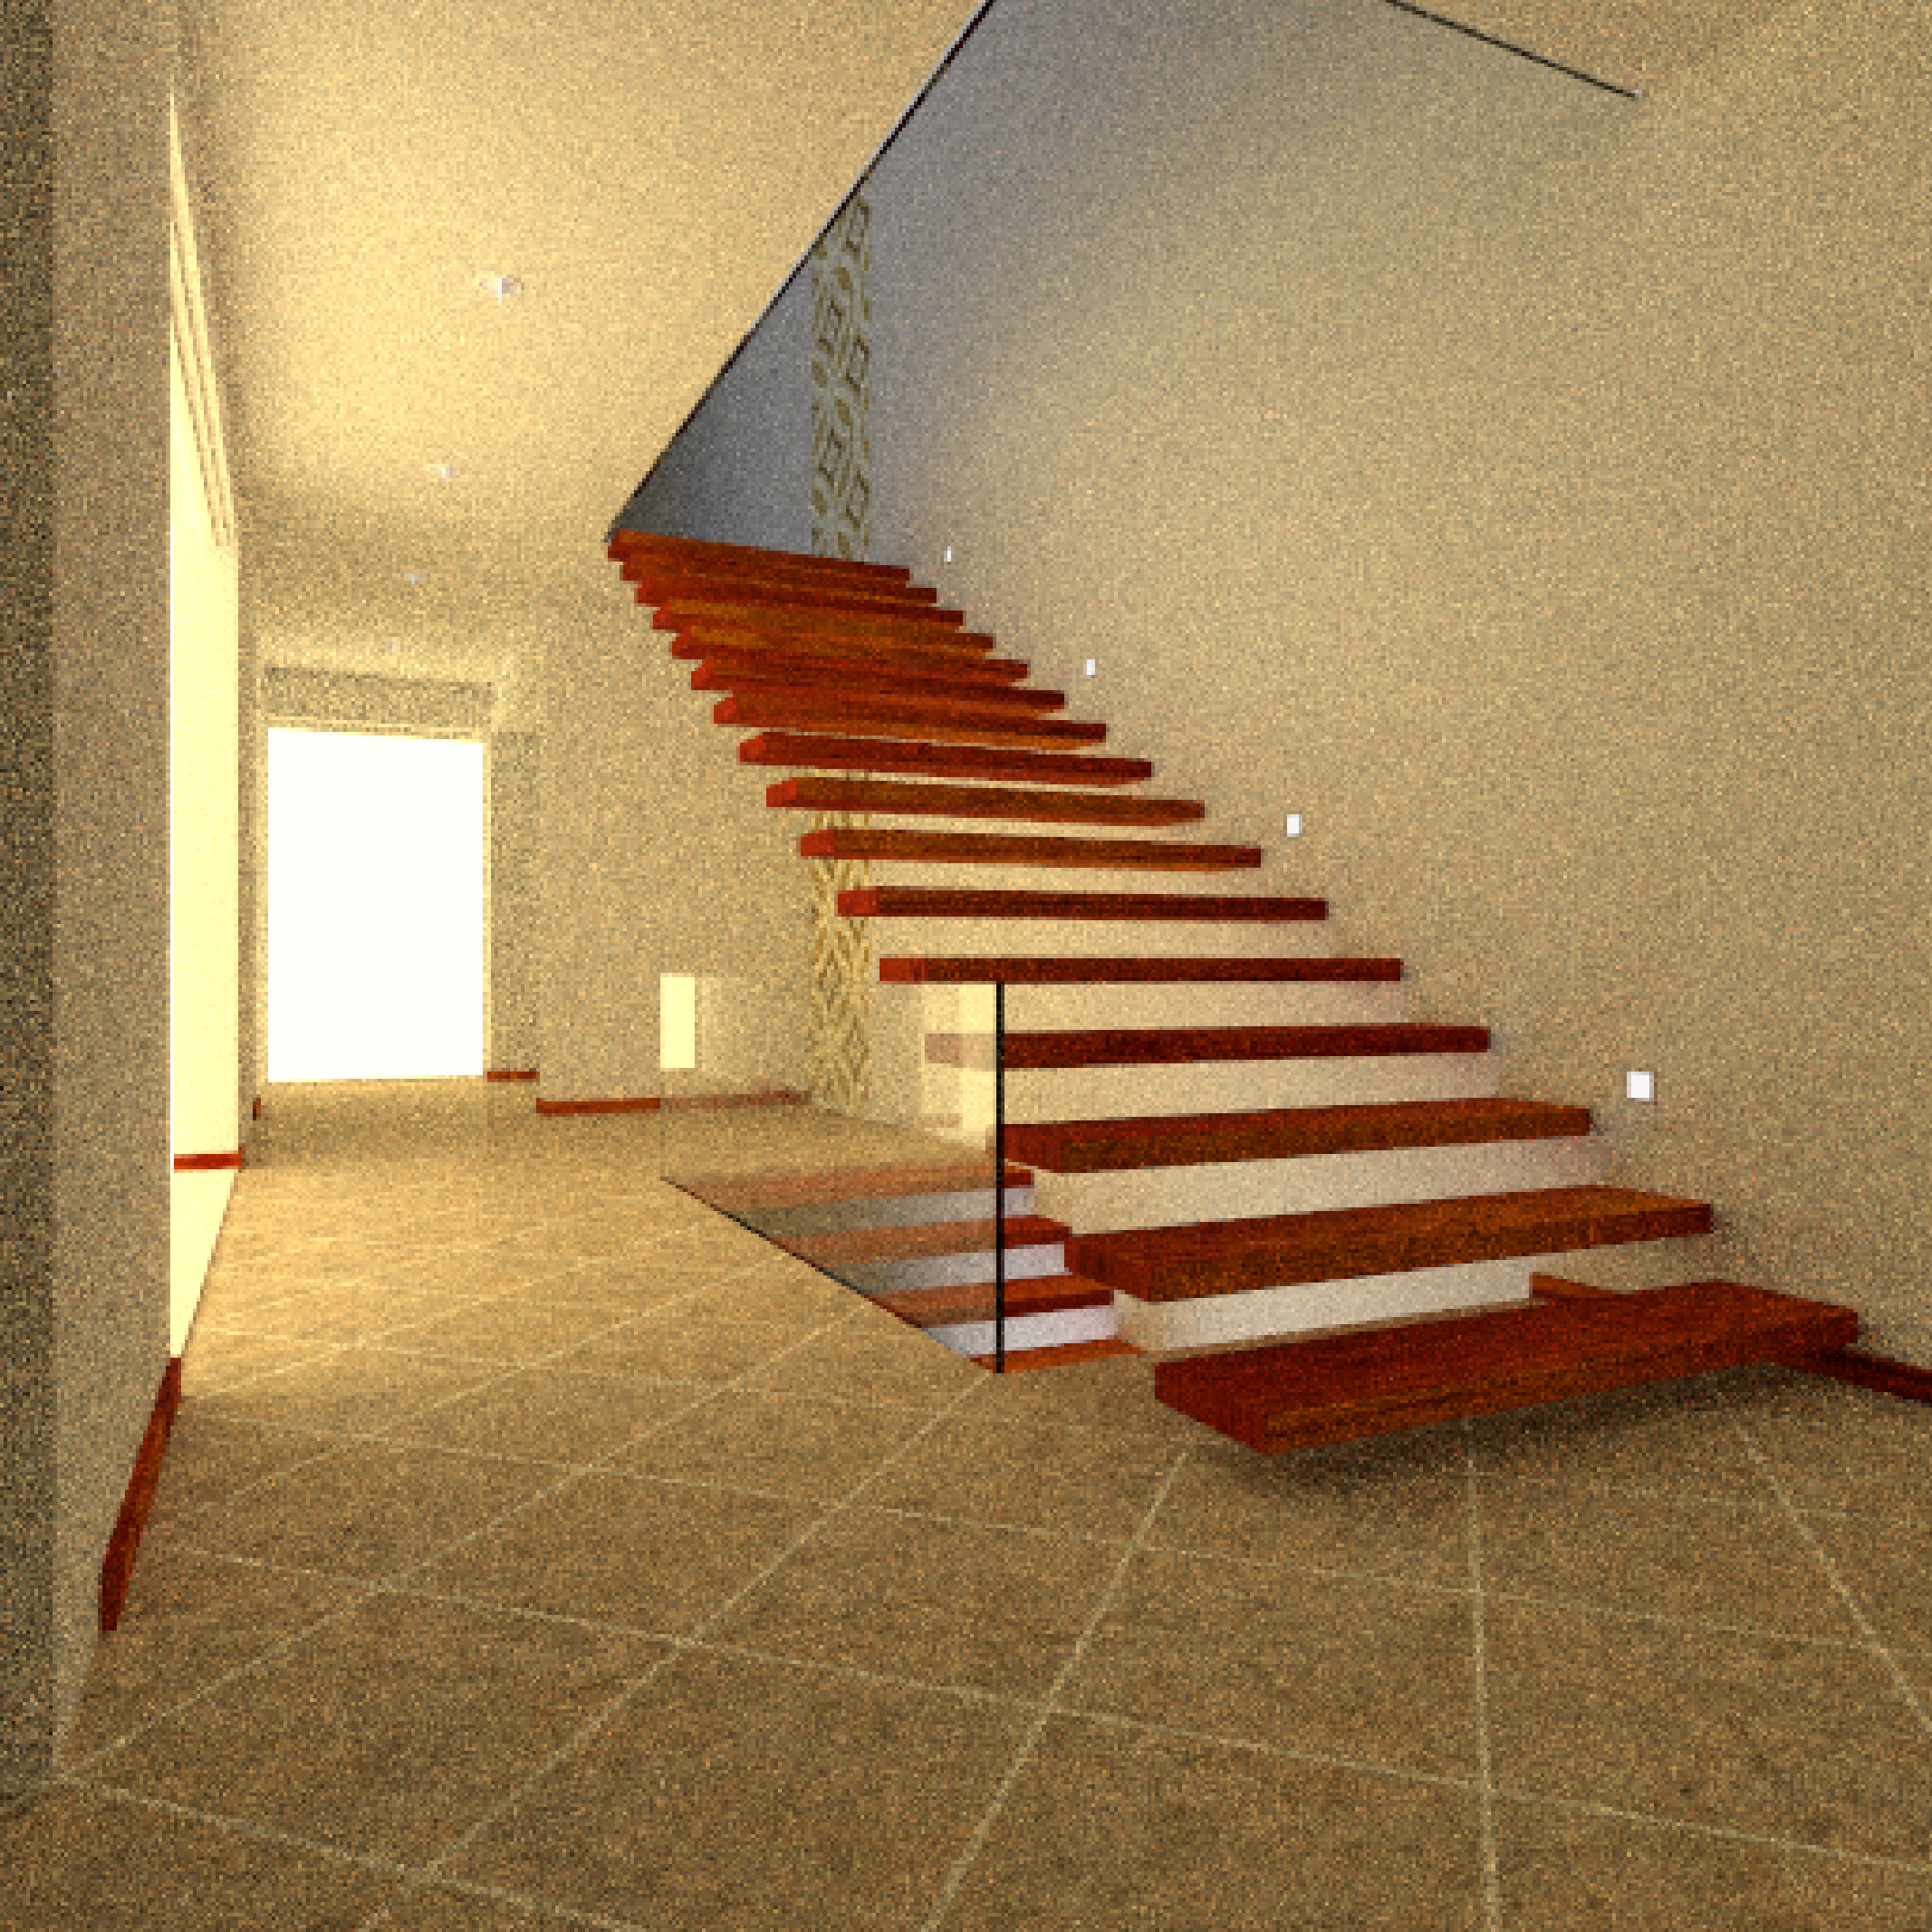
\includegraphics[height=8cm]{chapters/chapter_thetool/hall}
	\caption{\textit{Modern Hall} scene \cite{bitterliscenes} rendered by Yocto/GL \cite{pellacini2019yocto}. It is a 512x512, 512spp image; maximum bounces per path are set to 10.}
	\label{hall_render}
\end{figure}
As said just above, the paths in this case bounce at most 10 times: most paths are terminated way before either when they bounce out of the scene or --- in some path tracers --- they hit a light. This leads to the need of an additional buffer storing the amount of bounces each path has. Put with computer graphics terminology we might say the points positions buffer represents the \textit{geometry} of the paths while this “path lengths” buffer is the \textit{topology}. 
This new buffer needs to contain integers and, considering that the standard C++ \texttt{int} built-in type on x86\_64 machines is 4 bytes long, we would have that the size of the buffer in the context of figure \ref{hall_render} would approximately be:
\begin{equation}
	\label{rough_lenghts_size_estimation}
	(512 \times 512) pixels \times 512 spp \times 4 bytes \approx 500MB
\end{equation}
Now this is not an unmanageable amount of data, but since the tool has to be usable on consumer grade machines, reducing those number has been one of the main priorities during the early stages of development. The most effective change that has been made is to simply use smaller primitive data types. 
Single precision floats had been almost immediately replaced with half-precision floating point numbers, effectively halving the size of the world positions buffers. Using the same assumptions made for equation \ref{rough_bounce_size_estimation}, we would have 7.5GB instead of 15GB.
Halving precision, beside a memory footprint reduction, comes with a reduction of actual precision and potential noticeable rounding errors; but since these numbers will mostly be directly used for visualization purposes with very little preprocessing, precision errors should not negatively impact the user experience.
Considering now the paths lengths buffer, in most reasonable cases, 1 byte per path would suffice: 255 bounces are more than enough for most cases. Examining equation \ref{rough_lenghts_size_estimation}, after the reduction from 4 bytes to 1 that buffer occupies approximately 128MB. Similar reasoning has been applied to all other buffers: every floating point number is half precision and every integer is made as small as reasonable.

To complete the spatial representation of the paths, an origin point, which is semantically not a bounce, was needed. For the sake of simplicity, an additional fake bounce lying on the render camera eye was added to each path. Due to its wasteful nature --- it adds 6 bytes per path which would accumulate to $512\times 512\times 512\times 6\approx 750MB$ in the case of figure \ref{hall_render} ---, this solution was hastily set aside; in the final version of the tool, the origin point of the paths is not stored in the dataset all together. The camera eye point that comes with the scene description --- see subsection \ref{scene_format} --- is implicitly considered the origin of all paths.

To fuel some components of the visualization client that have been developed over time, two other buffers are built by \texttt{gatherer}. One contains the camera samples and the other the radiance carried by each path. A camera sample is the correct position of a path on the virtual image sensor. The radiance of each path is just stored as a triplet of floats indicating the radiance carried by a path for the red, green and blue color components.

Focusing on implementation details it is clear that four binary data buffers have to be stored on disk. They could all be cramped into a single file but to make the loading code simpler, it has been decided to store each buffer in its own separate file.
This means that a full dataset has to be contained into a folder rather than a file. The folder, usually, but not necessarily, called \texttt{renderdata} contains two subfolders, \texttt{bounces} and \texttt{paths}.
This was made to logically separate buffers that contains data proper to entire paths --- like the lengths and the radiances --- to the ones relative to bounces --- the bounces positions. It may seem a little overzealous but it was made to support an easy and organized implementation of new buffers.

At the end of the day, there are 4 binary files and each contain:
\begin{description}
	\item[\texttt{bounces/positions.bin}] The world positions of all bounces of each path, stored as triplets of \texttt{half}.
	\item[\texttt{paths/lengths.bin}] The number of bounces of each path --- almost always called \textit{path length} in the code ---, each stored as a single \texttt{uint8\_t}.
	\item[\texttt{paths/radiance.bin}] The radiance carried by each path, stored as triplets of \texttt{half}.
	\item[\texttt{paths/camerasamples.bin}] The sample position on the film plane of each path. Each sample is stored in a \texttt{CameraSample} data structure\footnote{See listing \ref{gatherer_datastructures} for the actual C++ definition.}, which contains:
	\begin{itemize}
		\item A couple of \texttt{uint16\_t} indicating which pixel of the render image the sample belongs to.
		\item A couple of \texttt{half} $\in [0, 1]$ representing the position of the sample relative to the pixel, where $(0,0)$ is the upper left corner of the pixel and $(1,1)$ is the lower right one.
	\end{itemize} 
\end{description}

%TODO: maybe add an explanation on how is easy to understand which data is relative to which path?

\subsection{\texttt{Gatherer} class}
All data gathering is managed by a header-only library that exposes one single class called \texttt{Gatherer}. To correctly gather data from a path tracer the user must initialize an instance of \texttt{Gatherer} at any point before the main loop and then call its methods where appropriate while tracing paths. Signatures of the constructor and the methods of \texttt{Gatherer} is presented in Listing \ref{gatherer_signatures}.
The constructor needs a folder path where the data will be stored and the number of threads --- \texttt{nthreads} --- the path tracer will run on. The \texttt{addbounce} method has to be called every time a path bounces and the position of the bounce is final. It has that position in world coordinates as an argument  alongside a \textit{thread id}, an integer that goes from zero to \texttt{nthreads} and unequivocally identifies a thread.
When all the computations on a path are done and the radiance carried by it is known, the user has to call the \texttt{finalizepath} method passing the thread id, the radiance and a \texttt{CameraSample} struct --- see Listing \ref{gatherer_datastructures} for its layout.

As hinted by the \texttt{nthreads} and \texttt{tid} arguments of \texttt{Gatherer} methods, the class has been designed to be able to gather data from path tracers that evaluate paths on multiple threads parallelly. This extra effort has been made to not force users to use only single-threaded path tracers. It has to be though noted that the \texttt{Gatherer} class assumes each path is entirely resolved on just one thread: splitting the computations of a single path on multiple threads is not currently supported.

Datasets gathered from the rendering of high quality scenes can get big fast. To avoid any memory saturation problems and to leave as many resources as possible to the path tracing computations, \texttt{Gatherer} allocates a fixed amount of memory per thread and will use only that; it will store data on disk when any of these memory chunks are about to fill completely. In order to write to disk without introducing any software barrier in the multi thread code, each thread writes on a set of files that are written only it. The destructor of \texttt{Gatherer} takes care of stitching all these file sets into one, being extra careful to keep the indices consistent. This is sadly a fully disk-bound operation and it may take a while, especially on rather big dataset.


\begin{Listing}
	\begin{lstlisting}
class Gatherer
{
public:
	Gatherer
	(
		unsigned nthreads, 
		const std::filesystem::path& folder
	);

	void addbounce
	(
		unsigned tid, 
		Vec3h pos
	);

	void finalizepath
	(
		unsigned tid, 
		Vec3h radiance, 
		CameraSample sample
	);
}
	\end{lstlisting}
	\caption{Simplified \texttt{Gatherer} class definition with everything a user needs to gather data successfully.}
	\label{gatherer_signatures}
\end{Listing}

\begin{Listing}
	\begin{lstlisting}
using Vec3h = std::array<half, 3>;

class CameraSample
{
public:
	uint16_t i, j;
	half u, v;
};
	\end{lstlisting}
	\caption{Data structures used inside the \texttt{Gatherer} class. The \texttt{half} type contains a 16bit precision floating point number complying to the IEEE 754 standard.}
	\label{gatherer_datastructures}
\end{Listing}

%\begin{lstlisting}[caption={}, label=scene_json]
%\end{lstlisting}

\section{Visualization client}

\subsection{Path filters}
\label{path_filters}

\begin{figure}
	\centering
	\begin{subfigure}[t]{0.49\linewidth}
		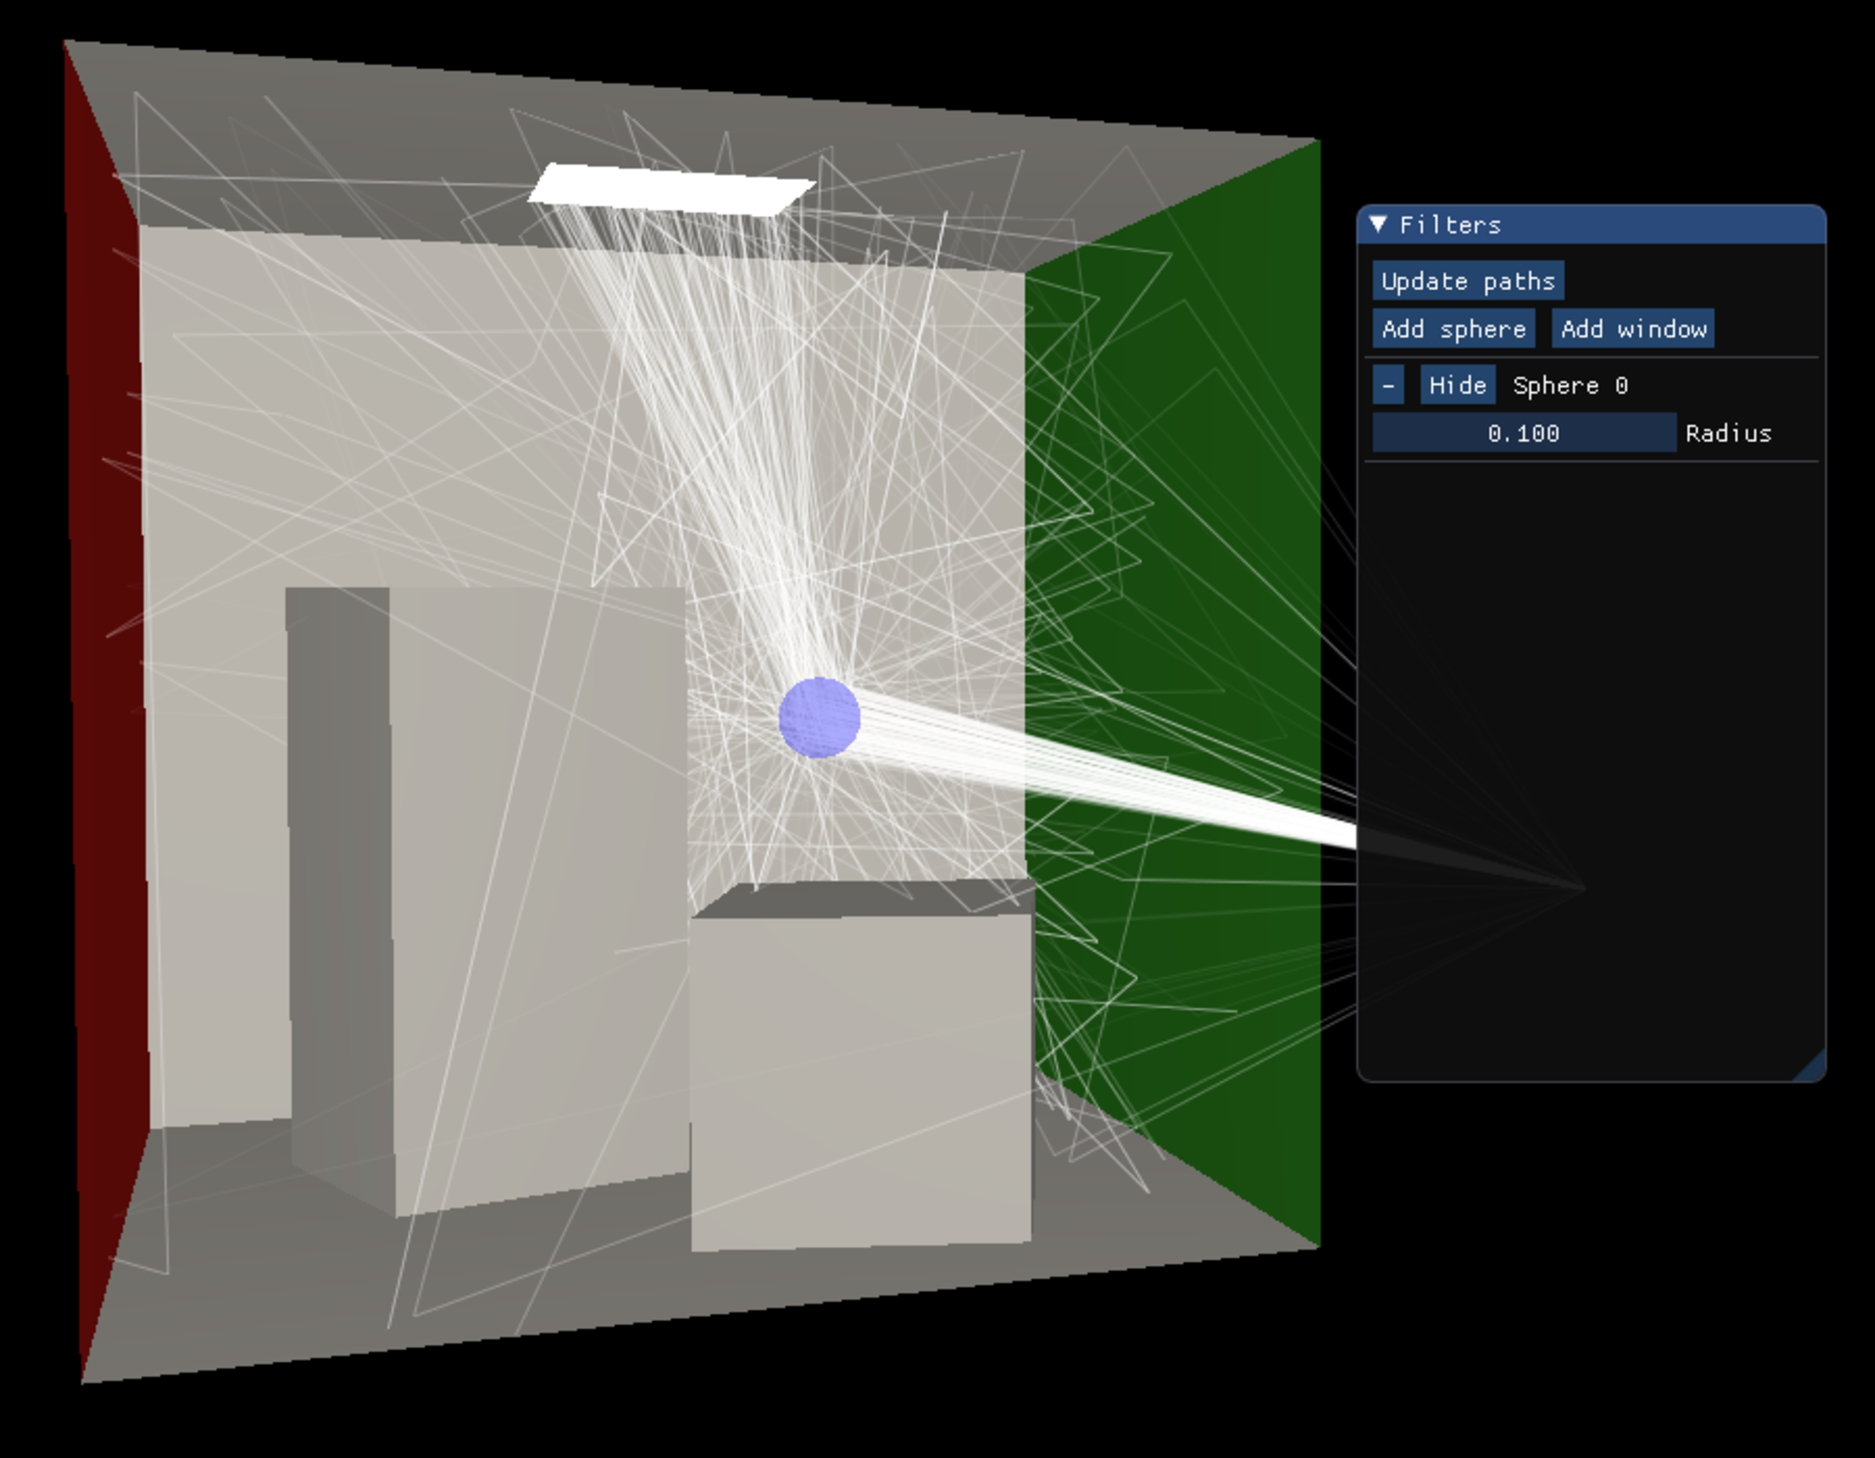
\includegraphics[width=\textwidth]{chapters/chapter_thetool/filterscombination1.pdf}
		\caption{In the beginning, one sphere is placed on the back wall.}
	\end{subfigure}
	\begin{subfigure}[t]{0.49\linewidth}
		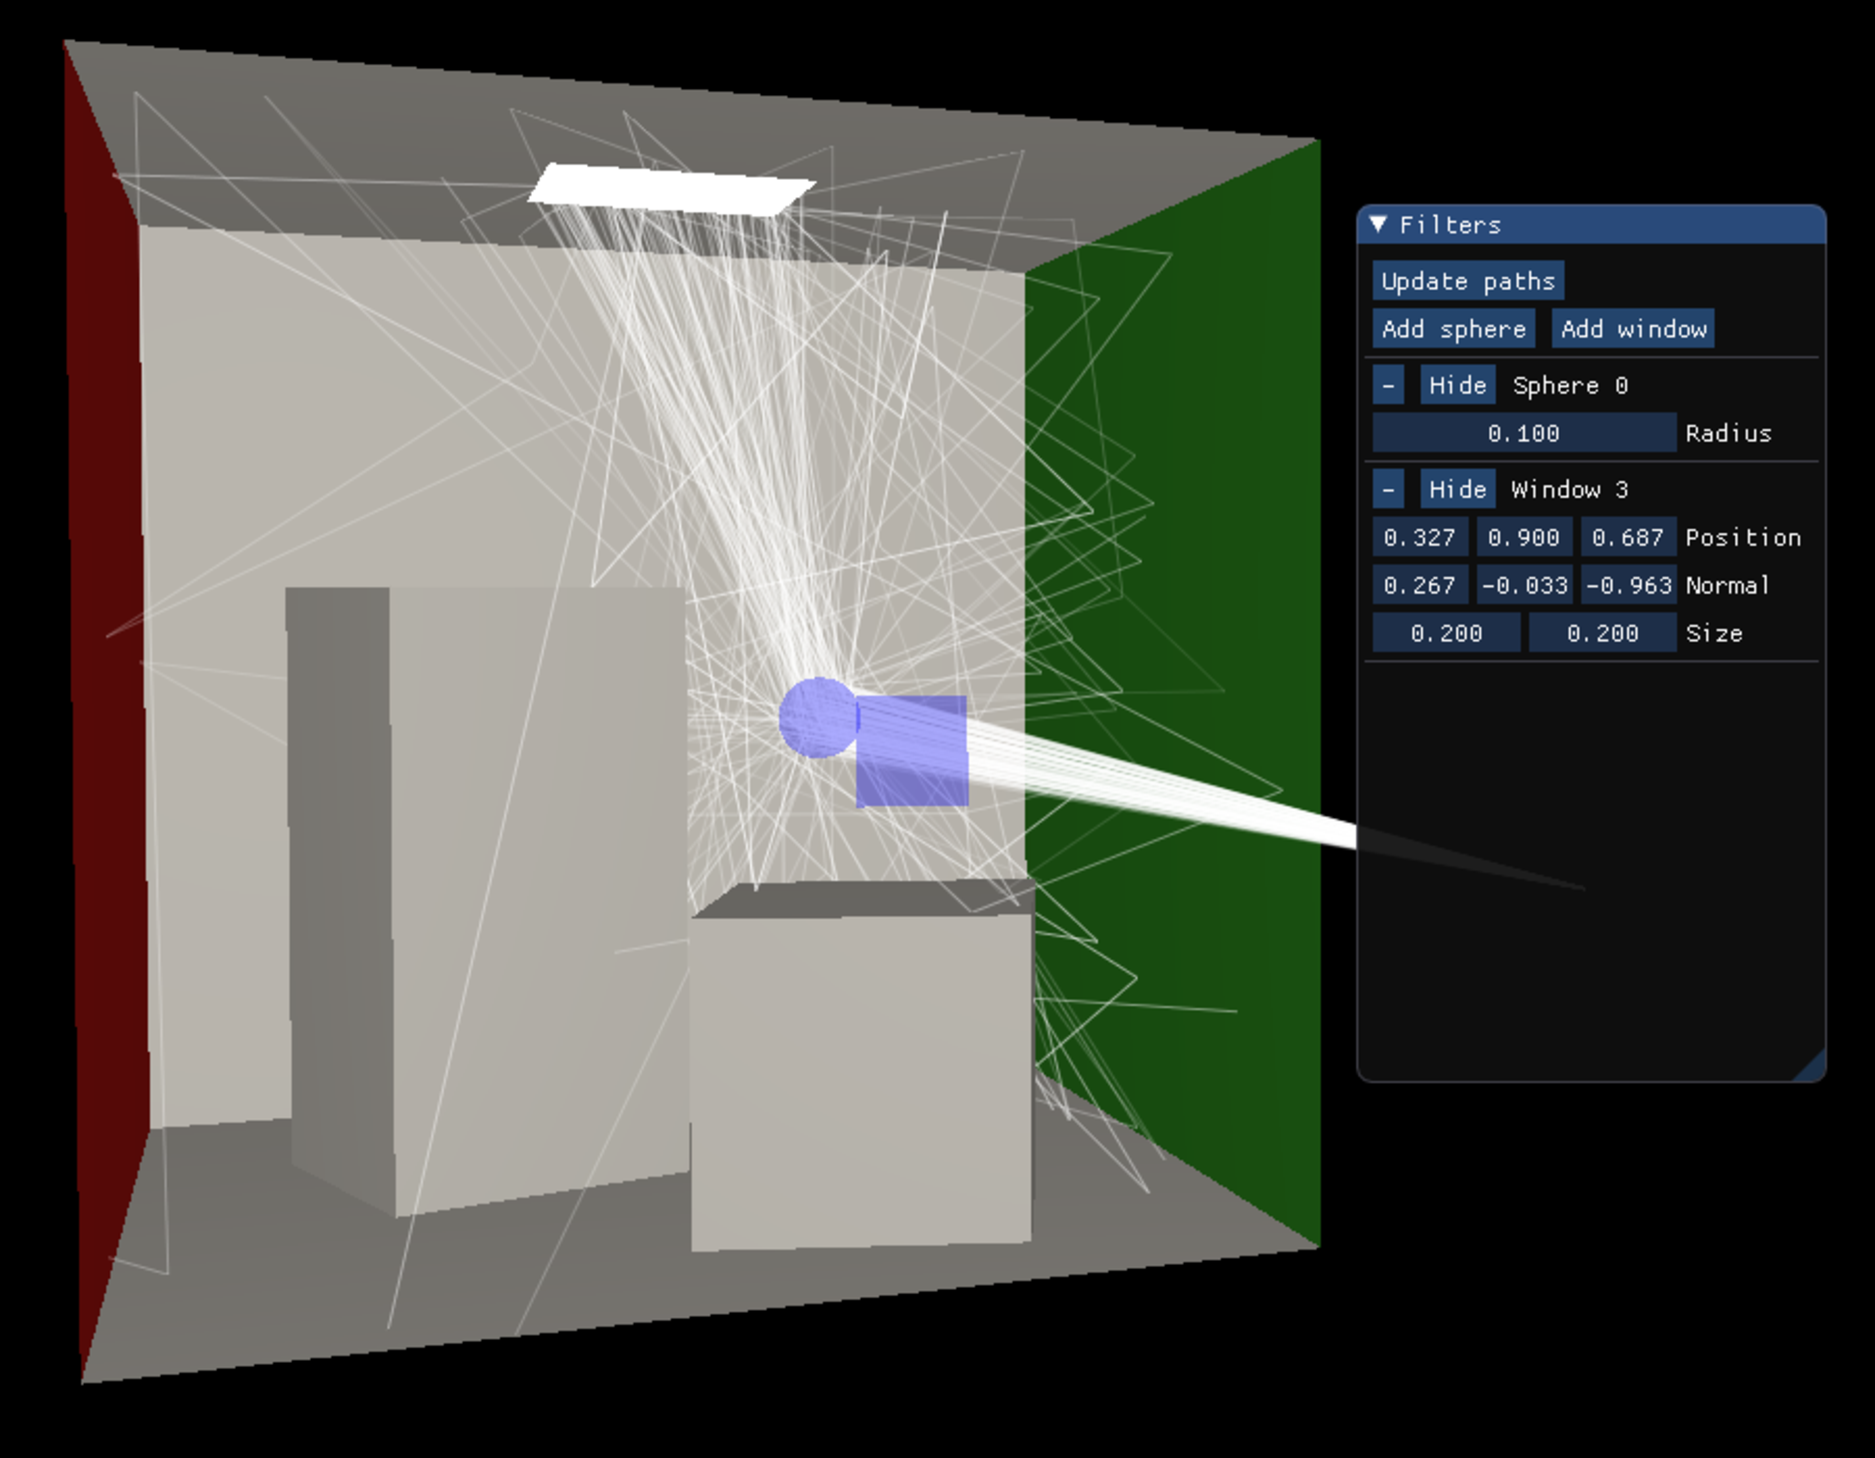
\includegraphics[width=\textwidth]{chapters/chapter_thetool/filterscombination2.pdf}
		\caption{Then a window is placed to select only the paths that go from the camera to the sphere on the back wall.}
	\end{subfigure}
	\begin{subfigure}[t]{0.49\linewidth}
		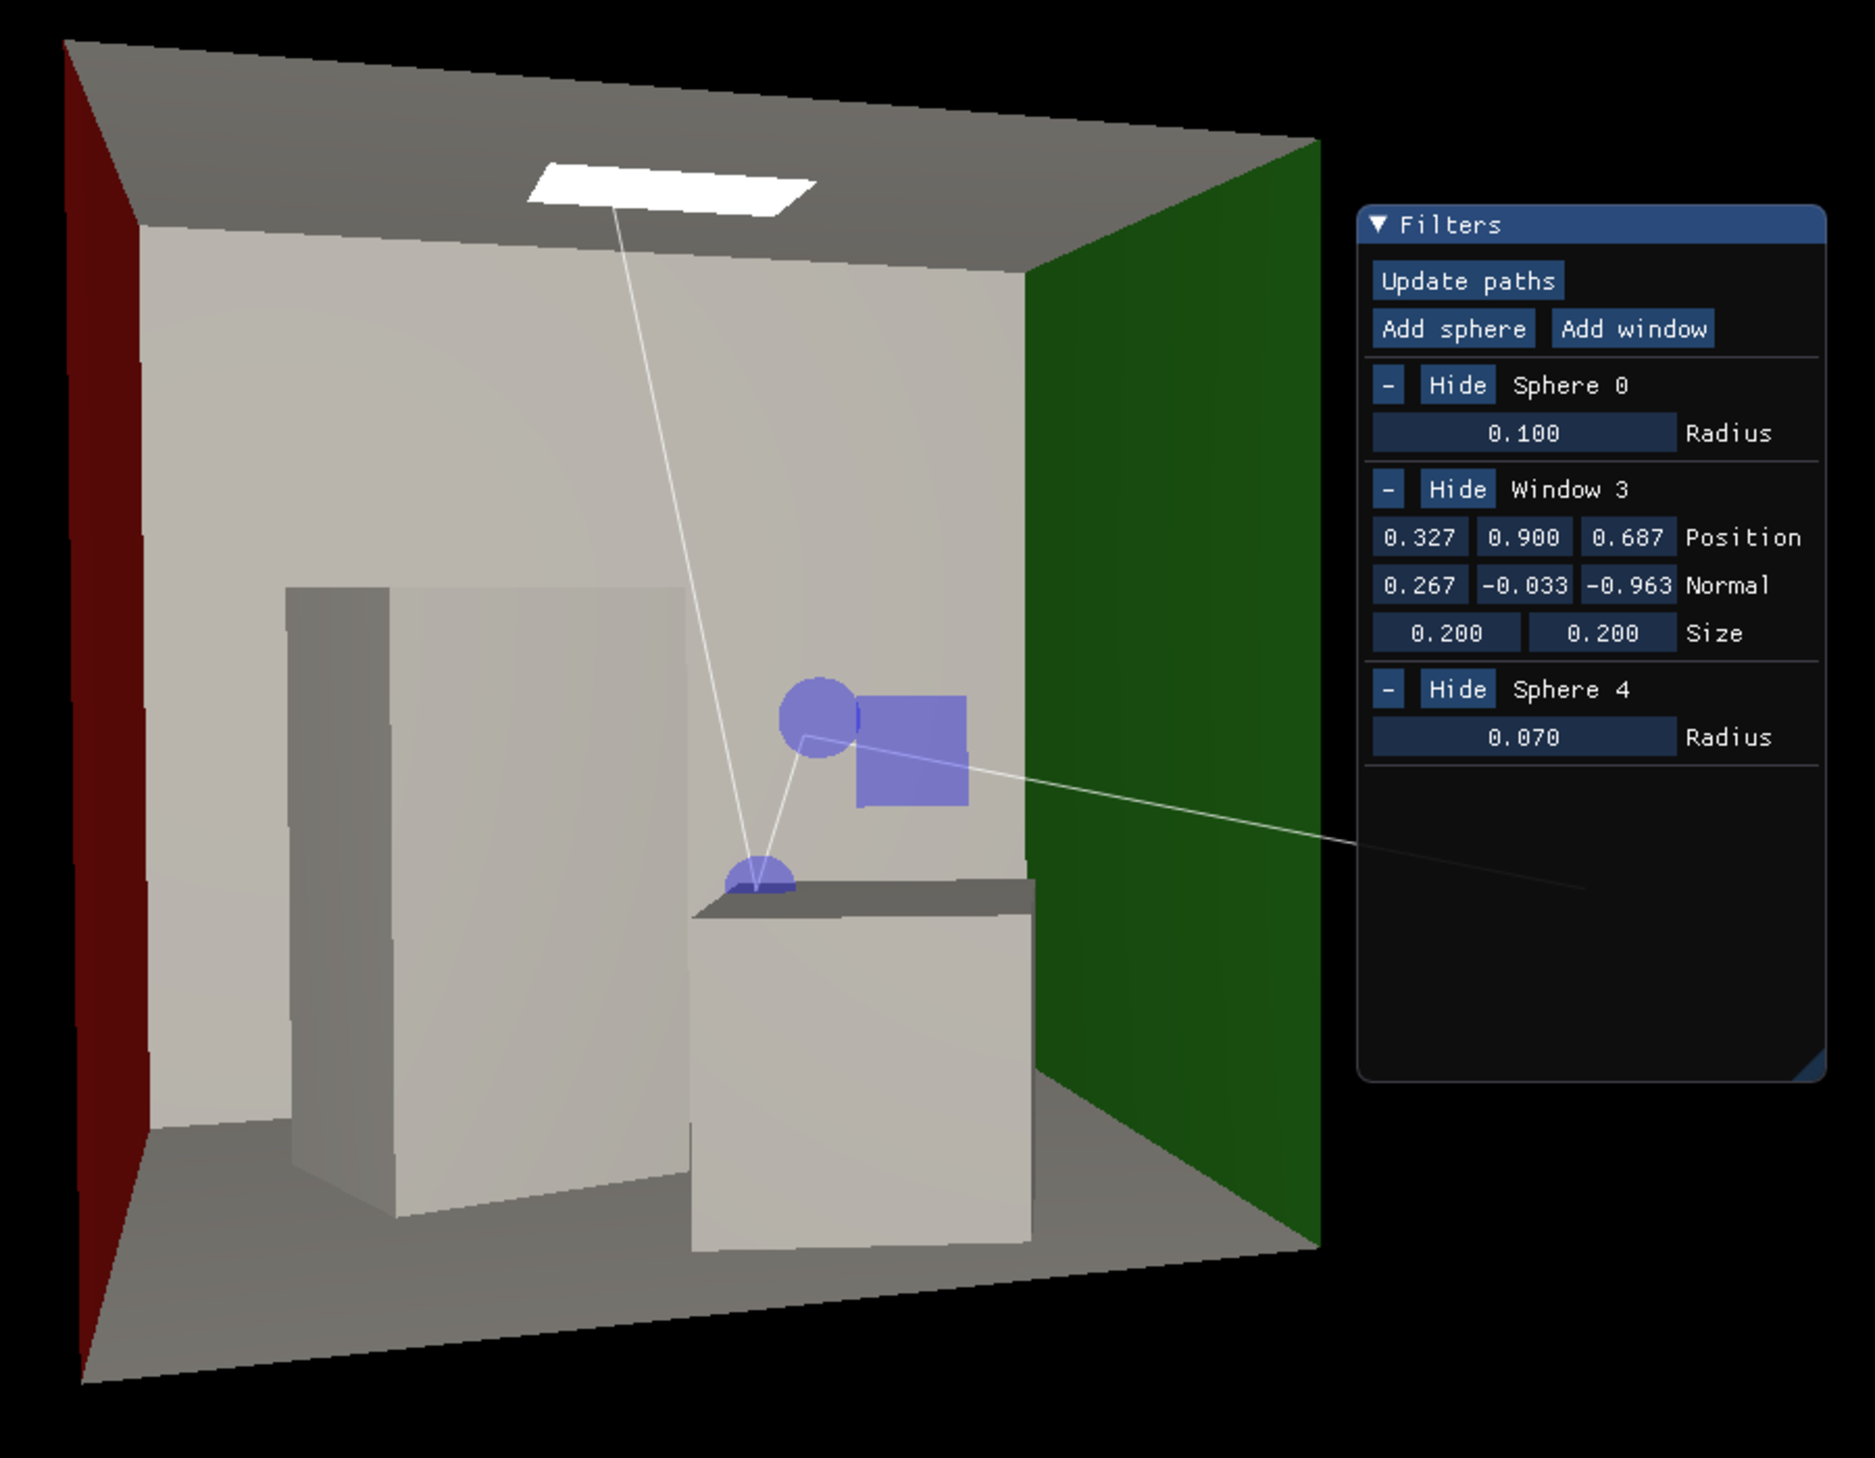
\includegraphics[width=\textwidth]{chapters/chapter_thetool/filterscombination3.pdf}
		\caption{Finally, a second sphere is placed on top of the short box to select only a single path.}
	\end{subfigure}

	\caption{Example of using more path filters together in a small dataset generated on the Cornell Box scene of $64 \times 64$ pixels and 32 spp.}
	\label{filterstack}
\end{figure}

As said already, visualizing all paths at once is both useless and impossible in most cases. User can filter paths so they can focus only on the scene portions they are interested in. Two filters types are provided: the \textit{sphere filter} and the \textit{window filter}. The former is a sphere that has to be placed on a scene surface and selects the paths bouncing inside its radius, the latter is a rectangular window that selects the paths passing through it.

As shown in figure \ref{filterstack}, combination of filters of both kinds can be used together. Considering all paths as a mathematical set of distinct paths $\mathcal{S}$, a filter $F$ creates a subset $F(\mathcal{S}) \subseteq \mathcal{S}$, and combining the filters $F_1, F_2, ..., F_n$ gives the intersection of their relative subsets:
\begin{equation}
	\label{filters_union}
	F_1(\mathcal{S}) \cap F_2(\mathcal{S}) \cap ... \cap F_n(\mathcal{S}) \subseteq \mathcal{S}
\end{equation}
Due to this strong affinity to mathematical sets, the initial code handling the filters' combination was mostly based on the \texttt{std::set<T>} data structure of C++ standard library. It was put apart when it turned out to be significantly slower than just storing everything into \texttt{std::vector<T>} structures and performing set intersections with the \texttt{std::set\_intersection} function from the \texttt{<algorithm>} STL library. To further speed the filtering up, the filters are computed in order so they all need to just test the paths selected by the previous filter; in the implementation, equation \ref{filters_union} is practically evaluated as if it was:
\begin{equation}
	F_n( ... F_2(F_1(\mathcal{S}))) \subseteq \mathcal{S}
\end{equation}
The tool uses a \texttt{std::vector<unsigned>} called \texttt{selectedpaths} to keep the indexes of the currently selected paths. Each filtering step is practically run over the \texttt{selectedpaths} output by the last stage. Before any filter, \texttt{selectedpaths} is filled with all path indexes. Forcing this into mathematical notation gives that the $i$th filter step out of $m$ filters is:
\begin{equation}
	\texttt{selectedpaths}_i = F_i(\texttt{selectedpaths}_{i-1}),\ i\in[1, m]
\end{equation}
where $\texttt{selectedpaths}_i$ is the \texttt{selectedpaths} vector after filtering through the $i$th filter and $\texttt{selectedpaths}_0 = \mathcal{S}$.

Users can add, modify and delete filters from the \textbf{“Filters”} floating panel. On the top of it there are three push buttons:
\begin{description}
	\item[“Update paths”] Since path filtering is an operation that takes a noticeable time to complete, the user must explicitly express the will to apply the current filter set to the paths.
	\item[“Add sphere”] After the user clicks this, they have to click on a surface of the scene. A filter sphere will appear on the clicked surface.
	\item[“Add window”] Same as the previous button but it adds a window filter on the clicked scene surface instead.
\end{description}
Filters currently present in the scene will appear right below these buttons. Each filter has an entry and all of these will have a delete button --- marked with a minus \textbf{“-”} sign ---, a \textbf{“Hide”}/\textbf{“Show”} button to toggle the filter visibility in the viewport, and a label with the filter name. Then, according to their filter type, there will be sliders controlling miscellaneous attributes.

\subsubsection{Sphere filter}
This was the first filter added. It has a spherical shape and simply selects all the paths having at least one bounce inside its volume. Users can place a sphere filter on clicking on any scene surface on the viewport after having clicked the \textbf{“Add Sphere”} button at the top of the \textbf{“Filters”} panel. Once a sphere filter has been added, its radius can be controlled by the slider in its slot on the panel. The default radius is one tenth of the scene's largest dimension. One possible future improvement would be giving the possibility to translate the sphere after it has been initially created; might this be achieved through 3d gizmos or just by dragging, every step in that direction should help the usability.

The actual path filtering is plainly done by computing the squared distance between each bounce of each path and the sphere center. For each bounce with a computed distance less than the sphere radius, its entire path gets flagged as selected. This allows for a path-wise early termination: if a path has been flagged, it is useless to check the remaining bounces of the same path. Early termination or not, this computation is rather heavy since a render dataset rarely goes under the one hundred million bounces mark. To mitigate the otherwise lengthy waiting times, the computation is done on multiple threads; The set of paths that has to be filtered is divided in $n$ subsets $S_{1...n}$ of roughly the same cardinality, where $n$ is the number of maximum thread concurrency available on the machine. Each subset is coupled with a \texttt{std::vector<unsigned>} that has to hold the indexes of the paths of the subset that satisfy the filter; to avoid memory allocations, these vectors reserve $|S_{1...n}|$ slots each before any computation. Then, $n$ threads start to apply the filter to their assigned subset. Once all of them are done, the content of the vectors --- which are the indexes of the selected paths by each thread --- are moved into \texttt{selectedpaths}, the STL vector keeping the index of all selected paths.

On the viewport the spheres are rendered without passing any vertex buffer to the GPU: first, using hard-coded coordinates and the GLSL \texttt{gl\_VertexID} built-in variable, a cube of side 2 centered on the origin is generated on the vertex shader; then through tessellation new vertices are generated --- every patch level has been set to 3 --- and then displaced on the surface of a unit sphere. Finally scaled and transformed at the end of the tessellation evaluation shader, the resulting triangles are ready to rasterize.

\subsubsection{Window filter}
The window filter is a rectangle embedded in 3d space that selects all the paths passing through it. After clicking on \textbf{“Add Window”} button, user can spawn a window filter by clicking on a surface; a window facing the camera with its central point lying on the clicked surface will be created. The filter can then be translated, rotated and scaled through the many sliders available in the filter slot on the \textbf{“Filters”} panel. The current interface is rather difficult to use and many things can be done to improve it, such as 3d gizmos, as already suggested for the sphere filter.

The filtering is performed by iterating over the paths and for each test if any of its rays intersect the window. Even this filter supports the same kind of path-wise early termination presented for the sphere filter. To perform the ray-window intersection test, a slightly modified version of the M\"oller-Trumbore algorithm \cite{moller1997fast} has been employed: each ray, instead of being tested  against the two co-planar triangles that make up the window, is actually tested against a single large triangle encompassing the window, like shown in figure \ref{encompassing_triangle}; then, rays intersecting the triangle on points with any of the barycentric coordinates relative to the hypotenuse's vertices greater than $0.5$ are discarded.
\begin{figure}
	\centering
	\begin{tikzpicture}
		\draw[pattern=crosshatch dots] (0,0) rectangle (1.5,1);
		\draw (0,0) -- (0,-1) -- (3,1) -- (1.5,1);
	\end{tikzpicture}

	\caption{The triangle encompassing a window filter (dotted). It is just a right triangle of which right angle lies on a window vertex and of which catheti are as long as twice the window sides.}
	\label{encompassing_triangle}
\end{figure}	


\subsection{Viewport}
The 3-dimensional viewport is the central component of the visualization tool. It takes care of interactively rendering three entities: the scene geometry, the paths' rays and the filters shapes. Each presented their own challenges that culminated in the implementation of their cross interactions. Having these many elements to show brought the necessity of employing multi-pass rendering, compositing techniques throughout the render pipeline and consequent multiple frame buffers. To save resources and keep the UI snappy even when the viewport requires most GPU resources, the viewport renders only when a change of any visualization parameter or scene/dataset properties happens. For this purpose, a boolean variable called \texttt{mustrenderviewport} is used and has to be set true to require a viewport redraw. The render pipeline and the interface controls provided to the user to tweak its stages will now be explained analyzing the steps made to render figure \ref{viewport_render}.

\begin{figure}
	\centering
	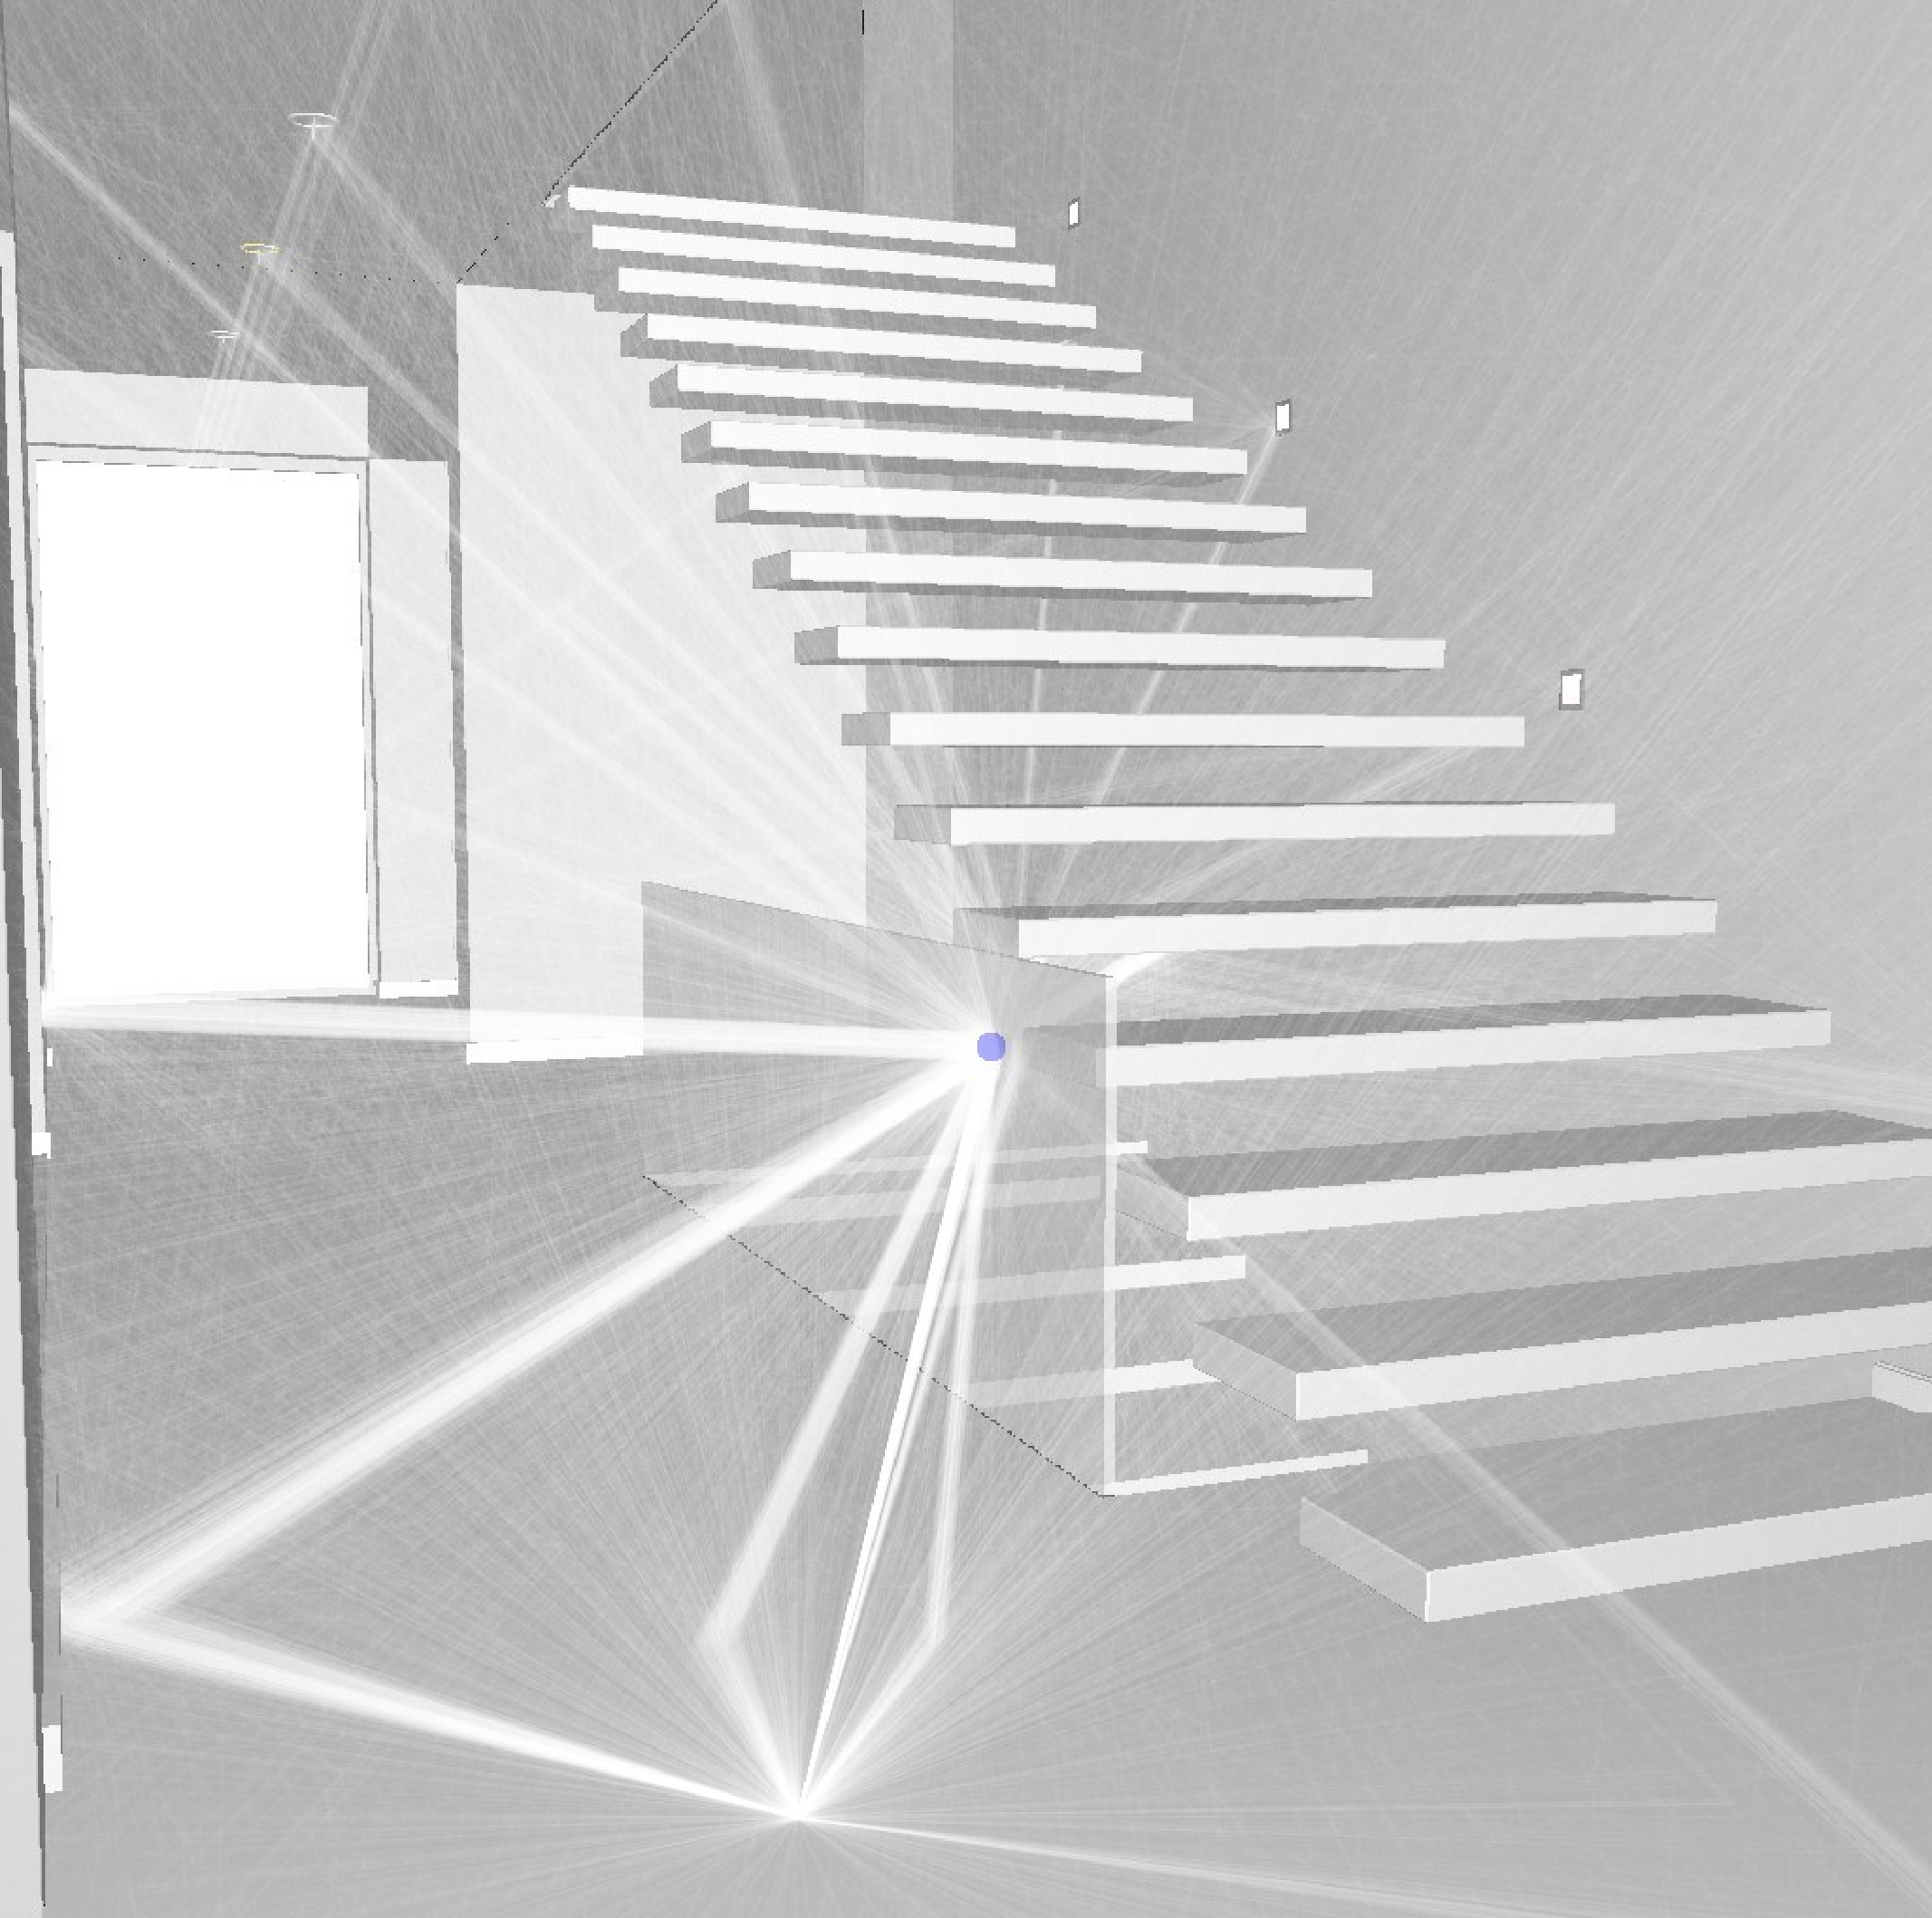
\includegraphics[height=8cm]{chapters/chapter_thetool/viewport_render.pdf}
	\caption{An example of a final frame rendered by the viewport.}
	\label{viewport_render}
\end{figure}

The scene is rendered in two passes, one for the opaque geometries and the other for translucent ones. The opaque geometries pass is done first and outputs a \textit{beauty} texture, the \textit{world positions} texture, the \textit{geometry ID} texture, and a \textit{depth} texture. The beauty texture (fig. \ref{beauty_scenepass1}) is a color render of the scene lighted by a point light placed on the camera. Every surface is flat shaded with a plain Lambertian model \cite{lambert1760photometria}. As detailed in section \ref{scene_format}, the scene format does not store the vertex normals, instead the surface normals are computed on the fragment shader using the \texttt{dFdx} and \texttt{dFdy} GLSL functions on the world position of the fragments. As their names suggest, the world position, geometry ID and depth textures (fig. \ref{worldpos_scenepass1}, \ref{worldposa_scenepass1} and \ref{depth_scenepass1}) respectively store the world position, geometry ID and the depth --- which is distance from the camera $\in[0,1]$, where 0 is on the near clipping plane and 1 is on the far clipping plane --- of each fragment. Having depth data might seem redundant when the world positions are available, but to take advantage of the built-in depth testing functionalities of OpenGL it has been preferred to keep both textures. The world positions and geometry IDs are used to get information on the points clicked by the user; these are then used for example, when placing filters or selecting scene objects to hide.

\begin{figure}
	\centering
	\begin{subfigure}[t]{0.24\linewidth}
		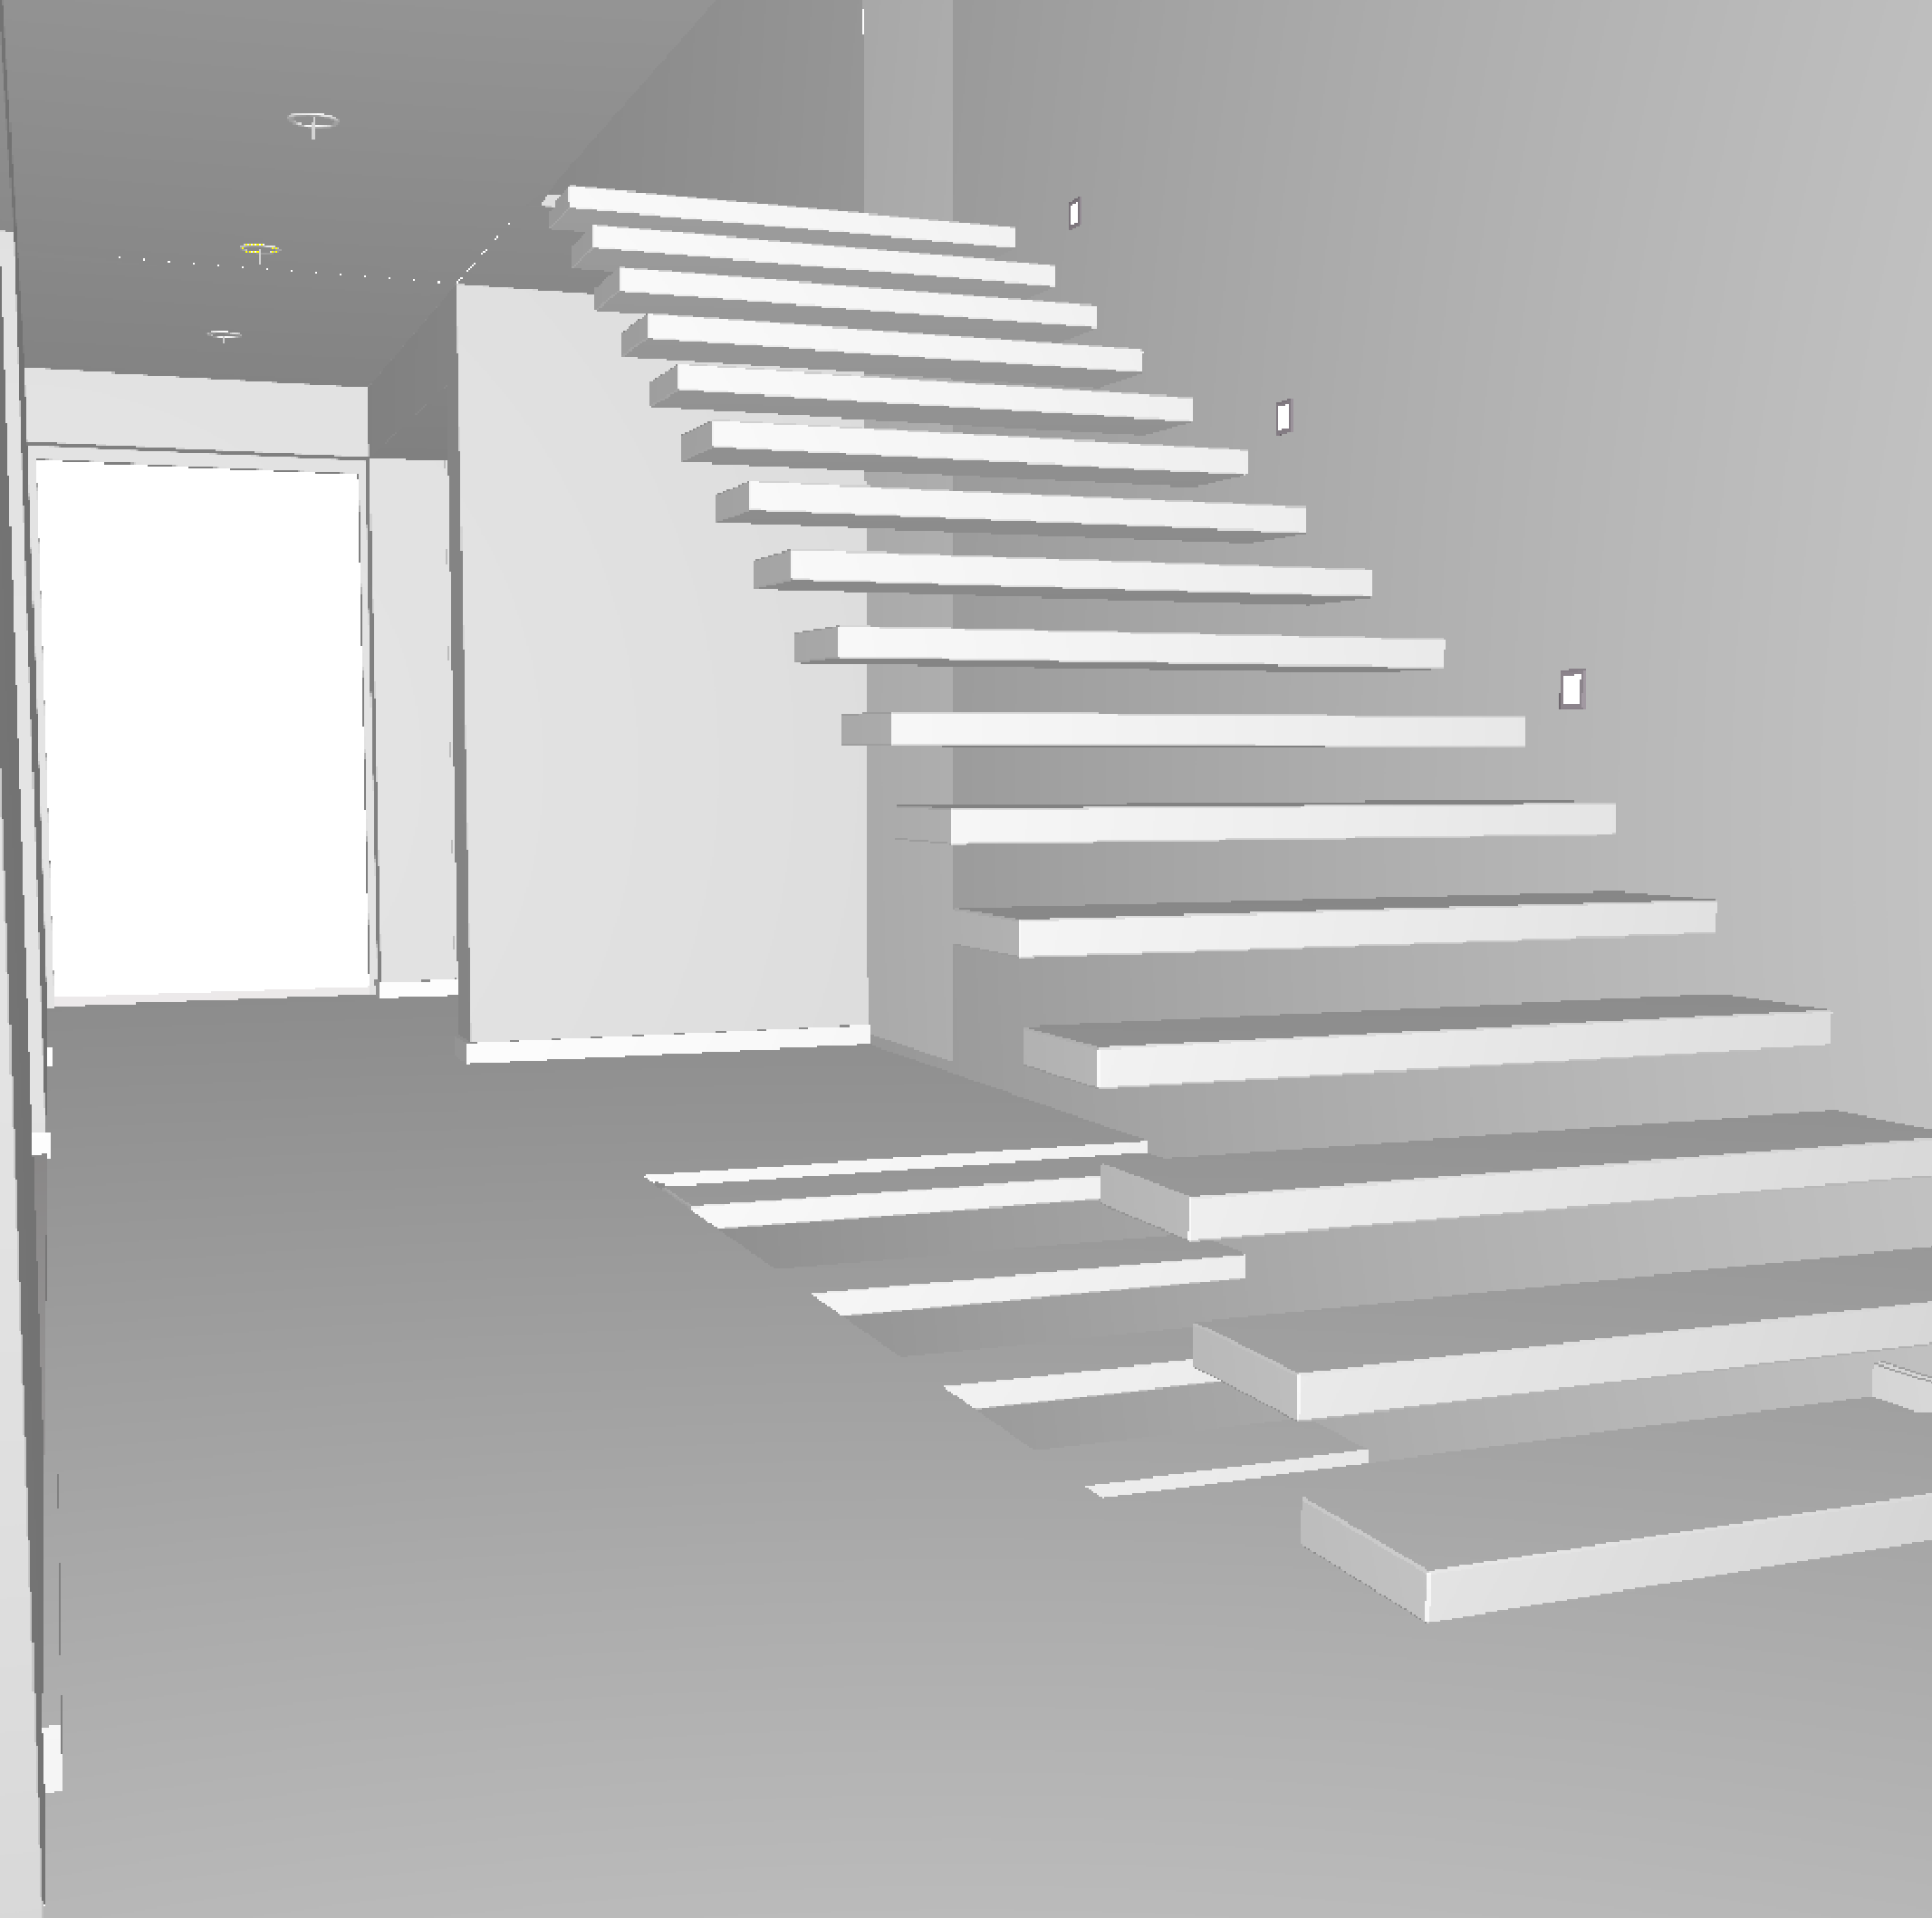
\includegraphics[width=\textwidth]{chapters/chapter_thetool/beauty_scenepass1}
		\caption{Beauty}
		\label{beauty_scenepass1}
	\end{subfigure}
	\begin{subfigure}[t]{0.24\linewidth}
		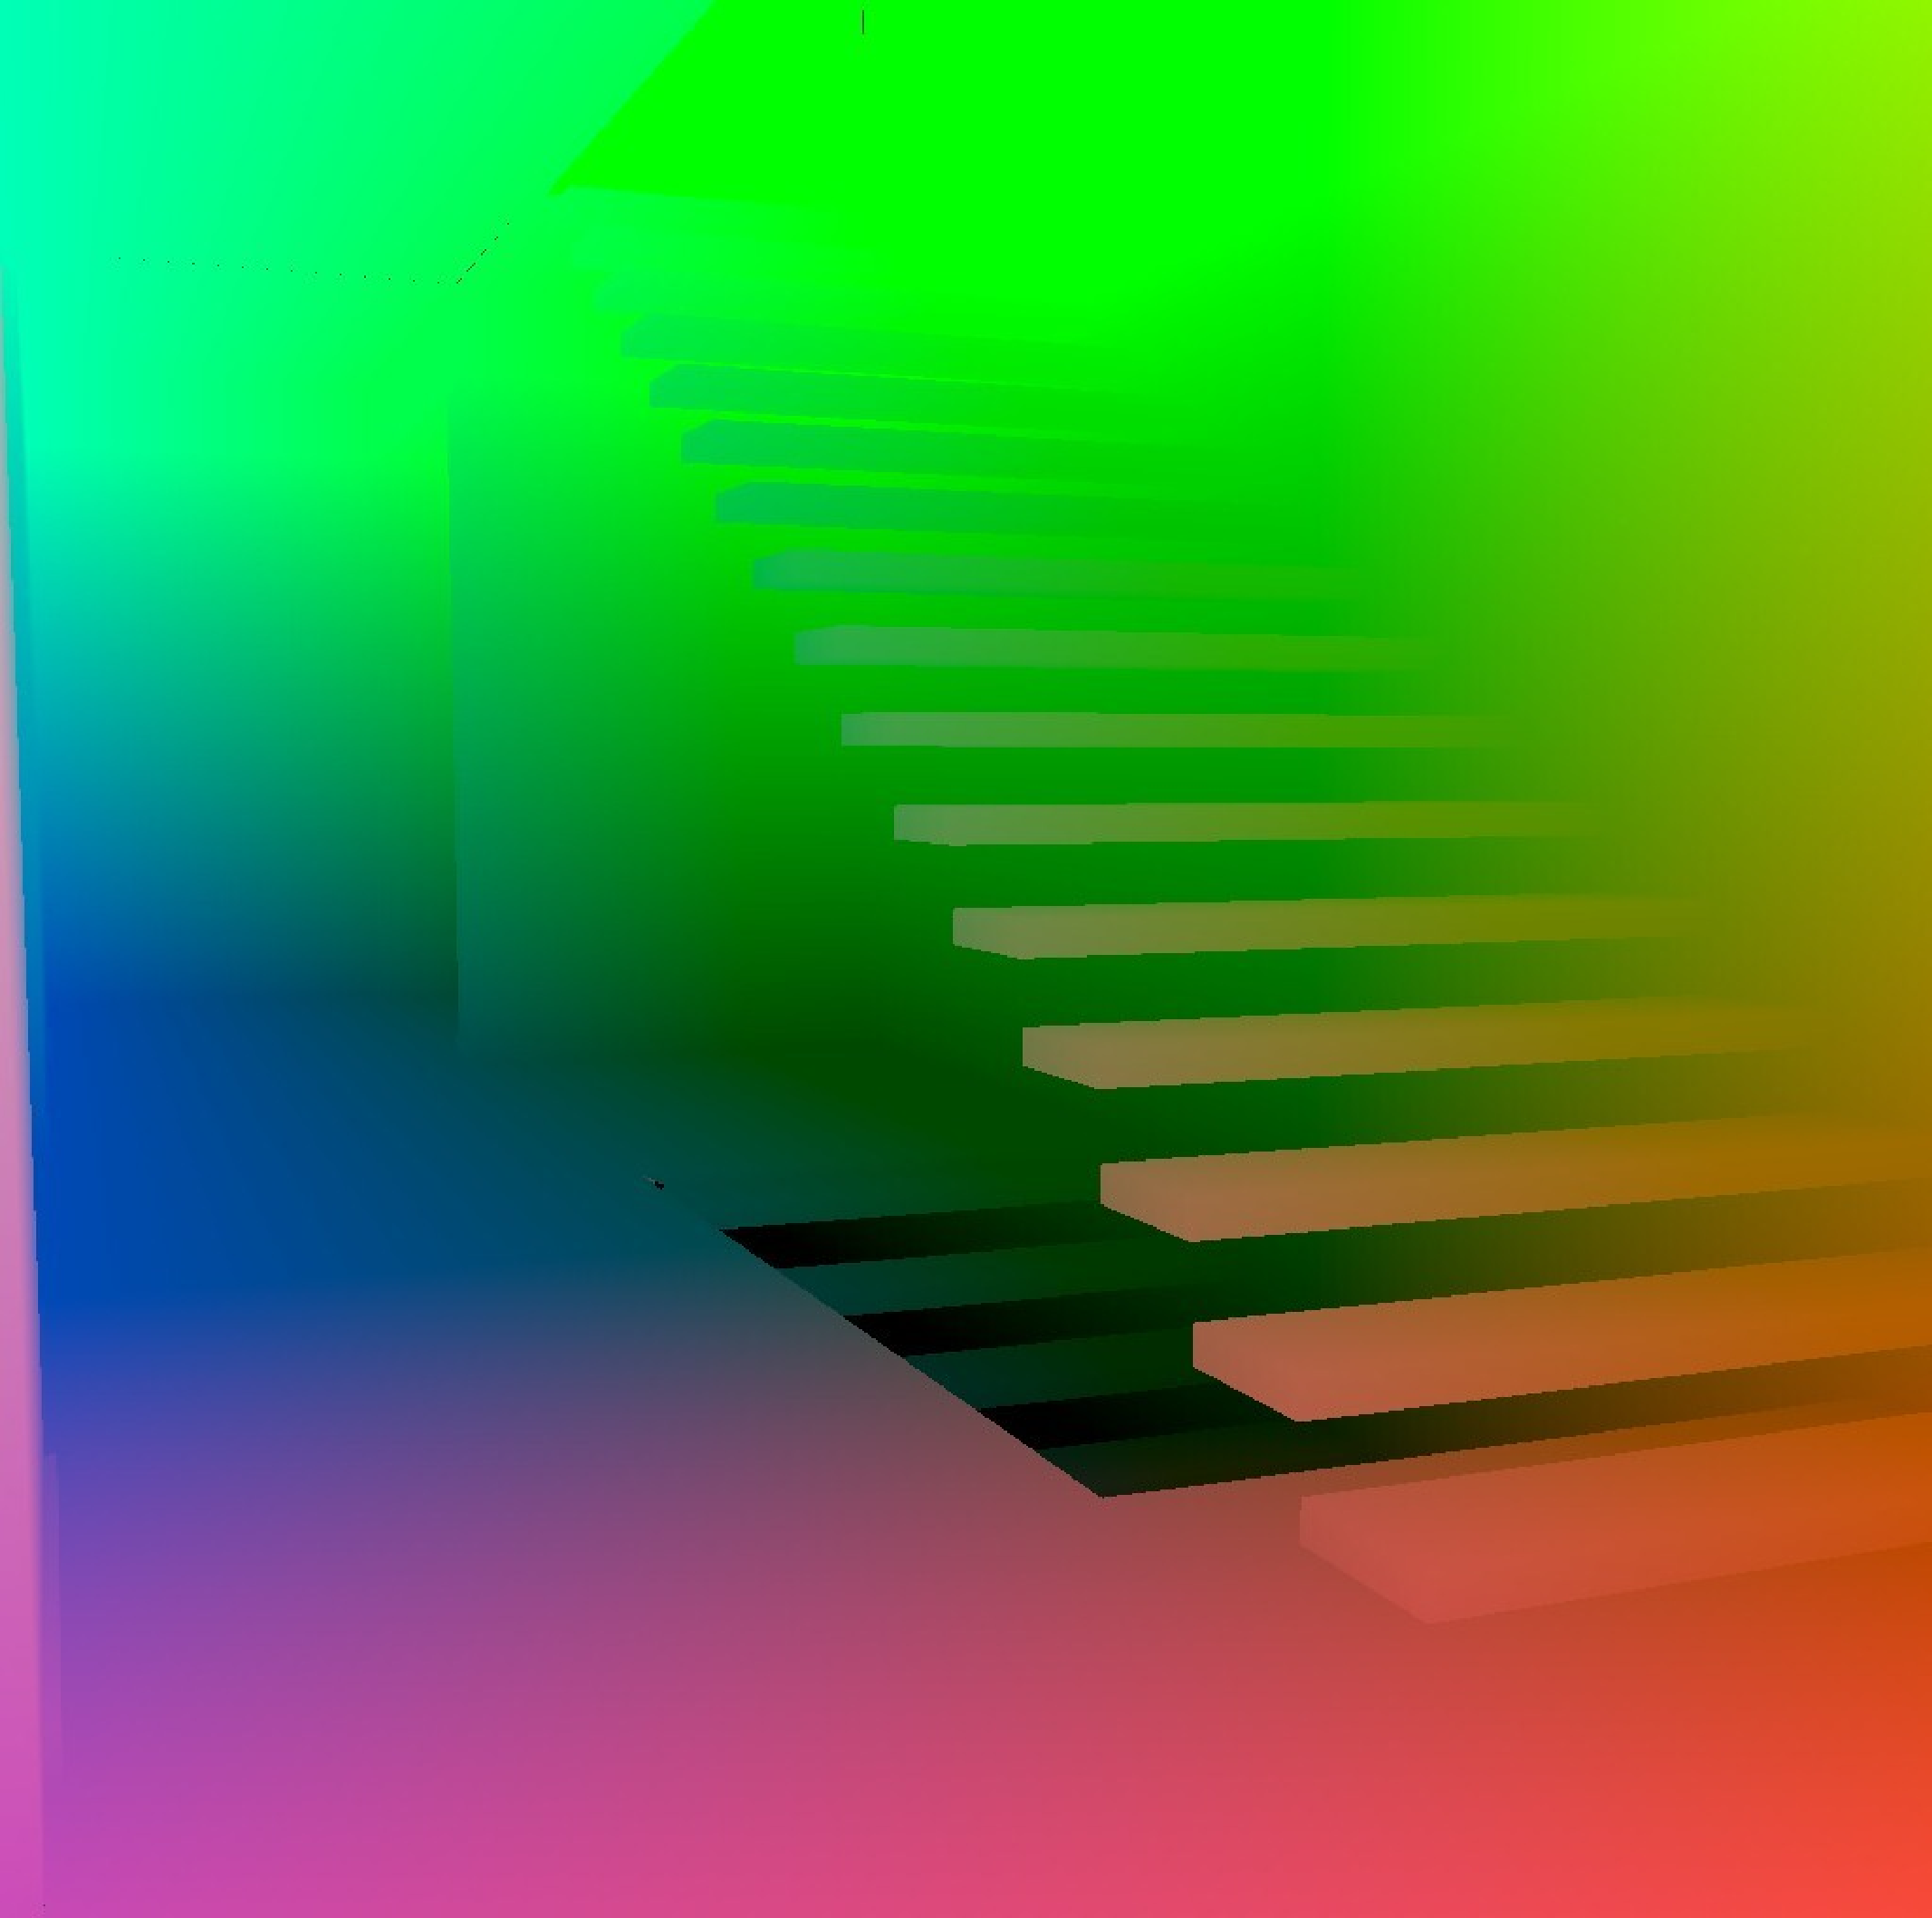
\includegraphics[width=\textwidth]{chapters/chapter_thetool/worldpos_scenepass1}
		\caption{World positions}
		\label{worldpos_scenepass1}
	\end{subfigure}
	\begin{subfigure}[t]{0.24\linewidth}
		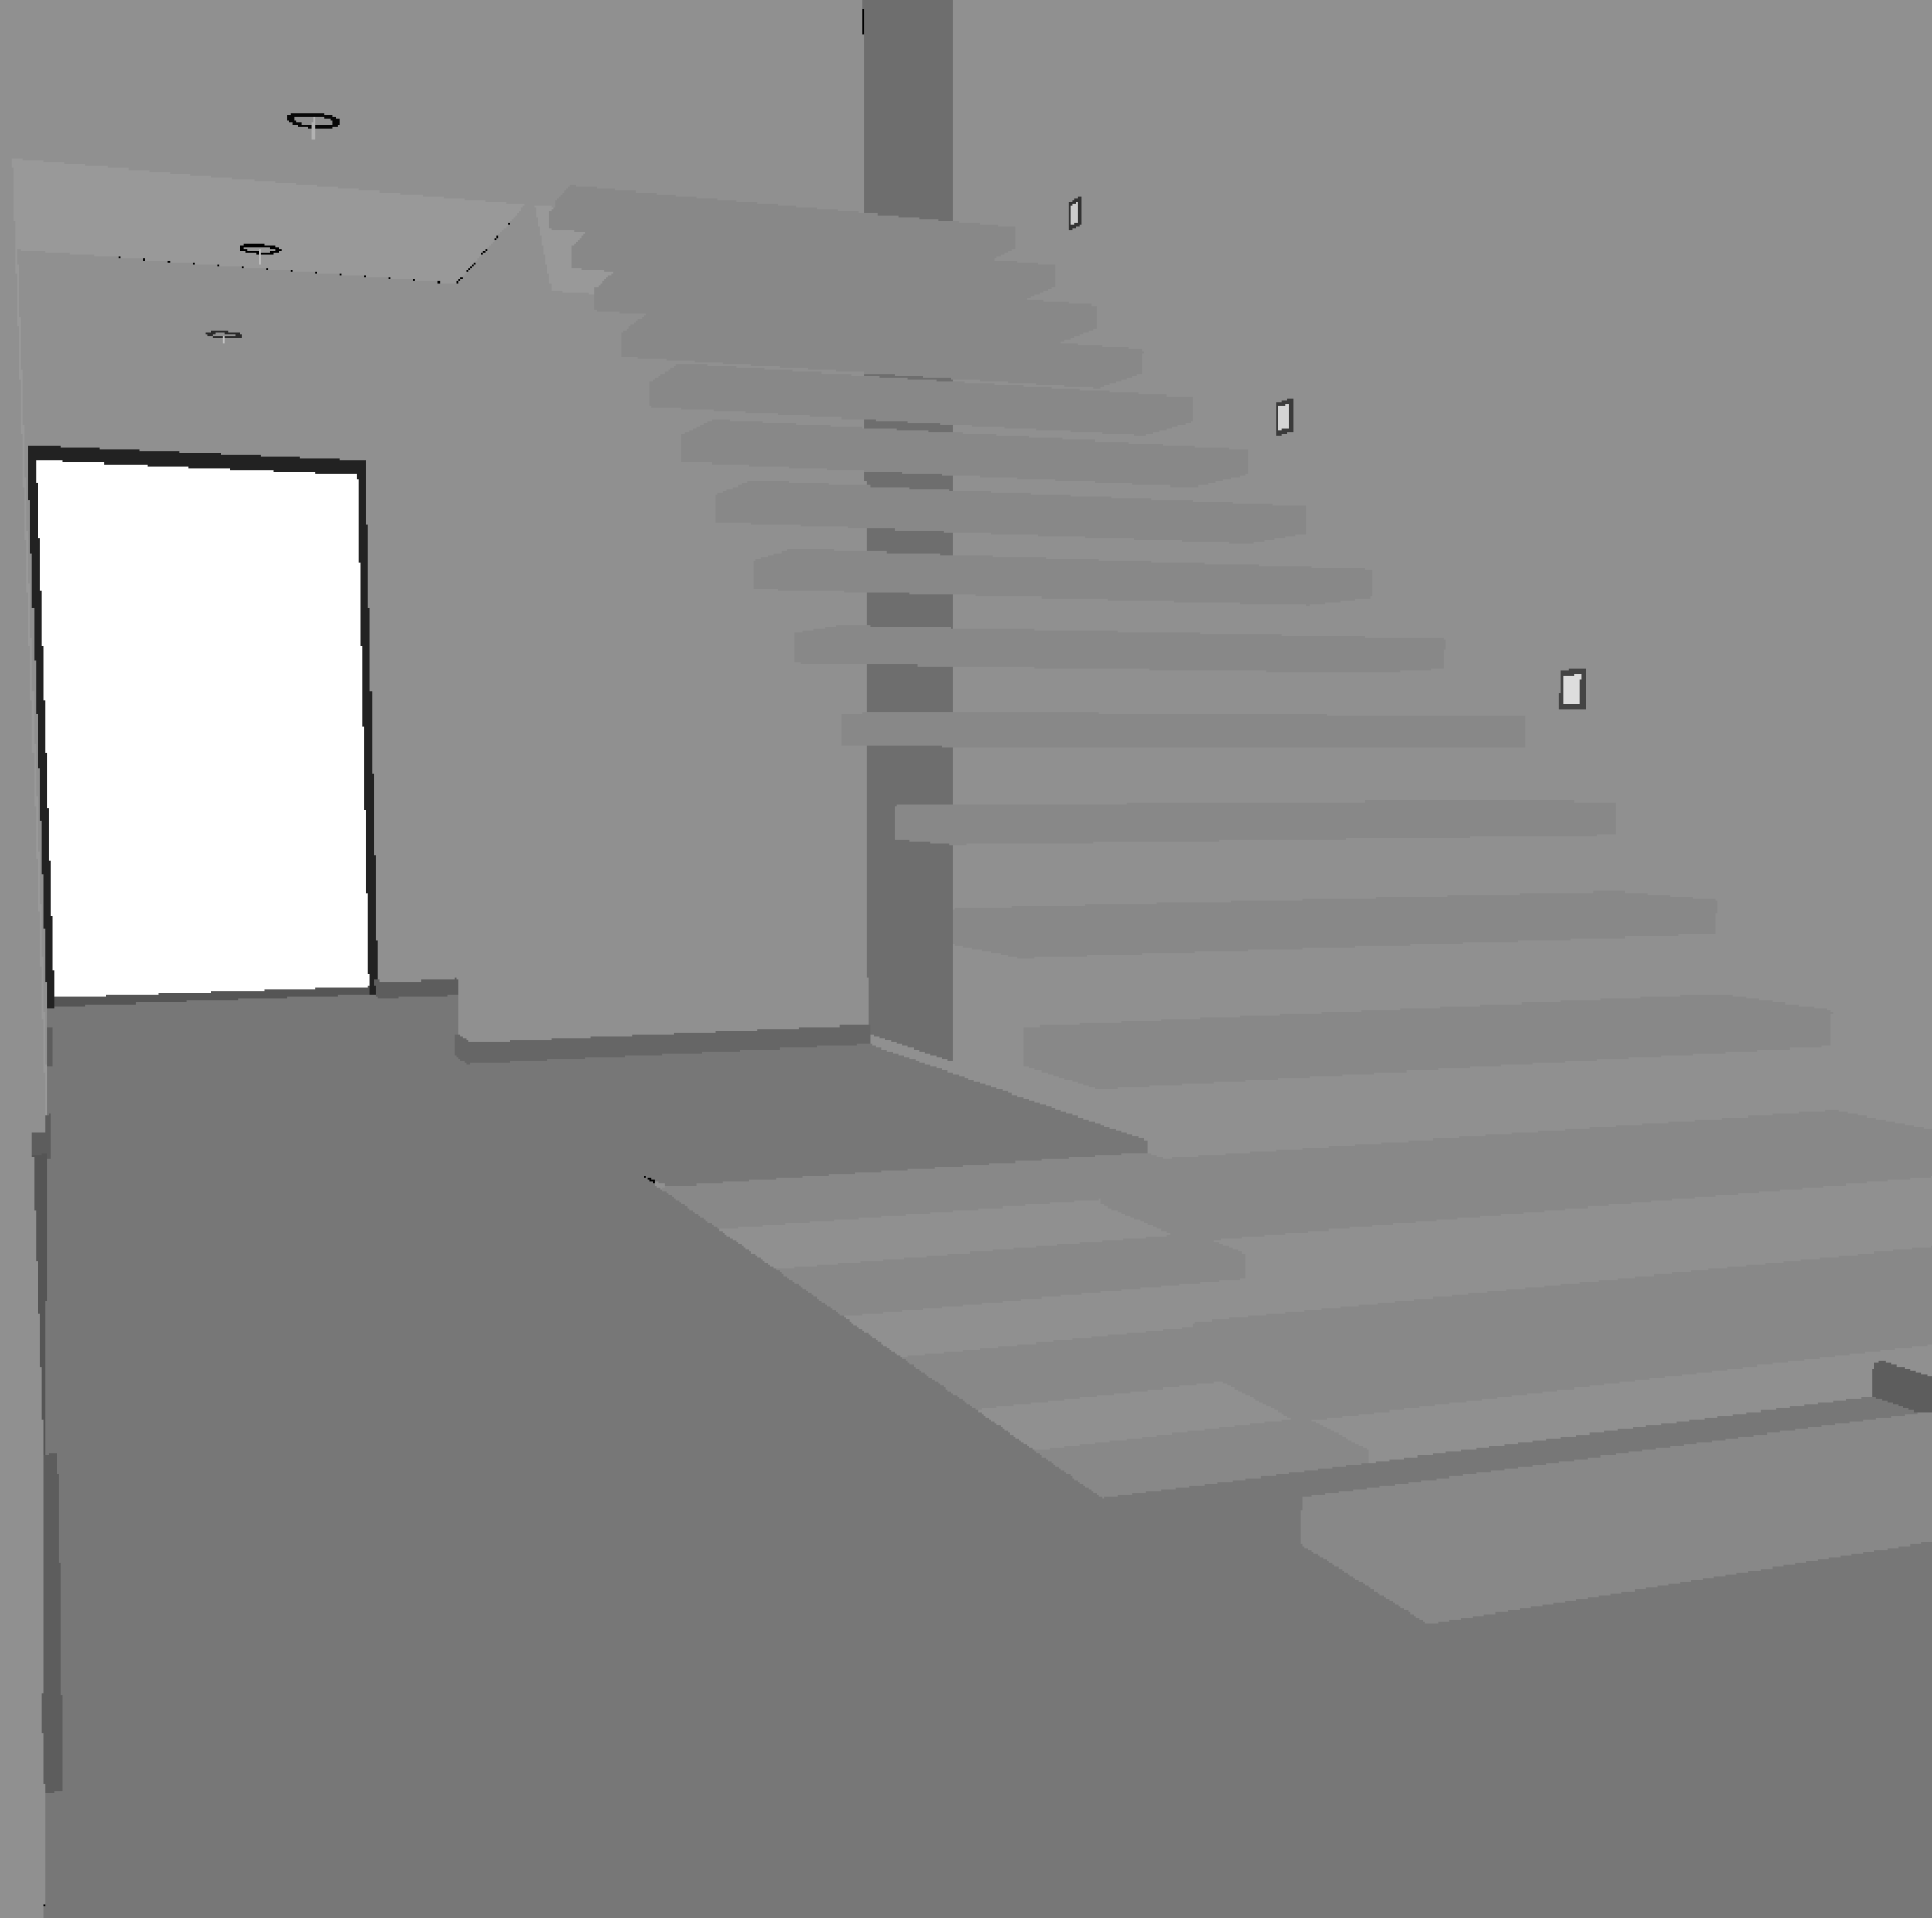
\includegraphics[width=\textwidth]{chapters/chapter_thetool/worldposa_scenepass1}
		\caption{Geometry ID}
		\label{worldposa_scenepass1}
	\end{subfigure}
	\begin{subfigure}[t]{0.24\linewidth}
		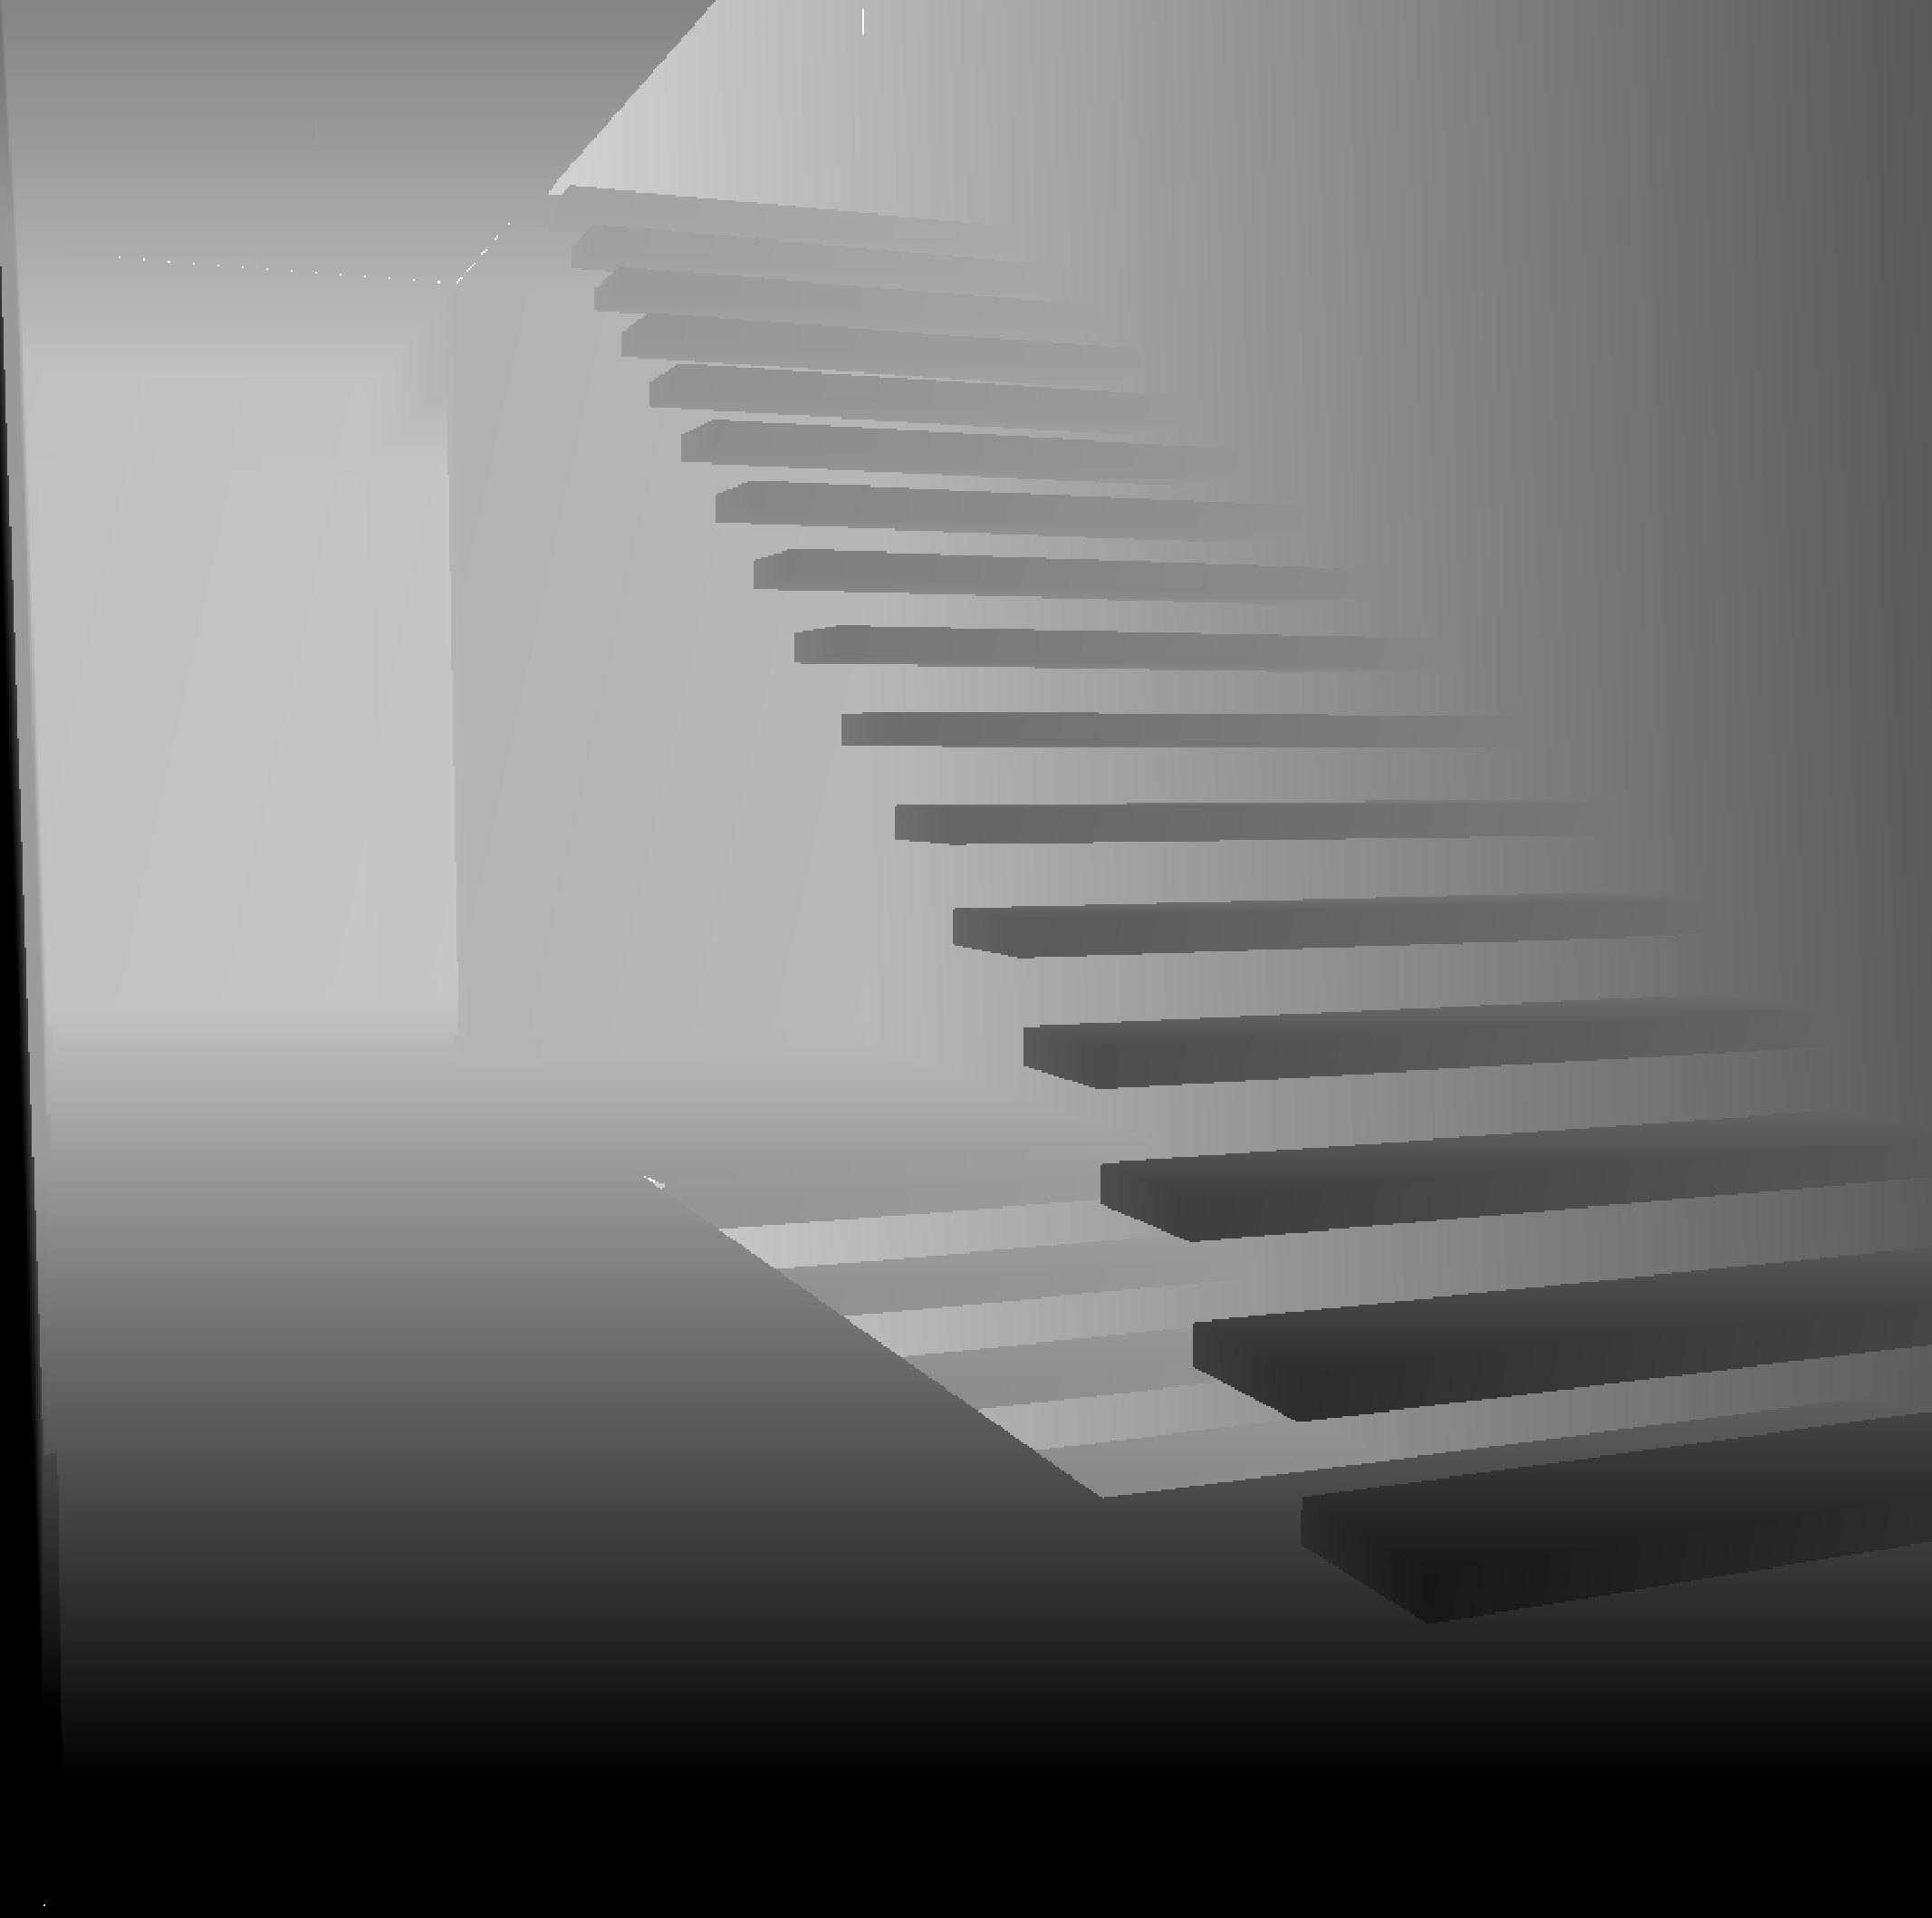
\includegraphics[width=\textwidth]{chapters/chapter_thetool/depth_scenepass1}
		\caption{Depth}
		\label{depth_scenepass1}
	\end{subfigure}

	\caption{Textures written by the opaque scene pass. The white and black levels of (b), (c) and (d) have been altered to improve readability.}
	\label{opaque_pass}
\end{figure}

The pass for translucent objects outputs beauty (fig. \ref{beauty_scenepass2}), world positions (fig. \ref{worldpos_scenepass2}), geometry IDs (fig. \ref{worldposa_scenepass2}), and depth (fig. \ref{depth_scenepass2}) as much as the previous pass does. Here though, while beauty and depth are written on new textures, the world positions and the geometries IDs are written upon the ones that came from the opaque pass (fig. \ref{worldpos_scenepass1} and \ref{worldposa_scenepass1}). Depth testing is enabled for this pass and it is performed against the depth texture of the opaque pass (fig. \ref{depth_scenepass1}); translucent objects behind opaque ones are simply not visible.

\begin{figure}
	\centering
	\begin{subfigure}[t]{0.24\linewidth}
		
\includegraphics[width=\textwidth]{chapters/chapter_thetool/beauty_scenepass2}
		\caption{Beauty}
		\label{beauty_scenepass2}
	\end{subfigure}
	\begin{subfigure}[t]{0.24\linewidth}
		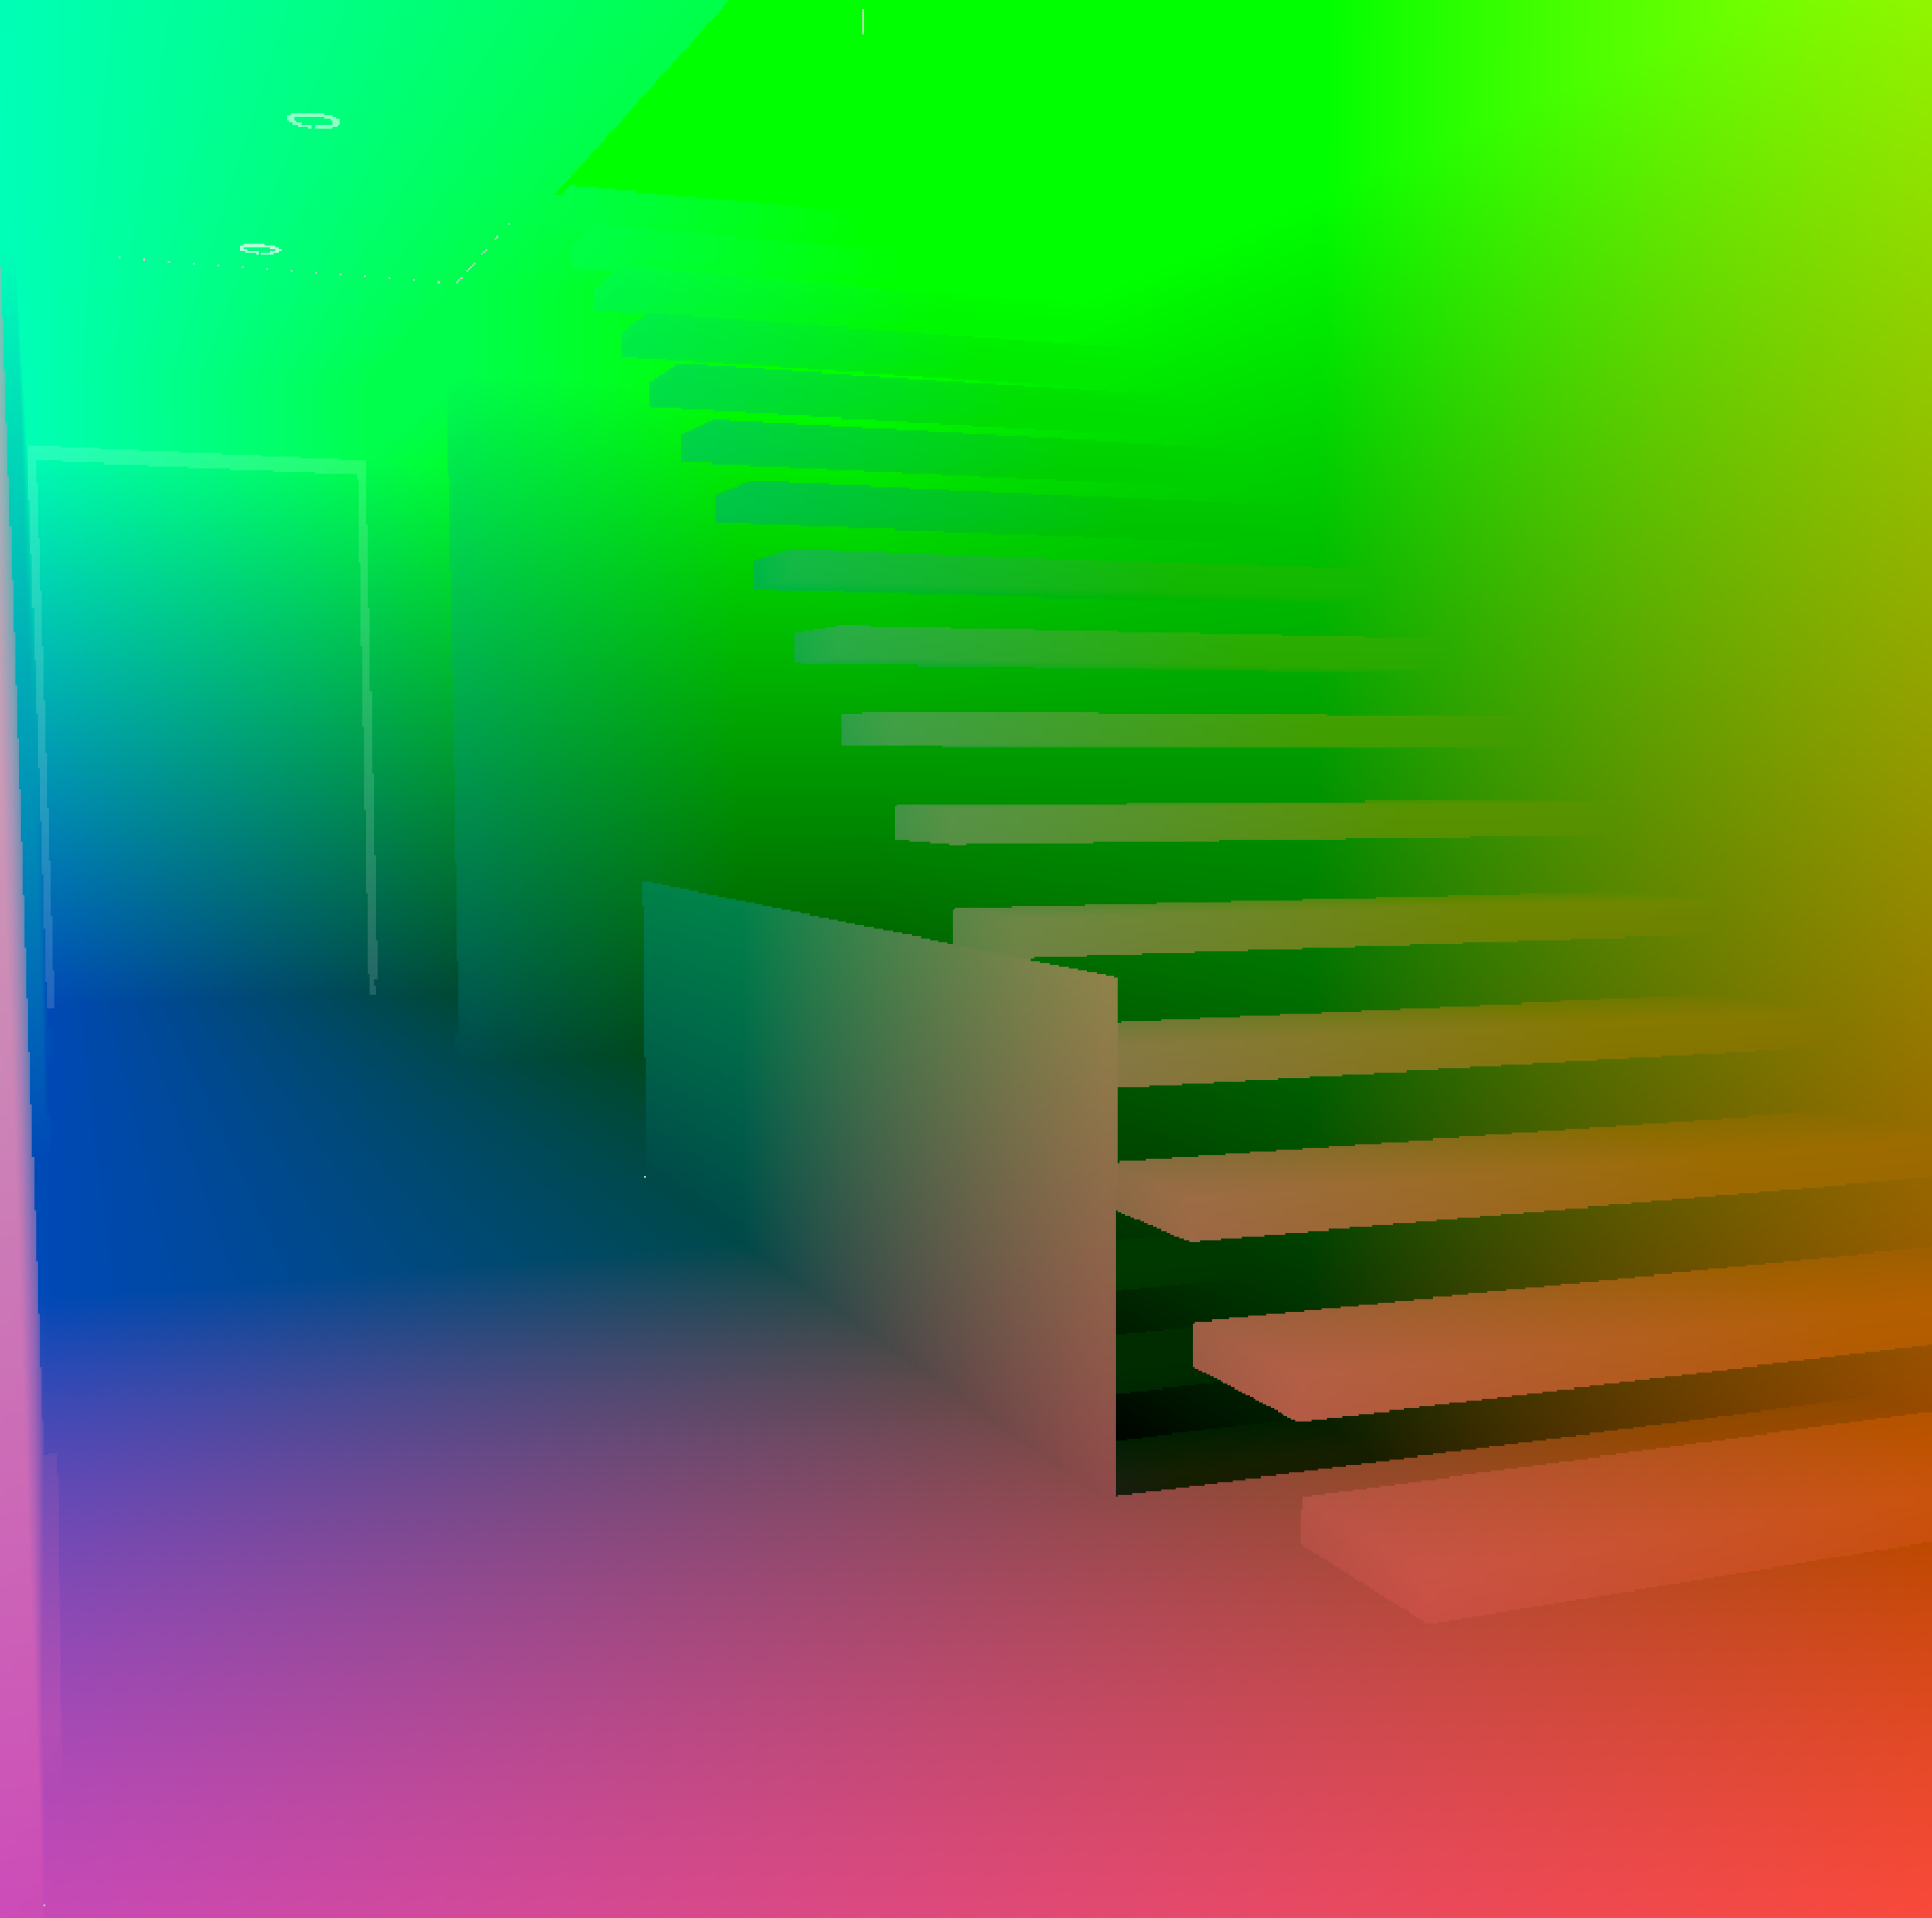
\includegraphics[width=\textwidth]{chapters/chapter_thetool/worldpos_scenepass2}
		\caption{World positions}
		\label{worldpos_scenepass2}
	\end{subfigure}
	\begin{subfigure}[t]{0.24\linewidth}
		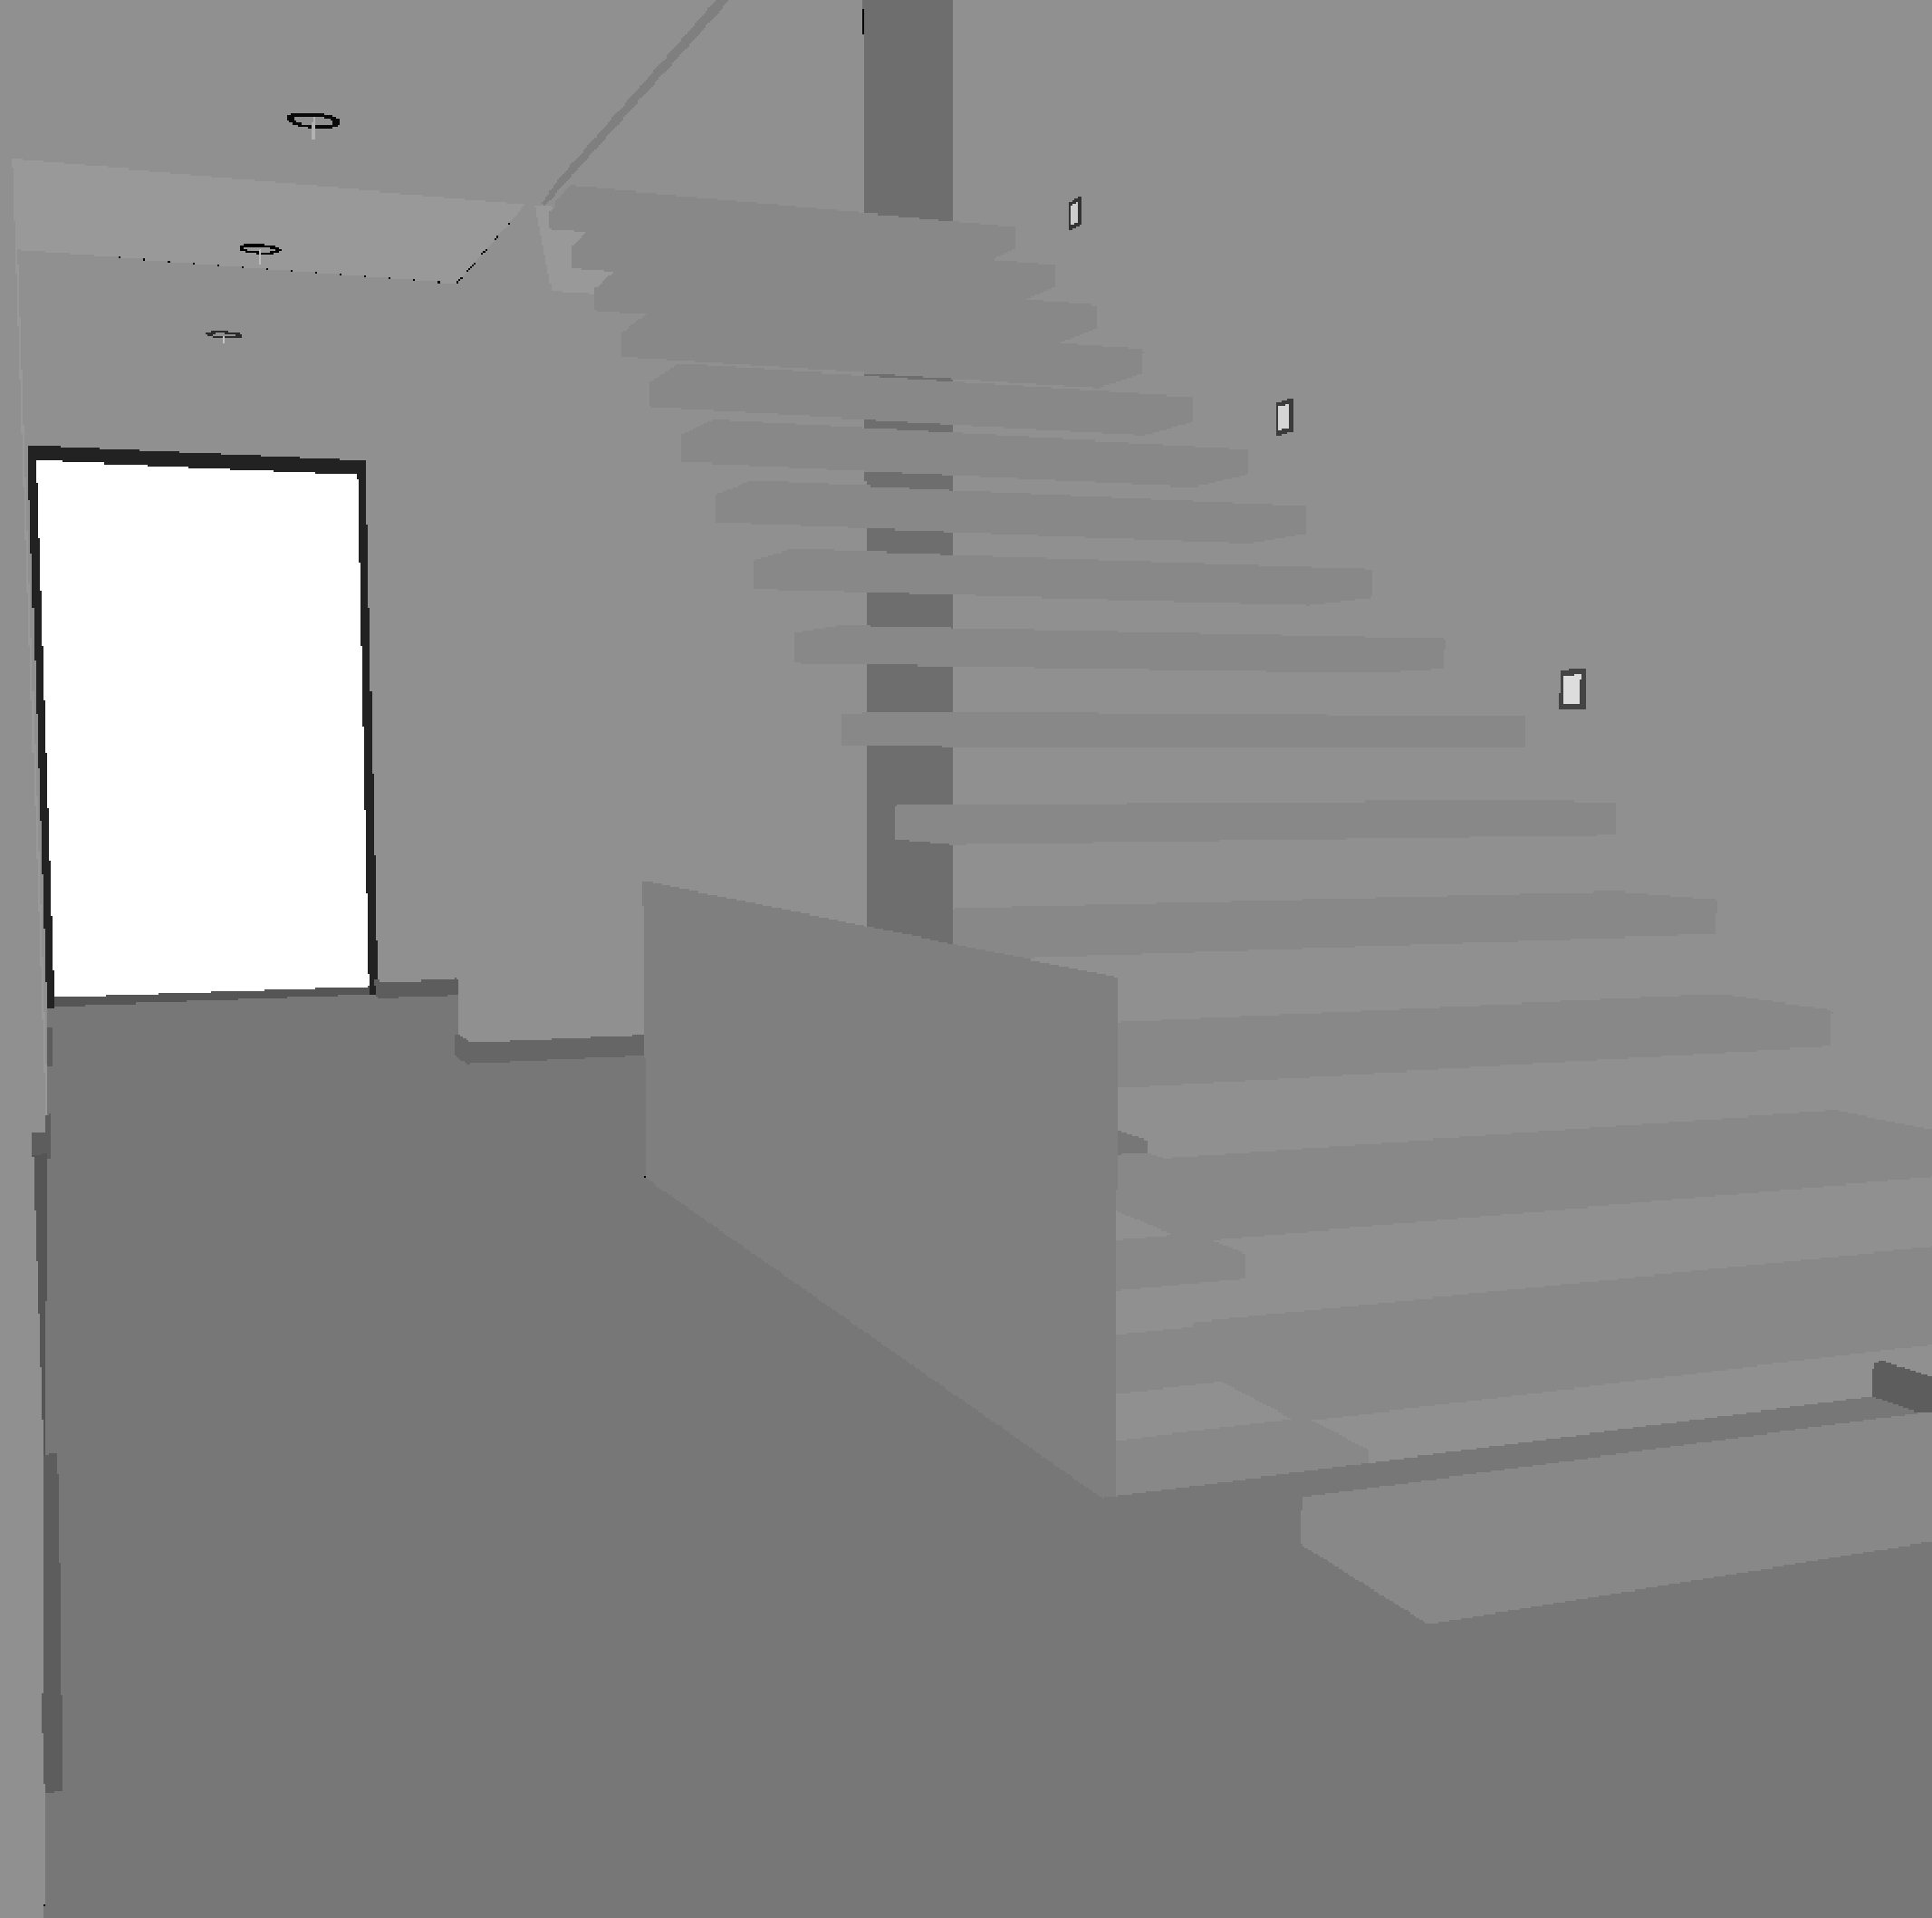
\includegraphics[width=\textwidth]{chapters/chapter_thetool/worldposa_scenepass2}
		\caption{Geometry ID}
		\label{worldposa_scenepass2}
	\end{subfigure}
	\begin{subfigure}[t]{0.24\linewidth}
		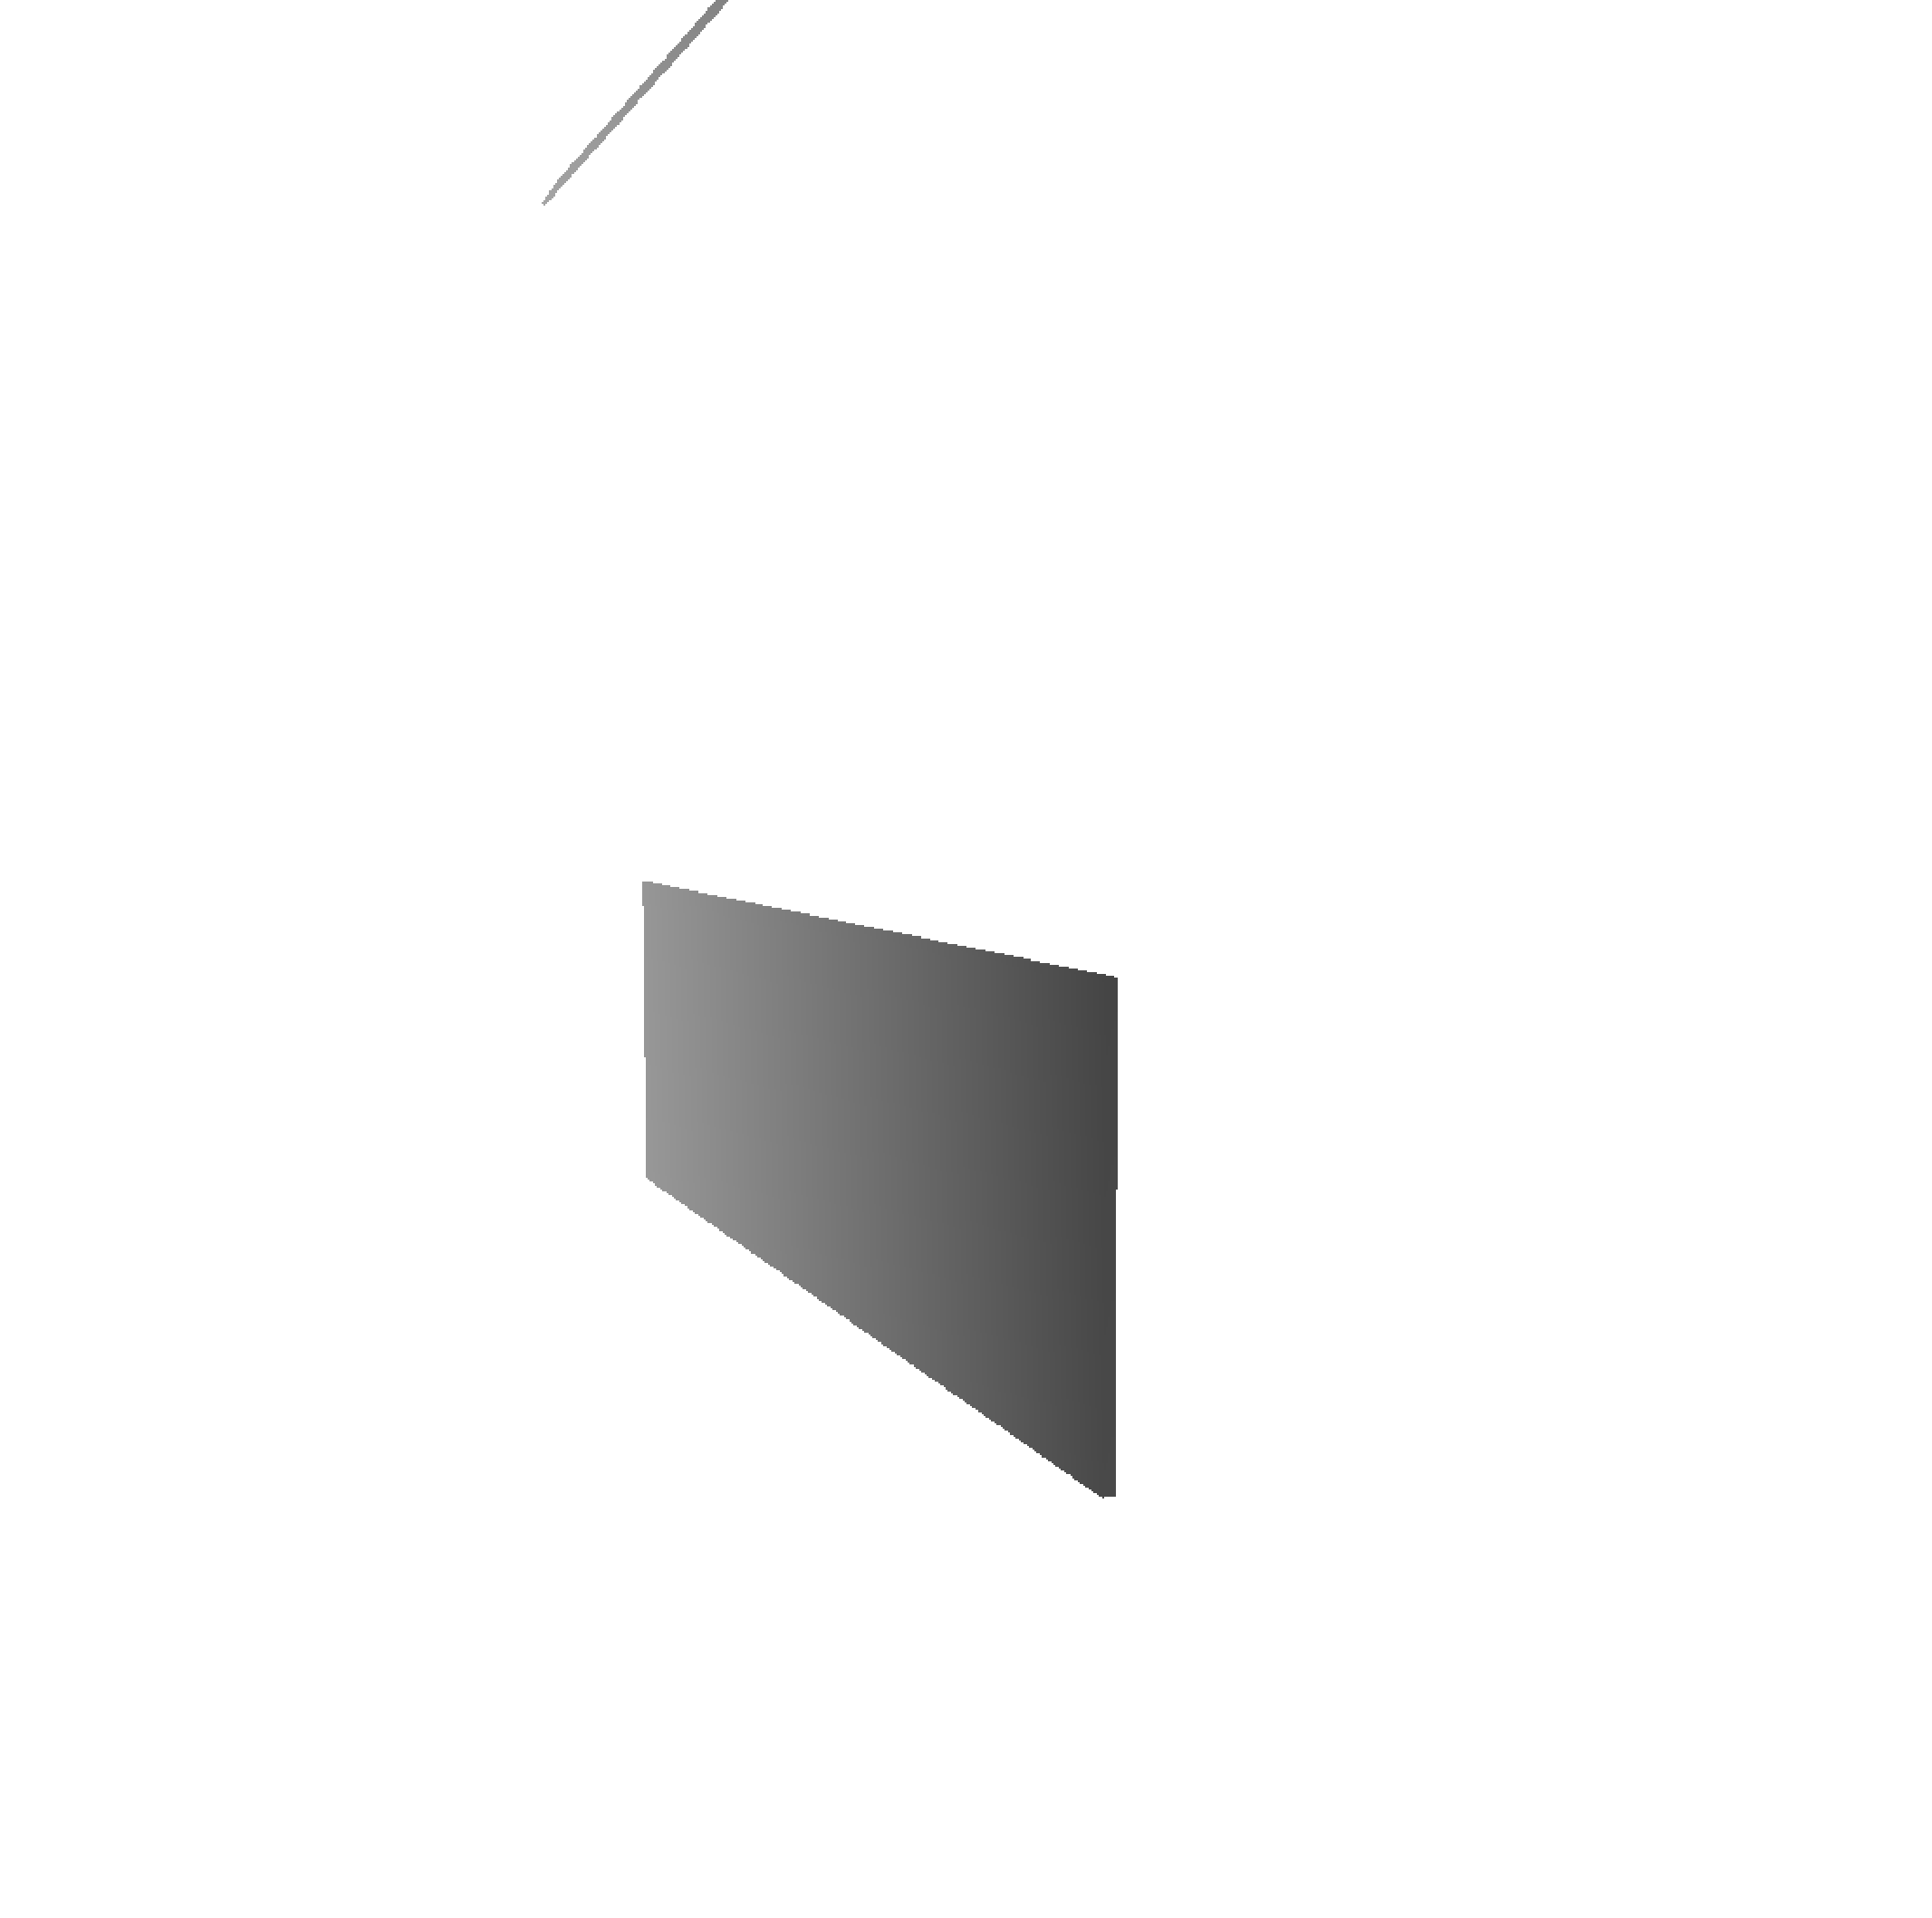
\includegraphics[width=\textwidth]{chapters/chapter_thetool/depth_scenepass2}
		\caption{Depth}
		\label{depth_scenepass2}
	\end{subfigure}

	\caption{Textures written by the translucent scene pass. The white and black levels of (b), (c) and (d) have been altered to improve readability.}
	\label{translucent_pass}
\end{figure}

To facilitate scene navigation and readability, some visualization options are provided under the \textbf{“Scene”} section of the \textbf{“Visualization options”} panel:
\begin{description}
	\item[“Blend color”/“Blend alpha”] They perform alpha blending of the fragments of the scene with the user specified color; it comes in handy when a scene has many bright-colored surfaces which can make paths difficult to see. A visual example is provided in figure \ref{blendcolor_fig}.
	\item[“Geometries”] This collapsible section lets the user toggle visibility and back face culling for either single geometries or all of them together. Users can click on a geometry from the viewport to select it. A selected geometry will be rendered in yellow by the viewport and its name on the \textbf{“Geometries”} list will be highlighted. Geometries can be selected from the list too.
	\item[“Heatmap”] It enables the bounce density heatmap rendering, feature described extensively in section \ref{heatmap}.
\end{description}

\begin{figure}
	\centering
	\begin{subfigure}[t]{0.49\linewidth}
		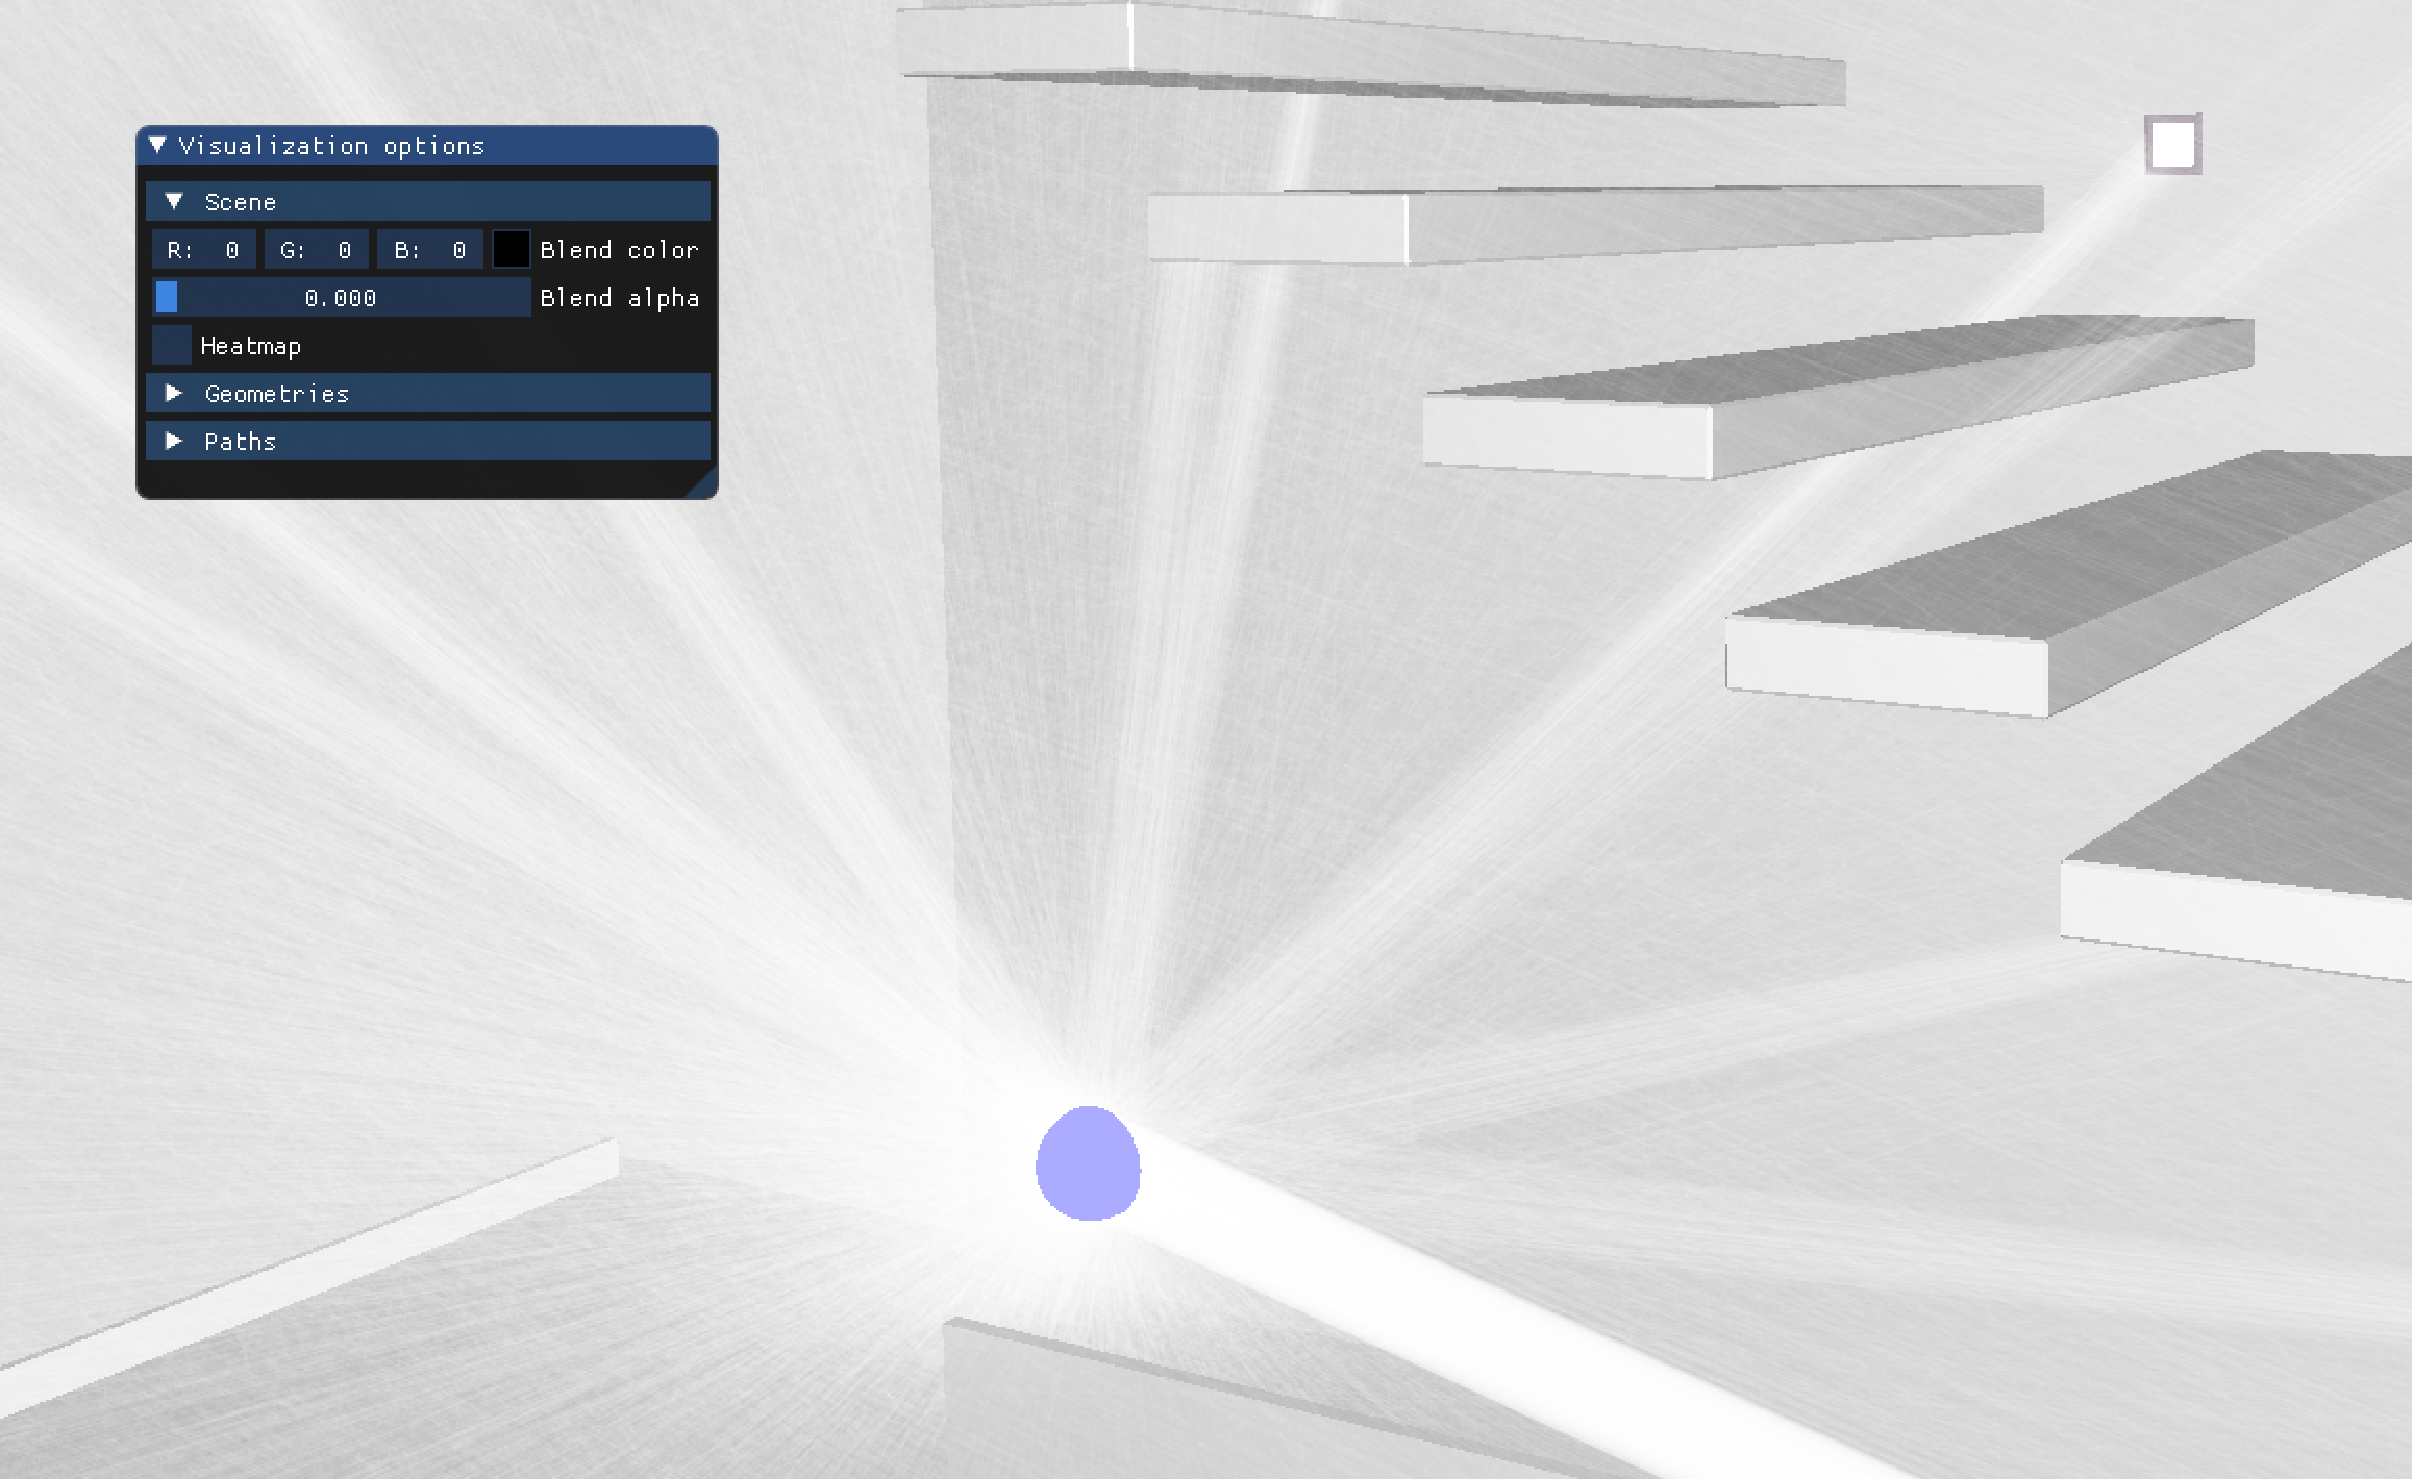
\includegraphics[width=\textwidth]{chapters/chapter_thetool/blendcolor_before}
		\caption{Alpha $= 0$}
	\end{subfigure}
	\begin{subfigure}[t]{0.49\linewidth}
		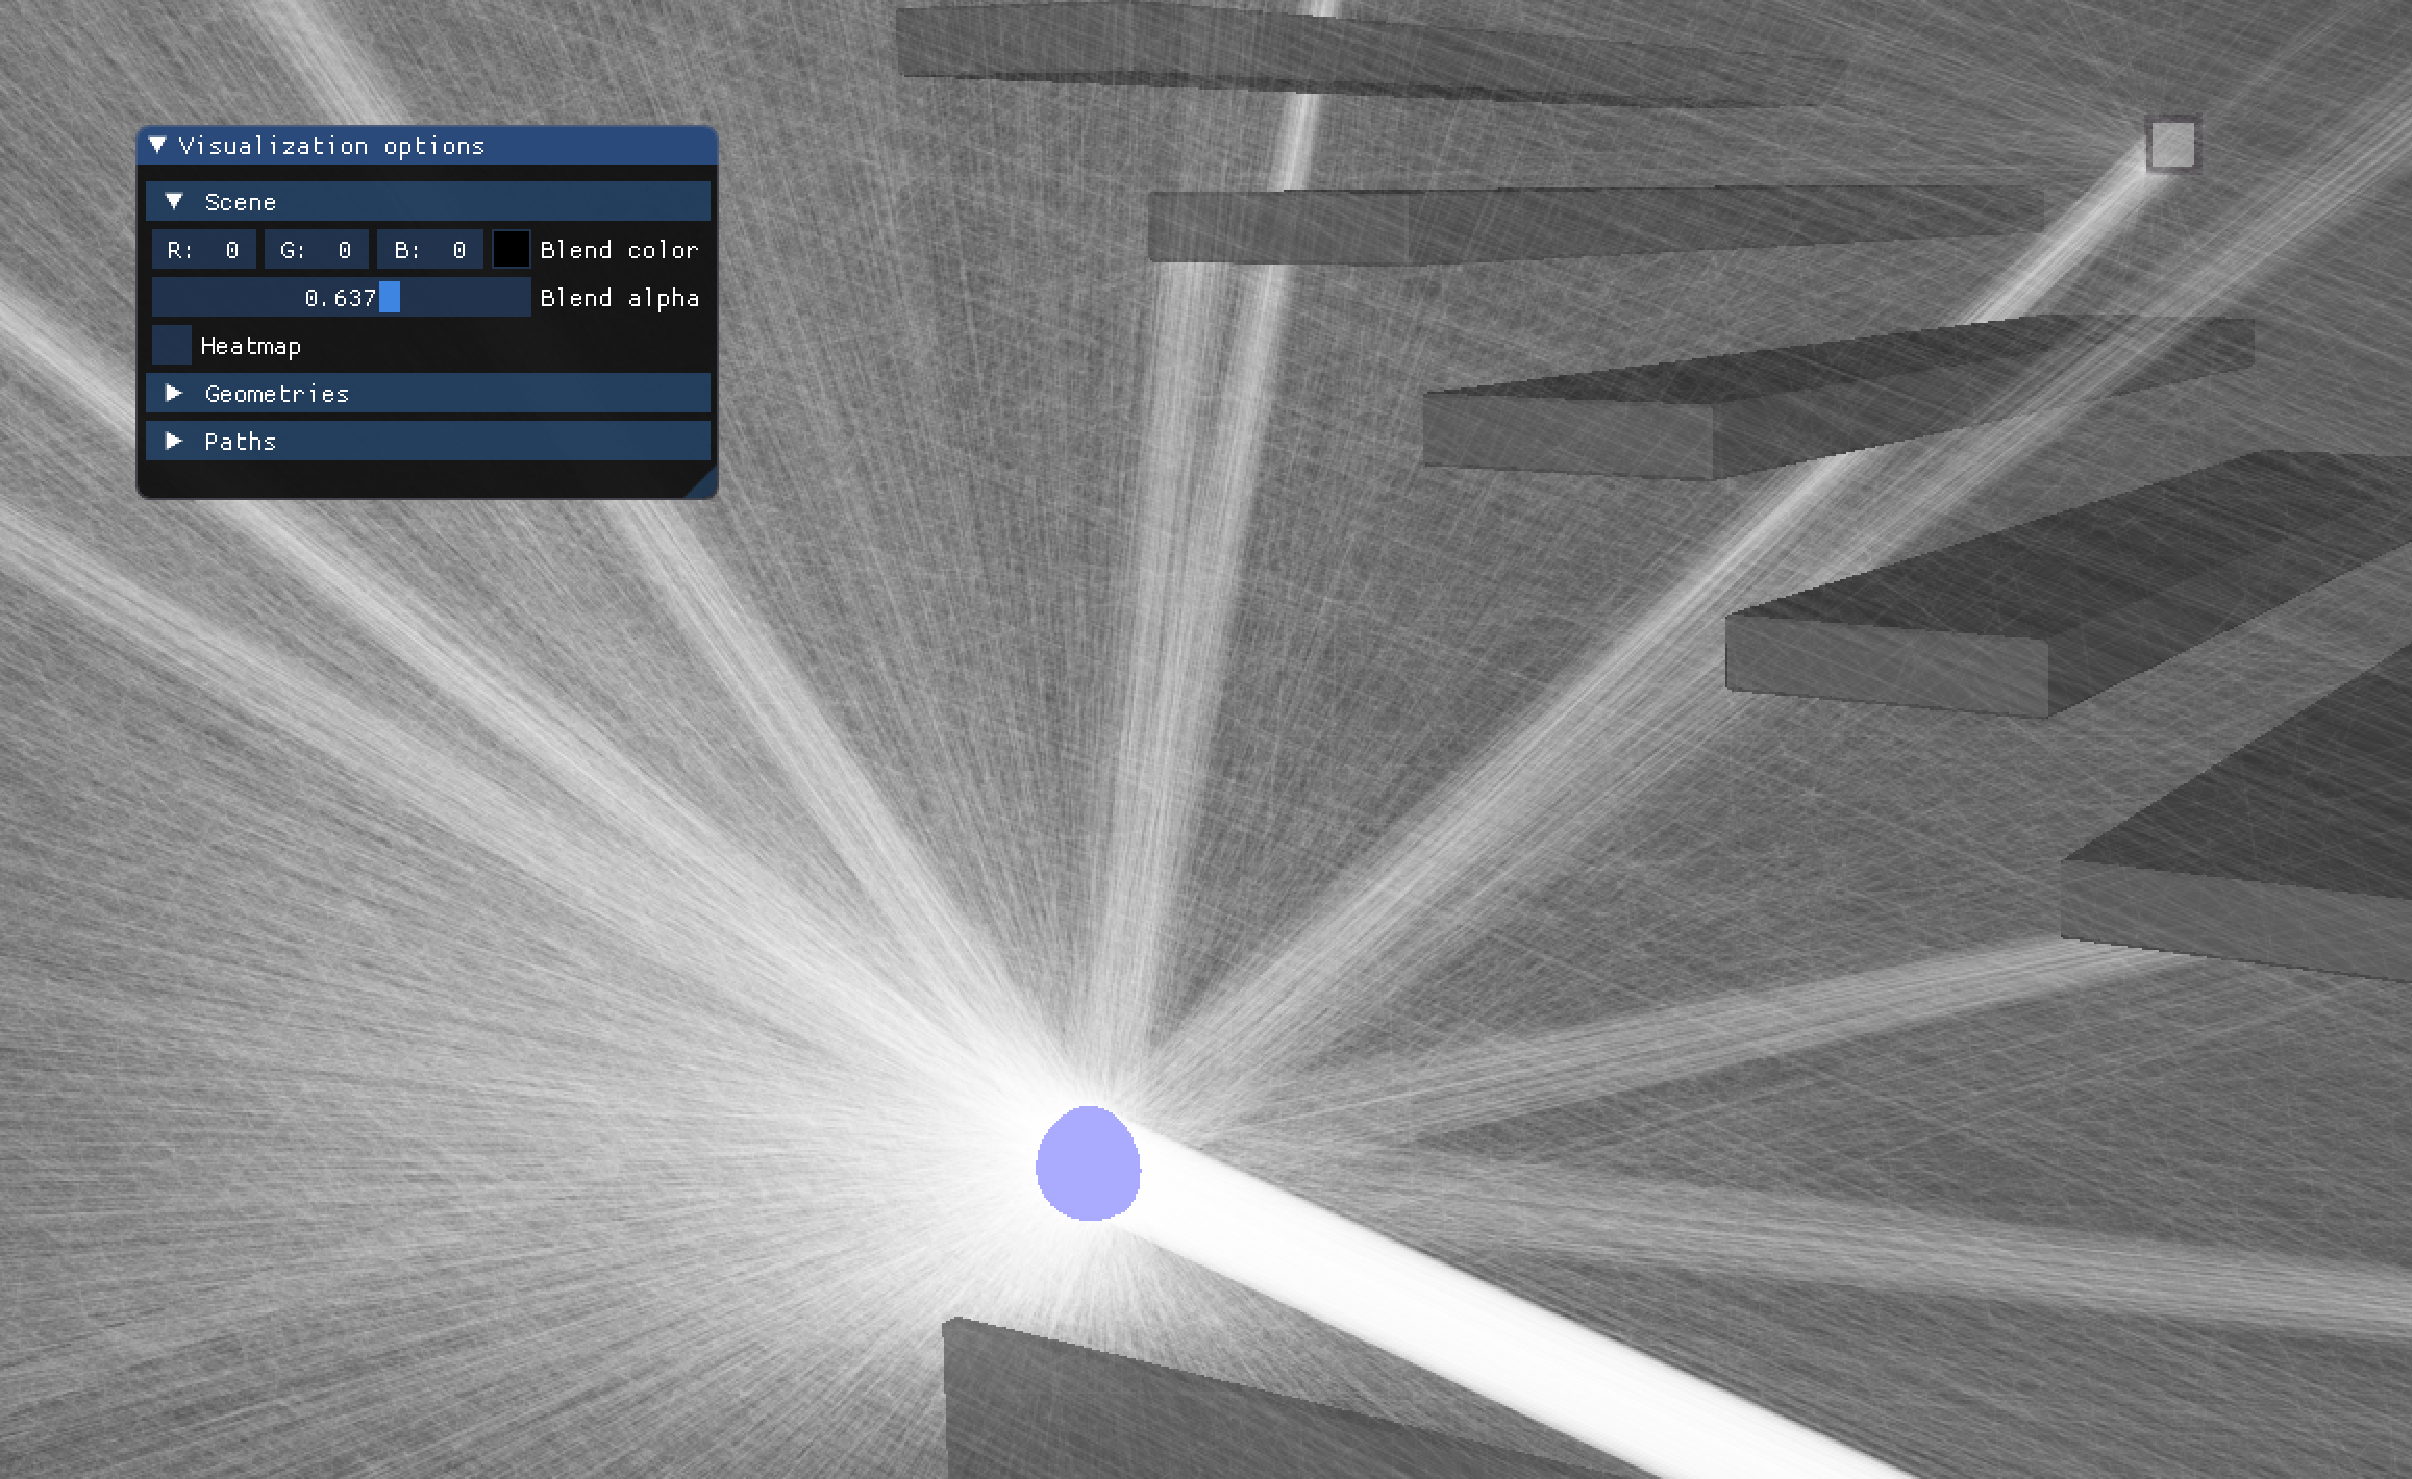
\includegraphics[width=\textwidth]{chapters/chapter_thetool/blendcolor_after}
		\caption{Alpha $= 0.637$}
	\end{subfigure}

	\caption{Use of the blend color visualization option to improve path visibility in a bright scene.}
	\label{blendcolor_fig}
\end{figure}

Right after the scene passes, the paths are rendered. Every time there is a change of the set of the selected paths, the new set is loaded on the GPU. The rendering is done using the \texttt{glMultiDrawArrays} OpenGL render function with the \texttt{GL\_LINE\_STRIP} render mode. This has been proven to be visibly faster than calling \texttt{glDrawArrays} several times inside a \texttt{for} loop. Through the use of the two depth textures generated by the scene render passes (fig. \ref{depth_scenepass1} and \ref{depth_scenepass2}), the path fragments are rendered on two textures: a \textit{front} (fig. \ref{rays_front}) and a \textit{back} (fig. \ref{rays_back}) one. All the fragments that are occluded by neither opaque nor translucent scene geometry end up in the front texture, the ones occluded only by a translucent geometry fill the back texture. Since usually hundreds of thousands of paths pass through a single pixel, the OpenGL built-in alpha blending is enabled. By default, all paths are rasterized with an alpha value directly controlled by the \textbf{“Paths alpha”} slider on the \textbf{“Paths”} section of the \textbf{“Visualization options”} panel. In that section there are also three checkboxes controlling other visual properties of the paths:
\begin{description}
	\item[“Render”] Toggles the rendering of the paths all together. It might be helpful in situations where the user selected too many paths and moving the viewport camera gets difficult.
	\item[“Depth test”] Toggles the depth test during paths' rendering. It can be handy with cluttered scenes.
	\item[“Radiance scaling”] When checked, the paths' alpha gets scaled by their transported radiance. In other words, it gives a visual method to pick the rays that carry more light energy than others. This can be useful while determining the origin of fireflies and such rendering artifacts. From the implementation point of view, this is achieved by loading to the GPU a shader storage buffer --- \texttt{sso} for short --- containing the summed radiance of the red, green and blue channels of each path; the shaders then, thanks to the \texttt{gl\_DrawID} variable --- which is available since the \texttt{glMultiDrawArrays} render function is used ---, can access the \texttt{sso} correctly and shade the paths by multiplying the radiance with the user defined path alpha.
\end{description}

Reached this point, what the viewport rendered until now is composited together.
Starting from the opaque beauty texture (fig. \ref{beauty_scenepass1}), the \textit{back} paths are added (fig. \ref{rays_back}), then the translucent beauty texture (fig. \ref{beauty_scenepass2}) is alpha blended over with a default value of 0.7 and finally the \textit{front} paths (fig. \ref{rays_front}) are super imposed. This leads to the result shown in figure \ref{beauty+rays}. As probably already noticed by the reader, this render pipeline provides a rather simplistic way to solve the so often called “transparency problem” that breaks when there are paths that has to be rendered between two translucent objects: they will render as they were behind both objects. Due to the lesser severity of the resulting artifacts, a proper and technically more complex solution has never been even planned.

To make filters appear over the paths, they are rendered last. They are first rendered as a mask (fig. \ref{filter_mask}), taking in account only the opaque depth texture (fig. \ref{depth_scenepass1}) so that filters appear occluded by opaque object scenes. The mask is then used to composite the \textit{scene + paths} with a semi-transparent dark blue of RGBA value of $(0,0,0.33,0.33)$, outputting the final frame (fig. \ref{viewport_render}).

\begin{figure}
	\centering
	\begin{subfigure}[t]{0.24\linewidth}
		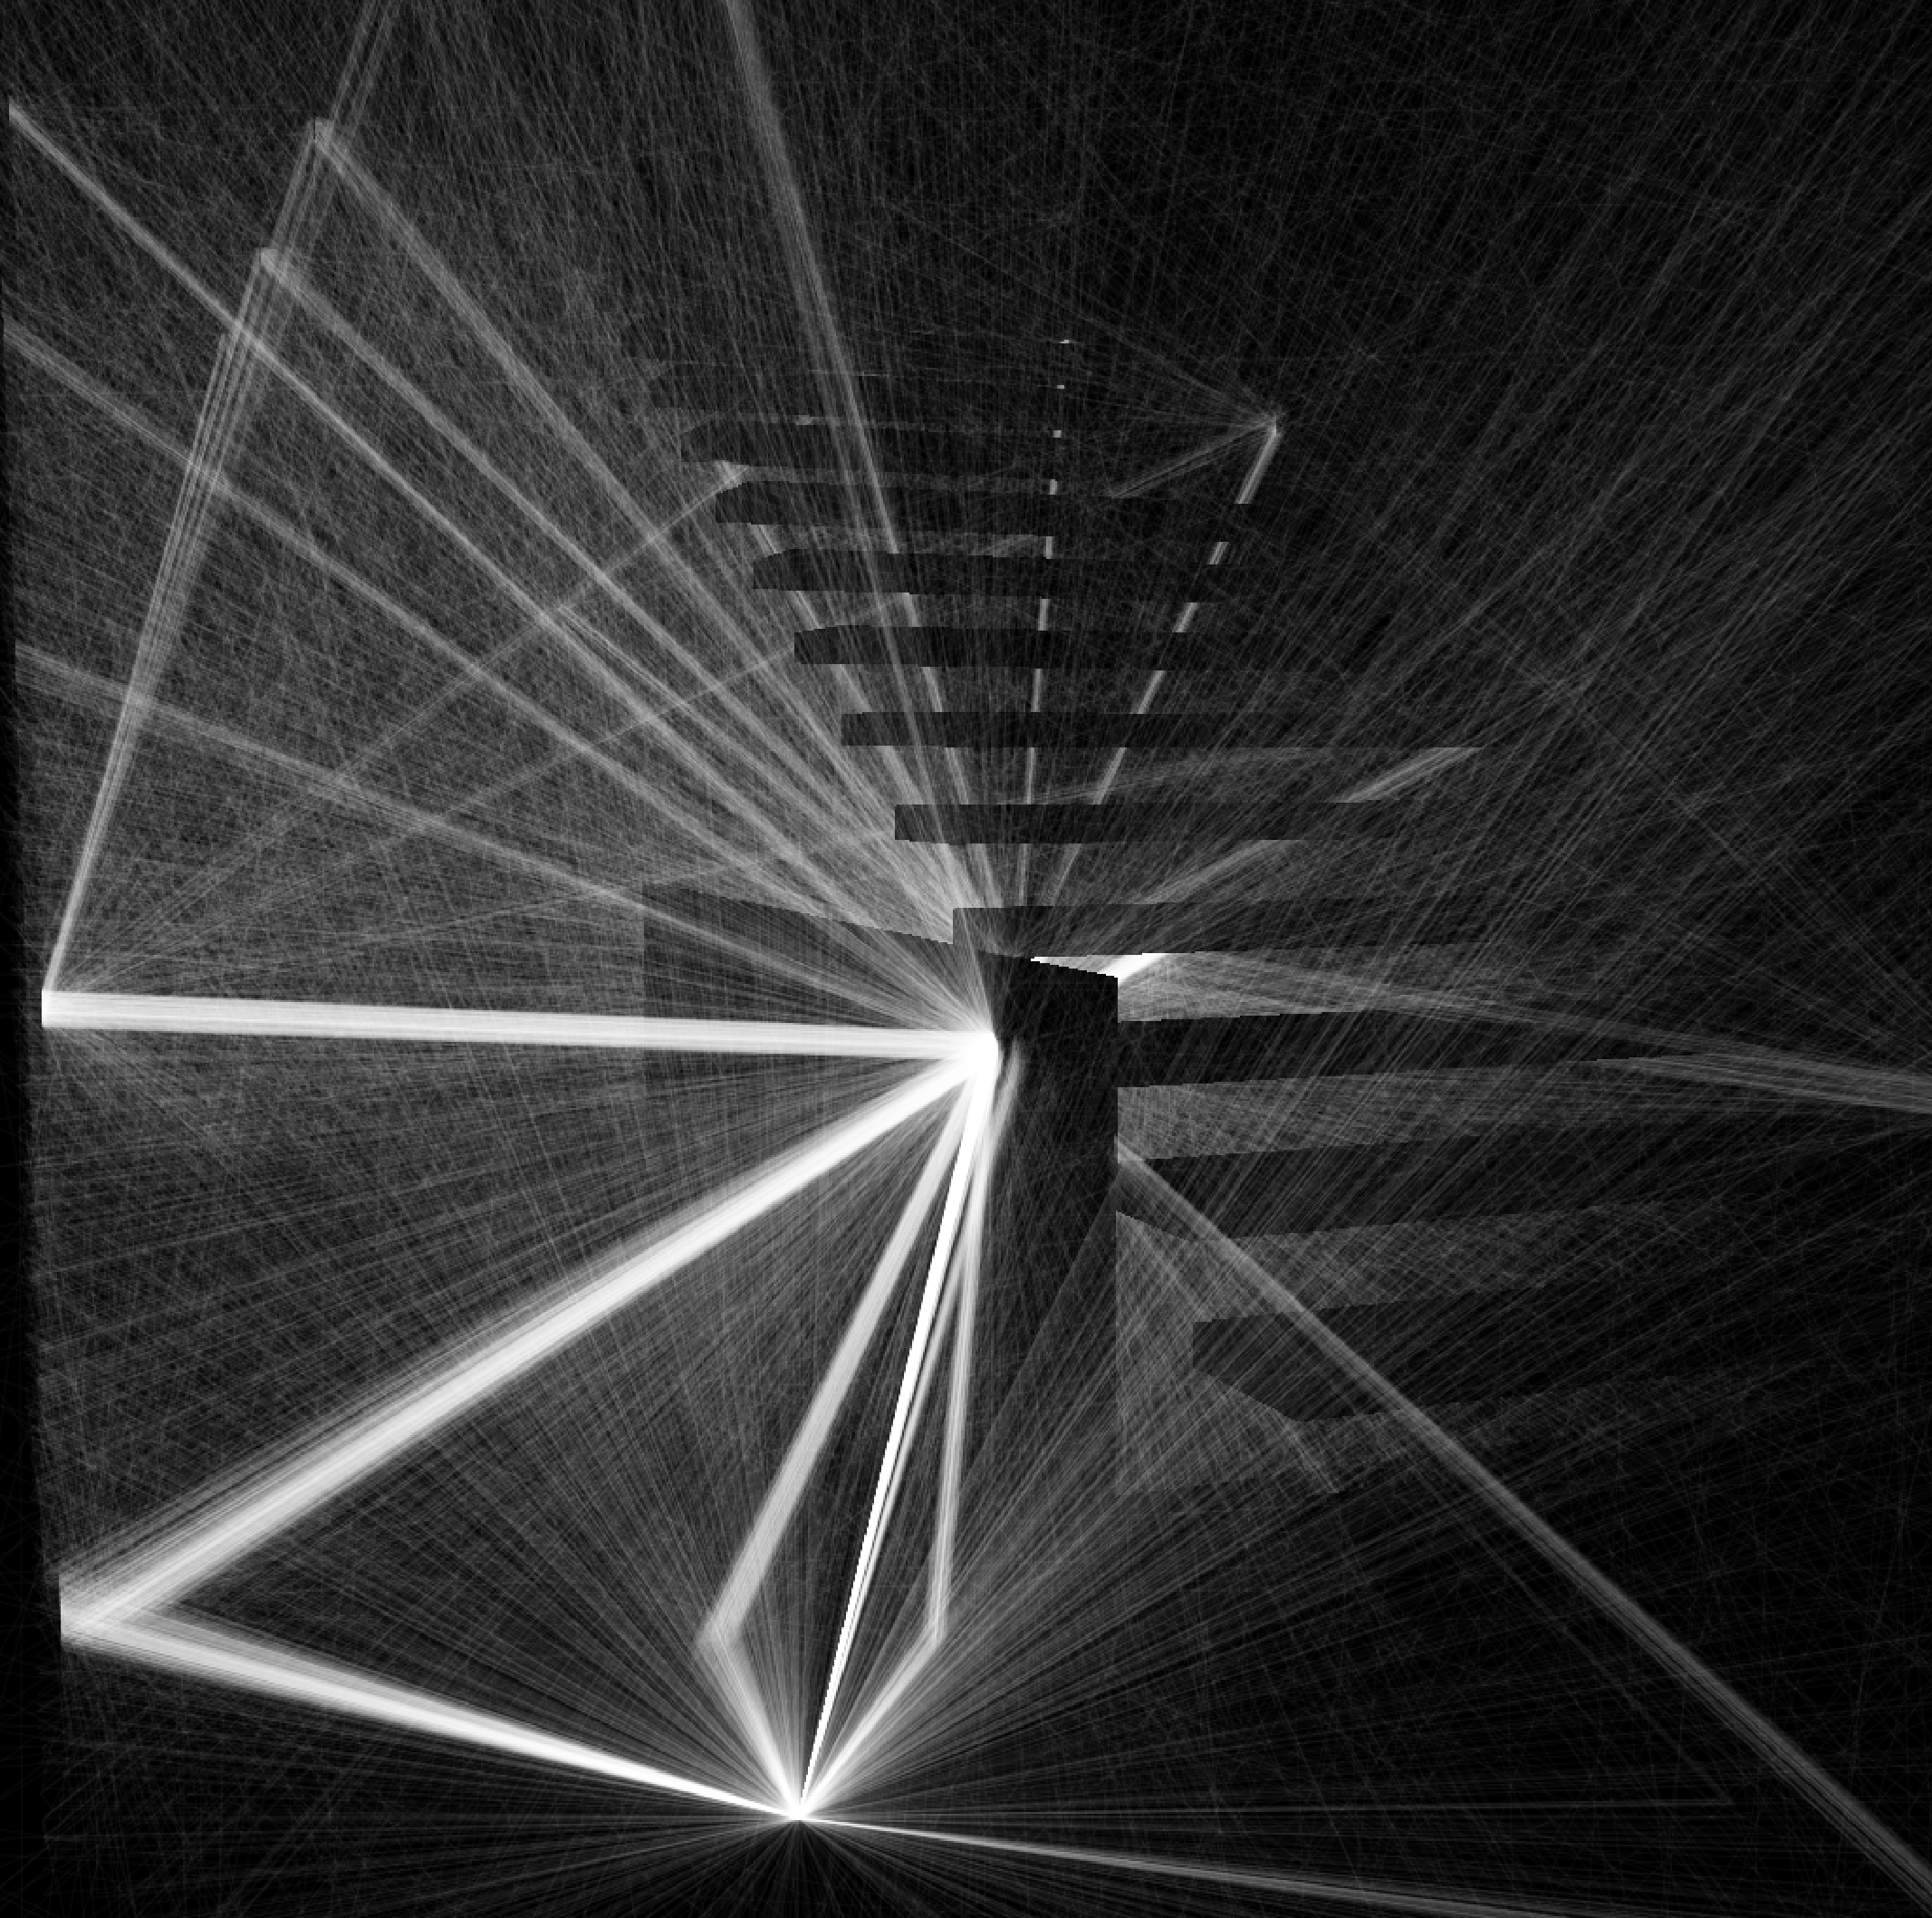
\includegraphics[width=\textwidth]{chapters/chapter_thetool/rays_front}
		\caption{\textit{Front} paths}
		\label{rays_front}
	\end{subfigure}
	\begin{subfigure}[t]{0.24\linewidth}
		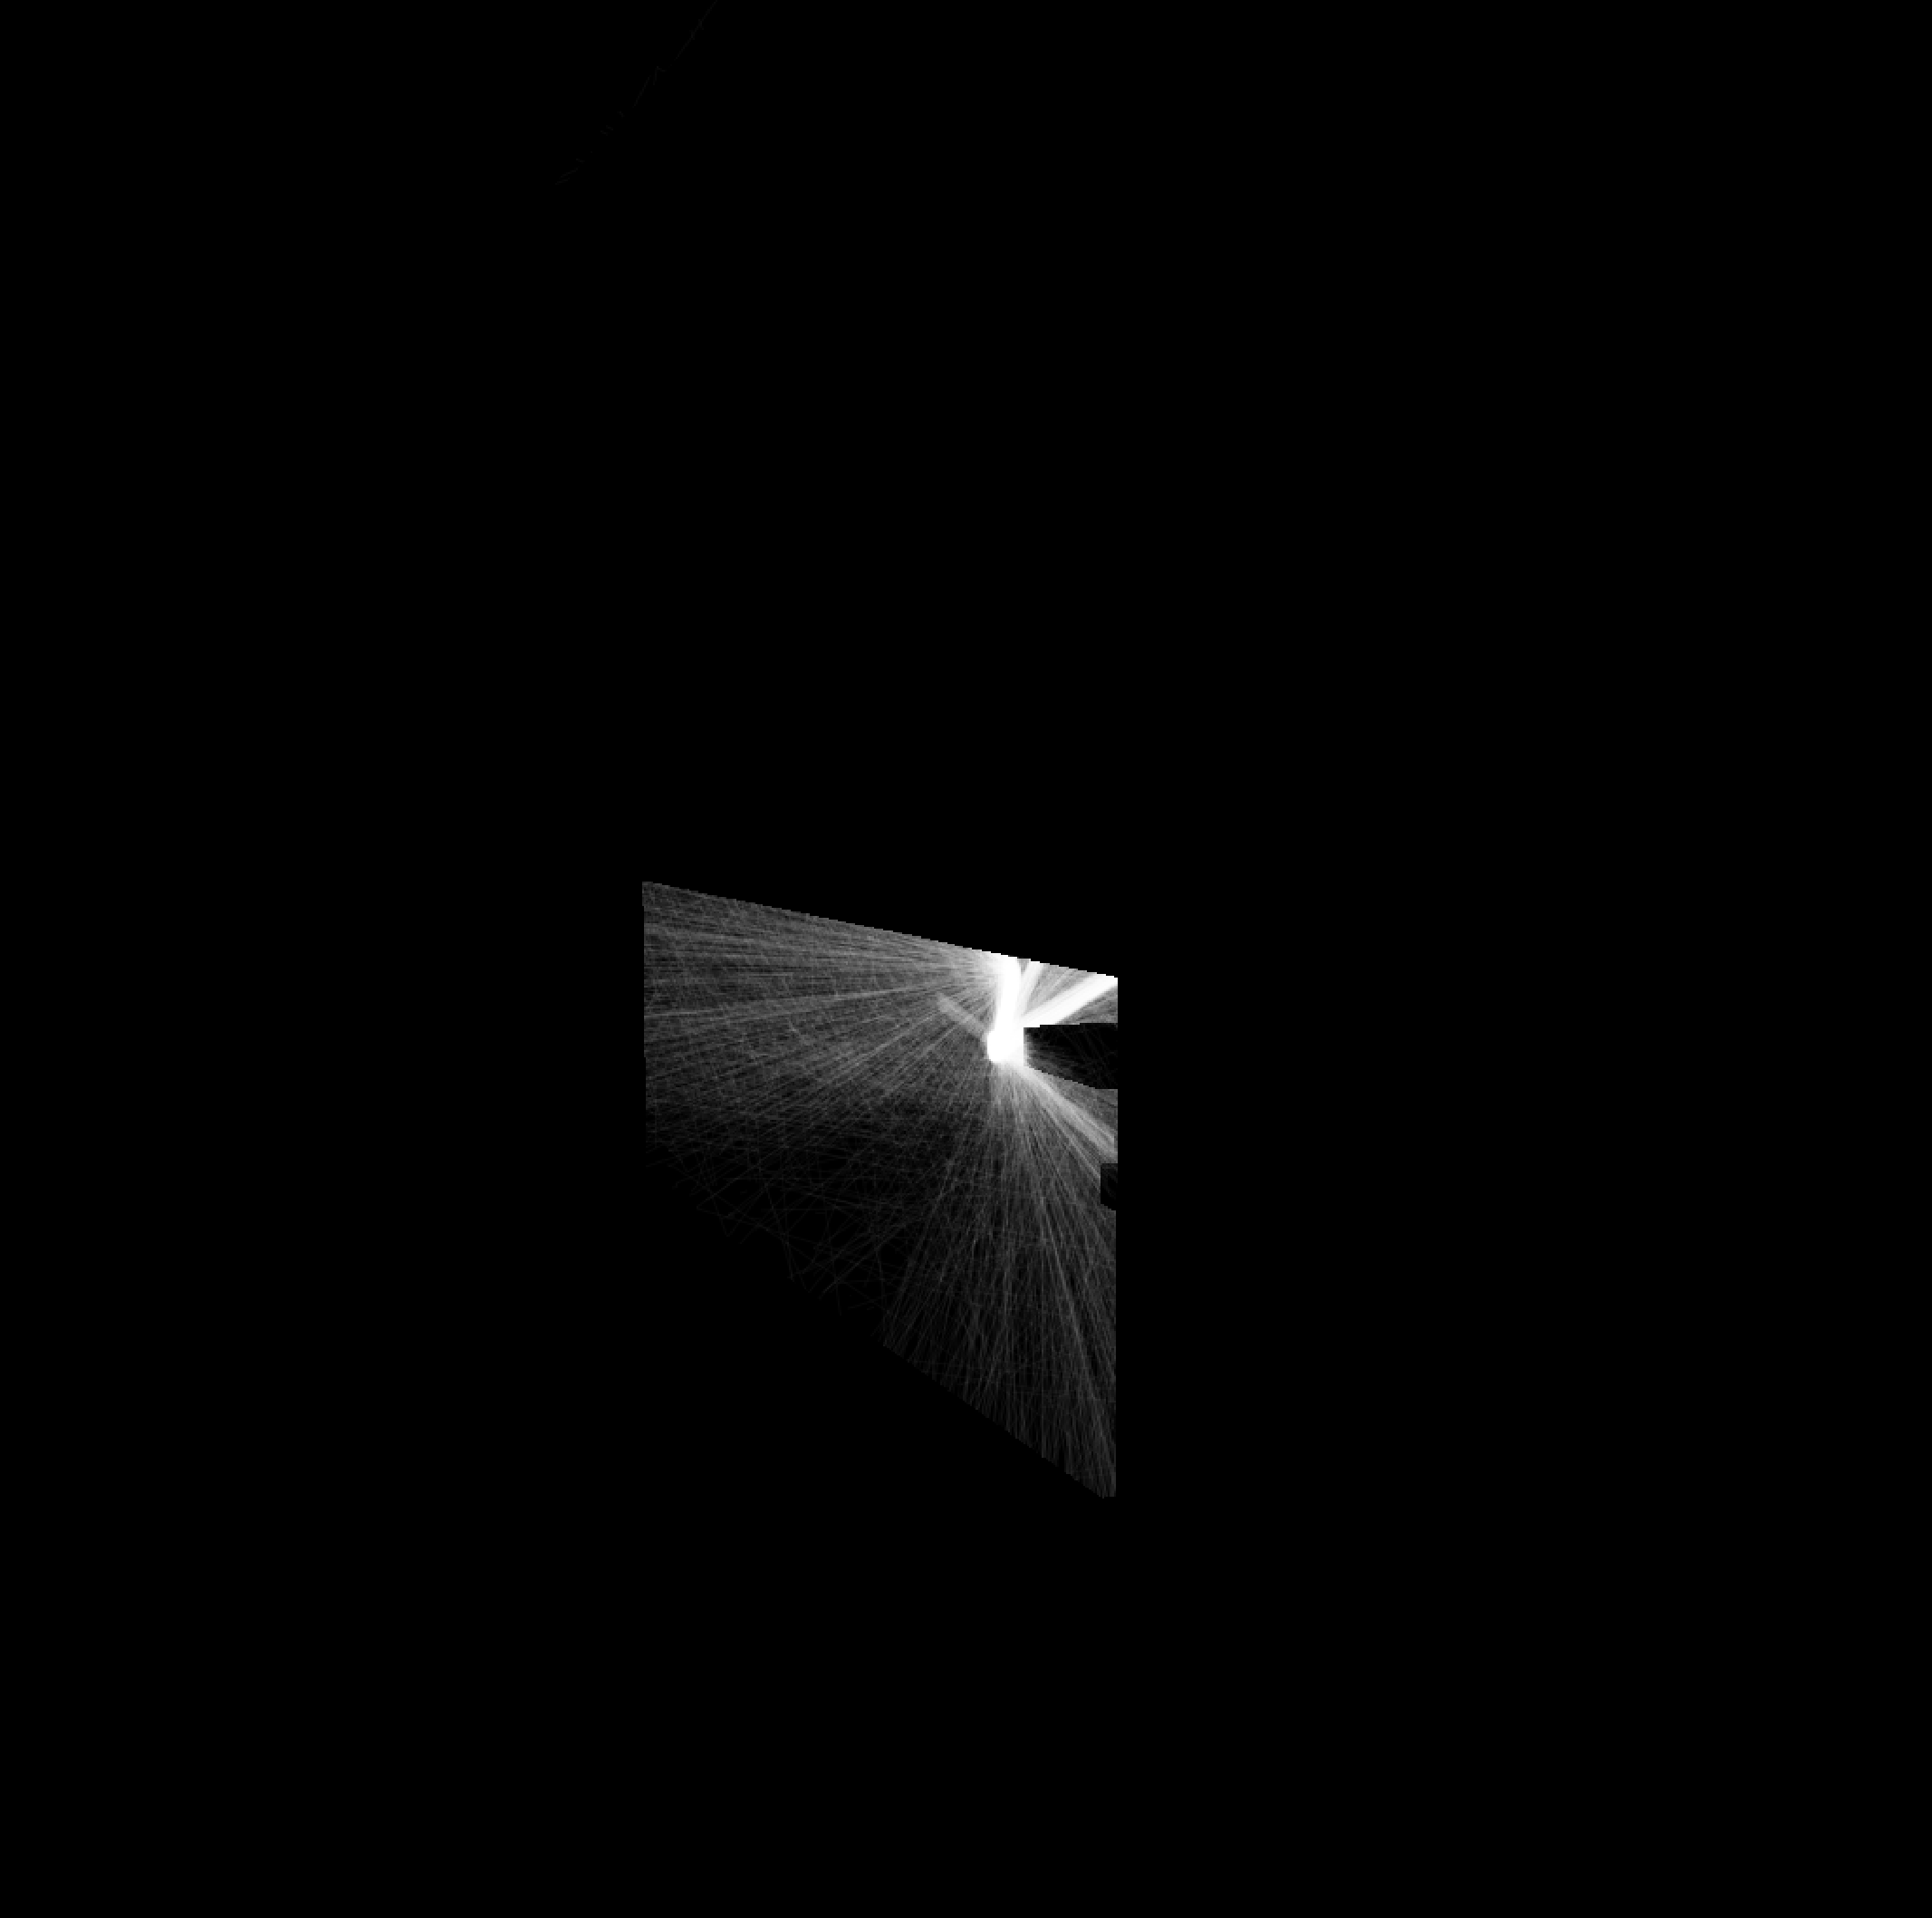
\includegraphics[width=\textwidth]{chapters/chapter_thetool/rays_back}
		\caption{\textit{Back} paths}
		\label{rays_back}
	\end{subfigure}
	\begin{subfigure}[t]{0.24\linewidth}
		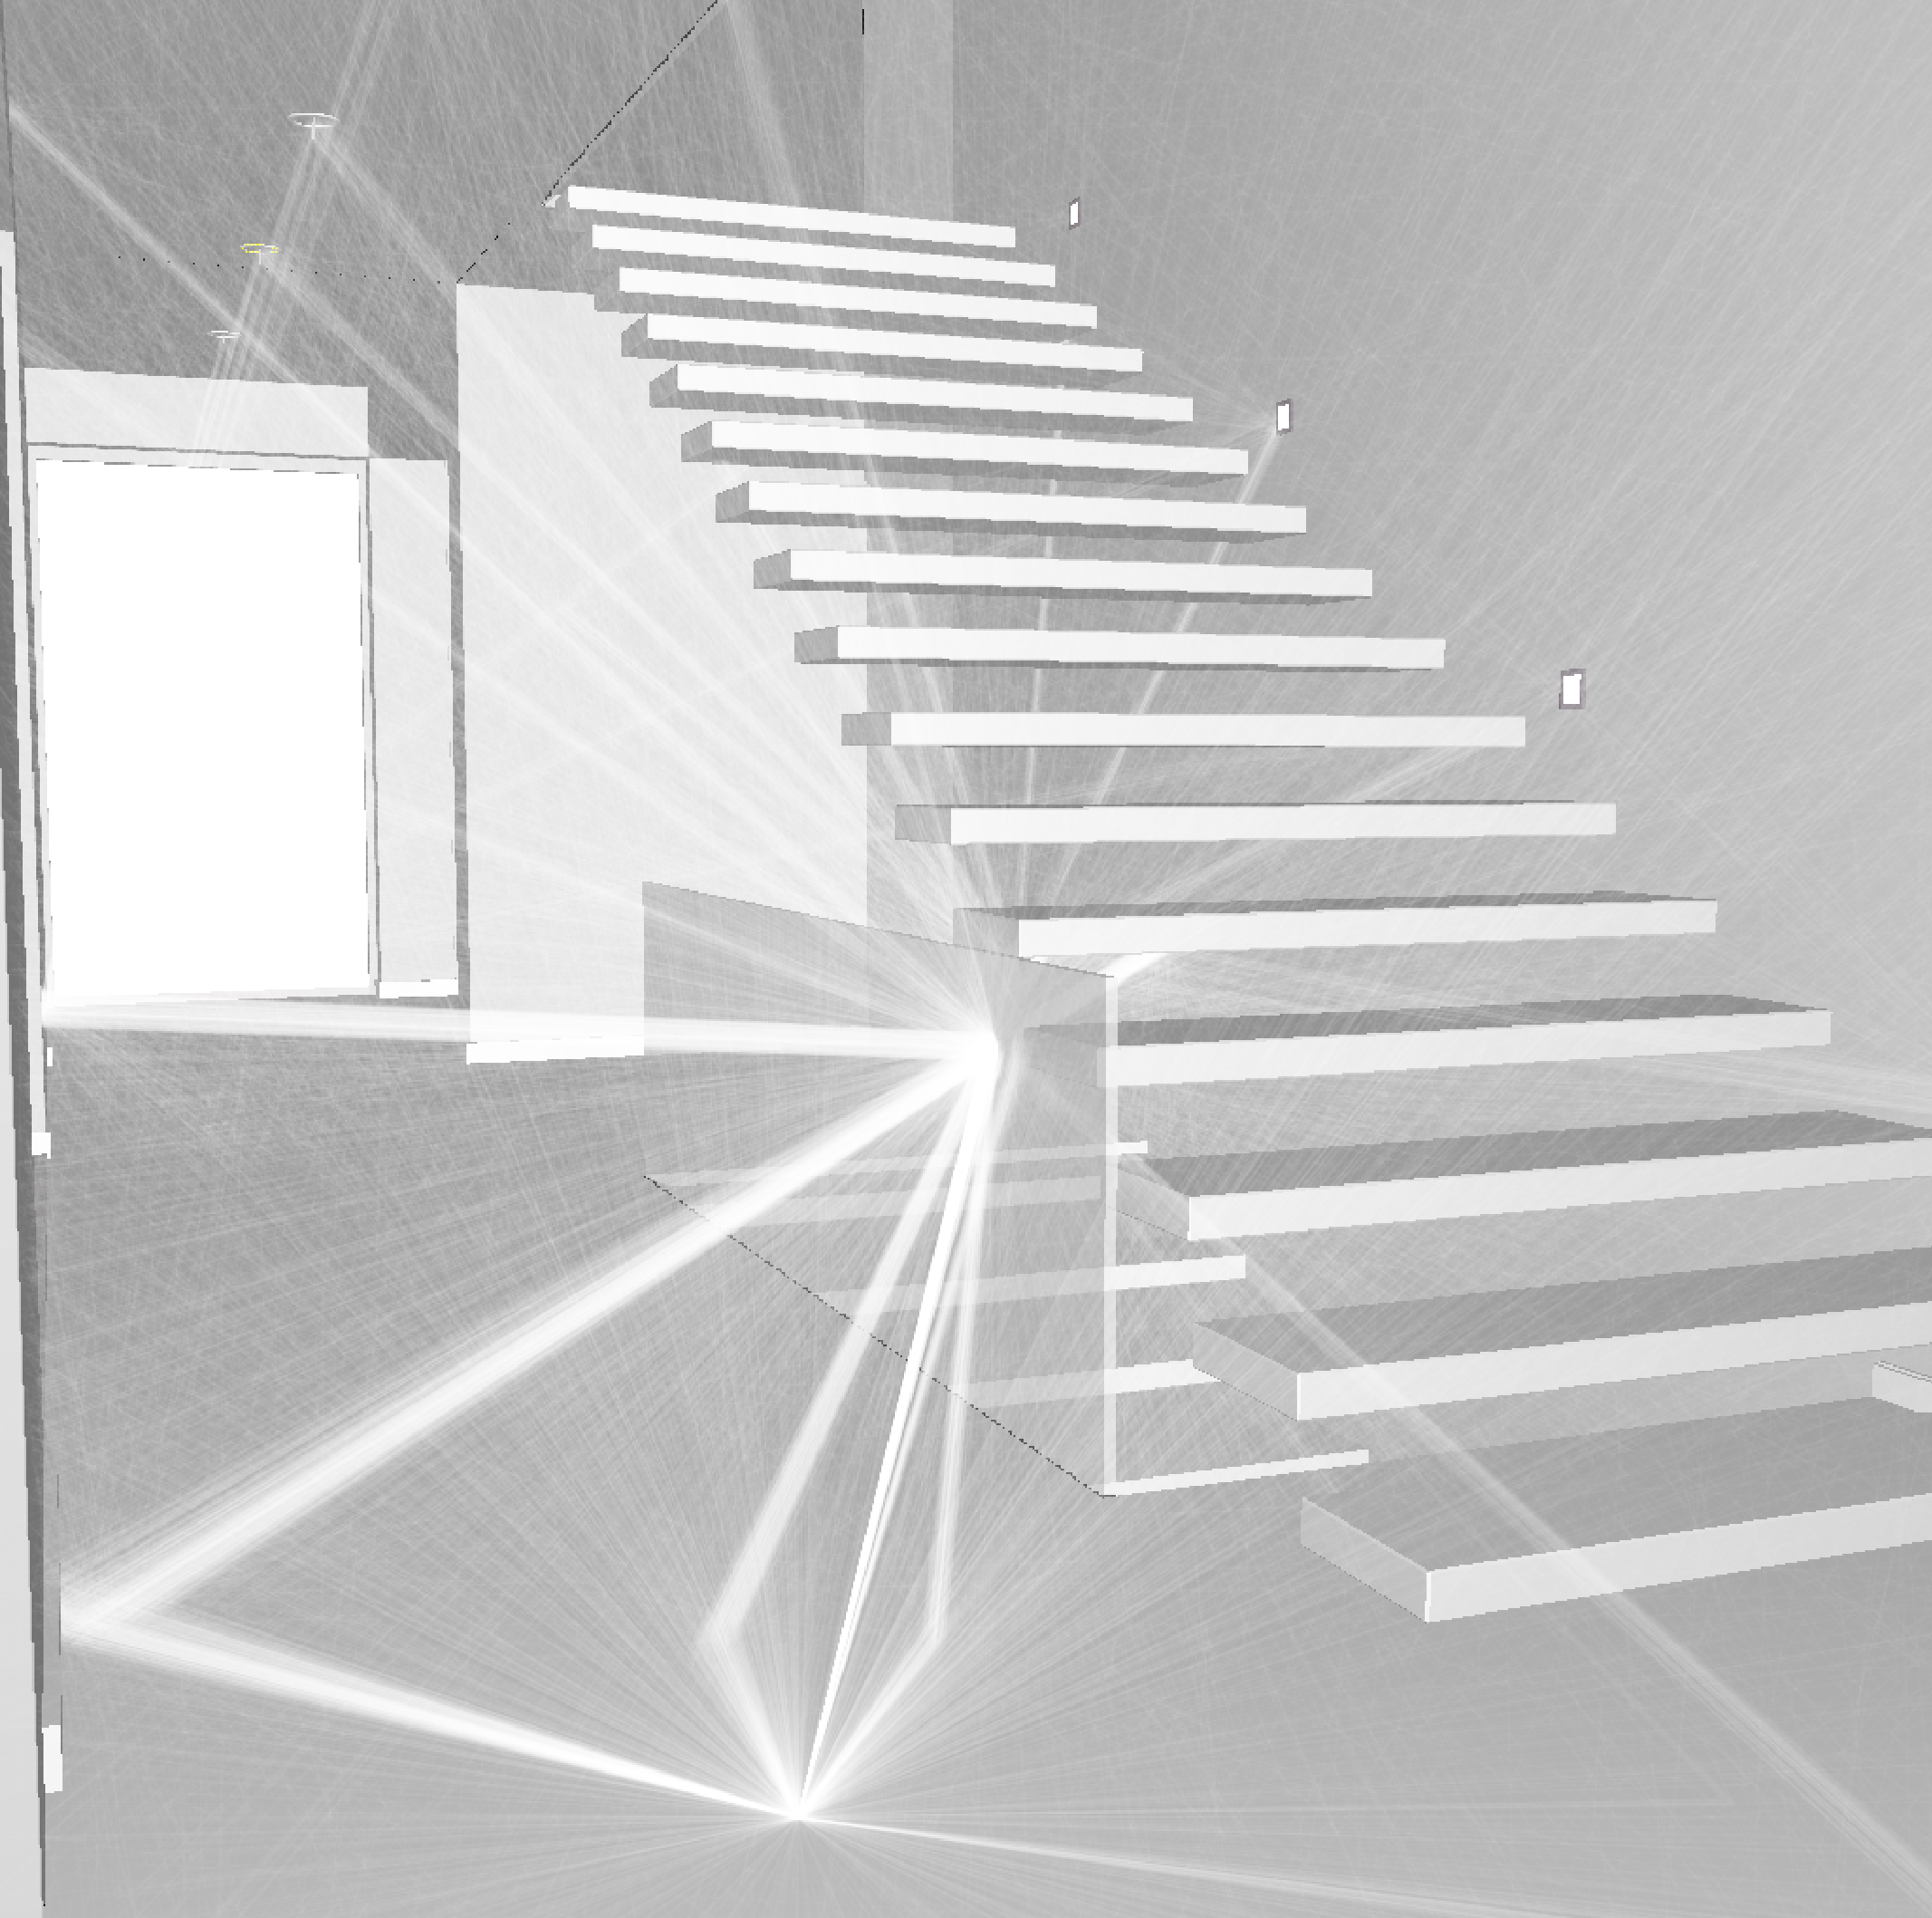
\includegraphics[width=\textwidth]{chapters/chapter_thetool/beauty+rays}
		\caption{Scene + paths}
		\label{beauty+rays}
	\end{subfigure}
	\begin{subfigure}[t]{0.24\linewidth}
		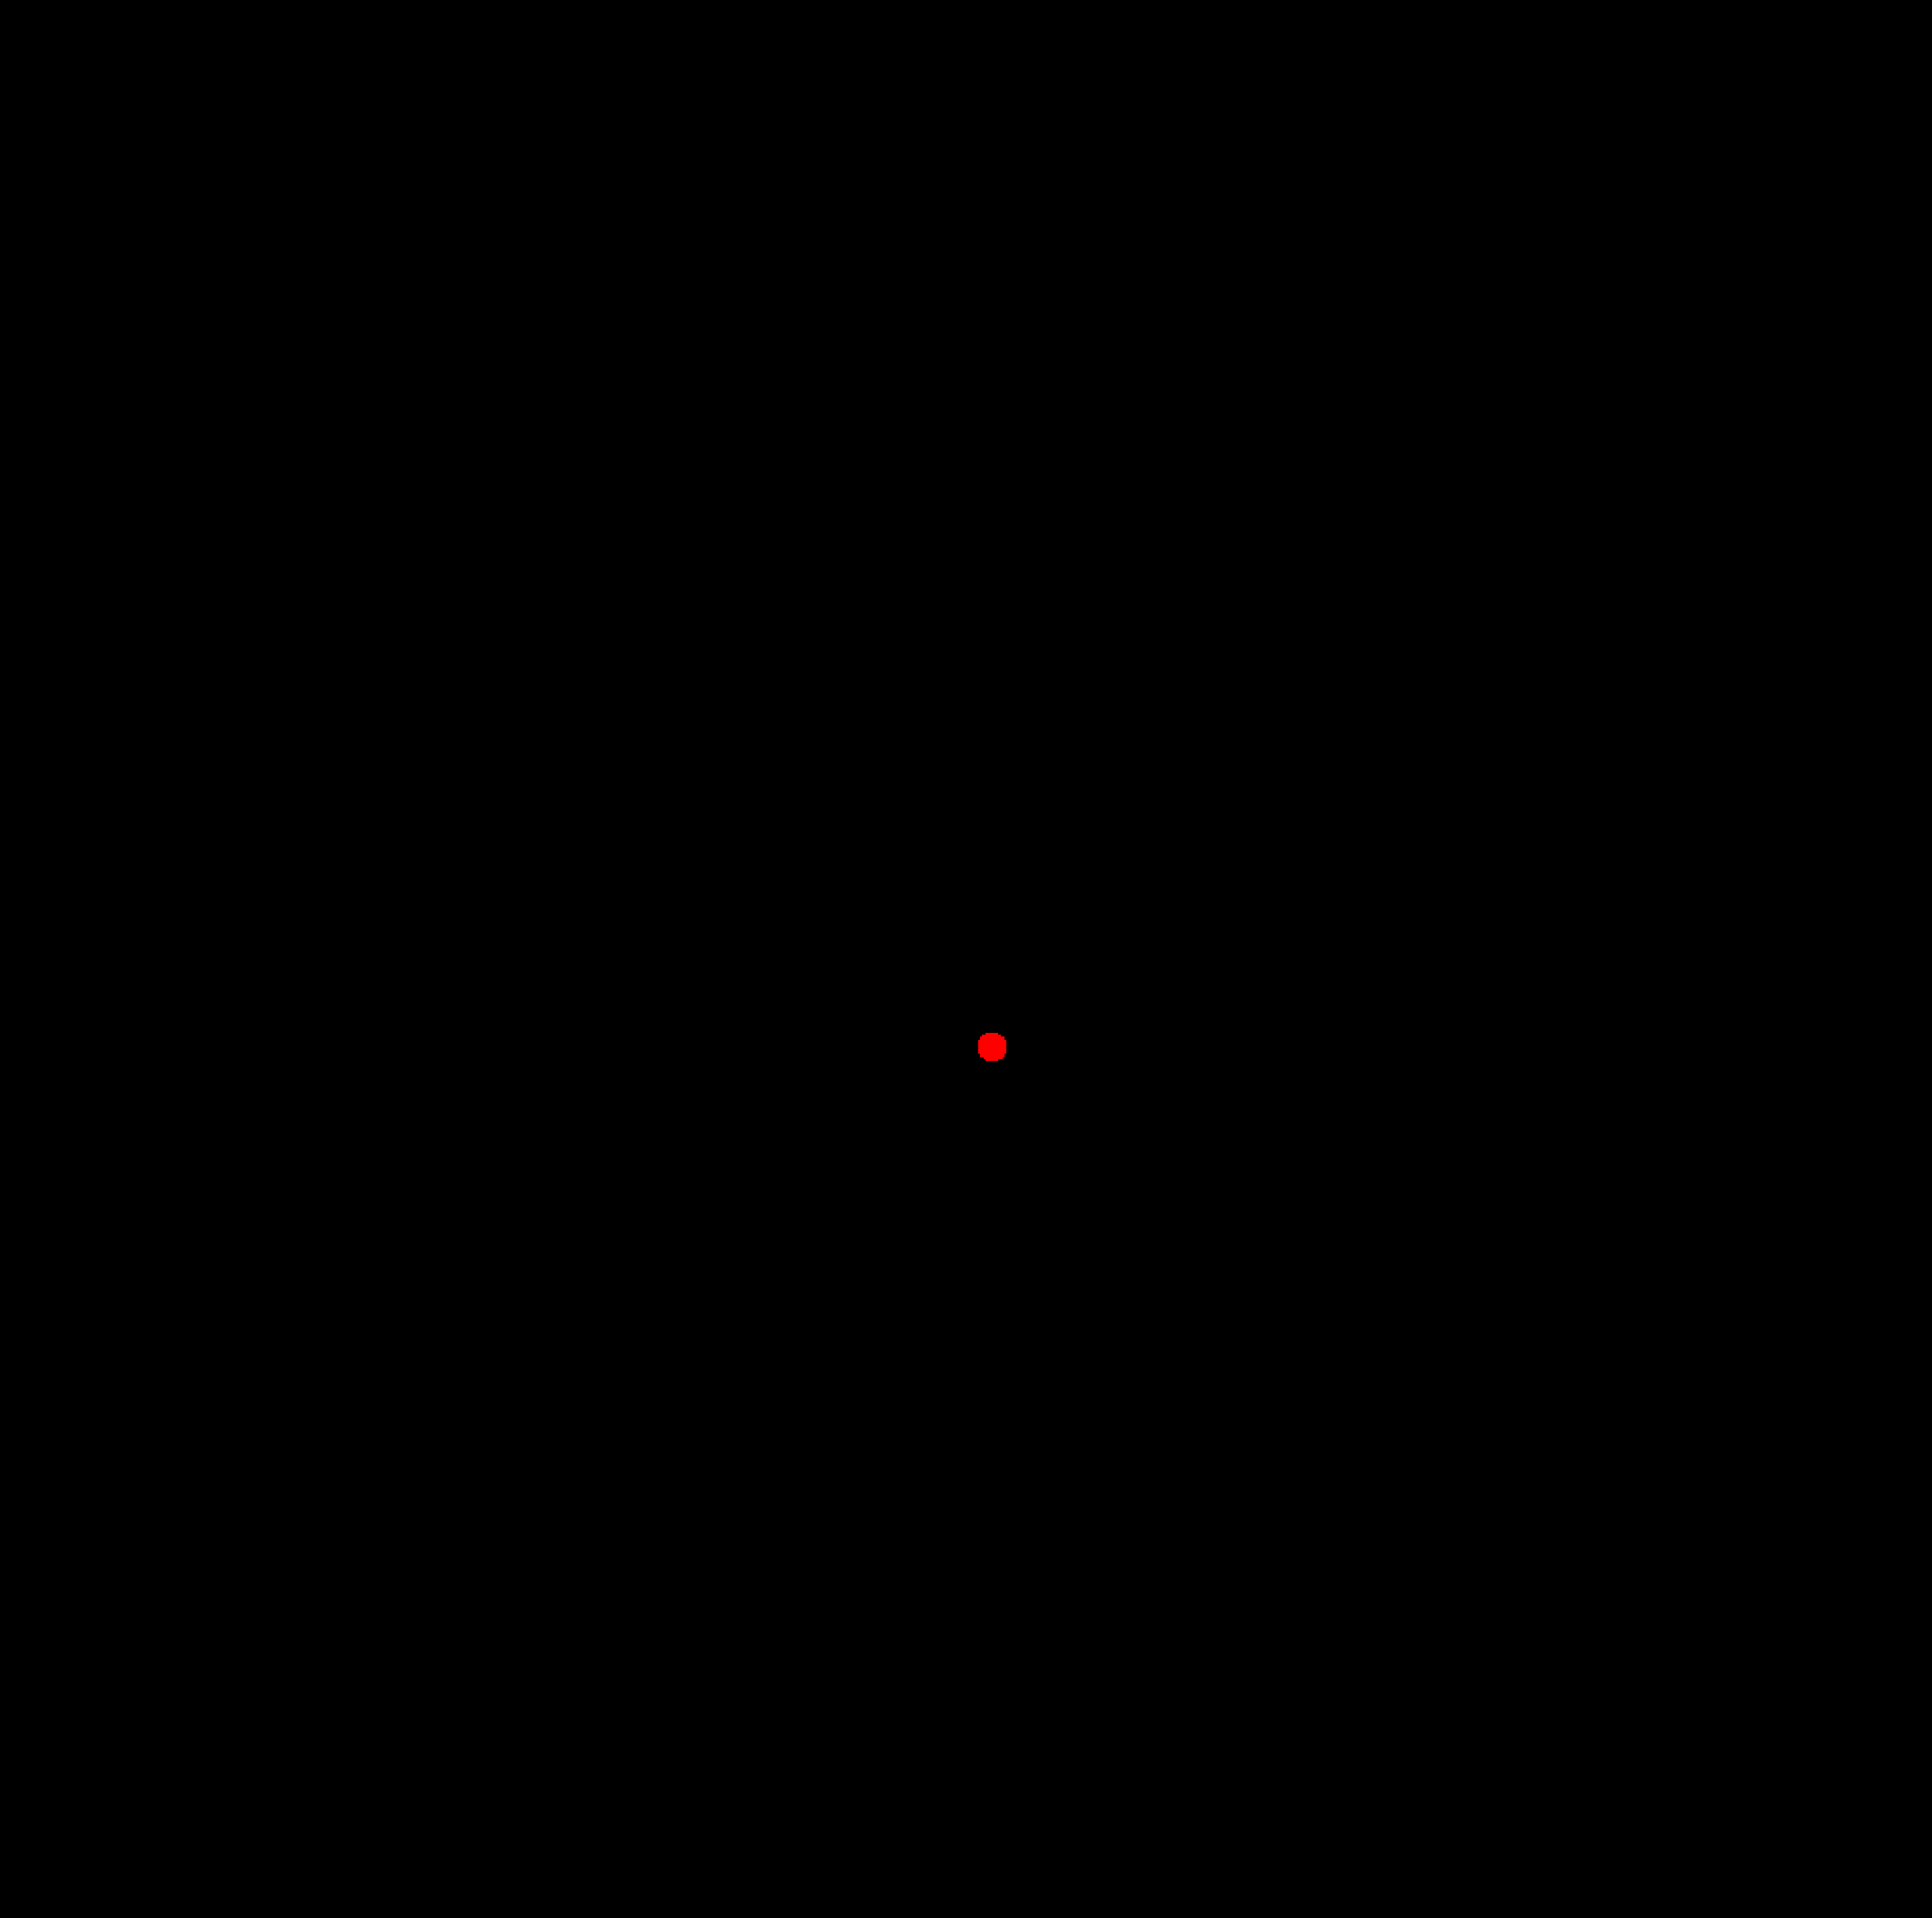
\includegraphics[width=\textwidth]{chapters/chapter_thetool/filter_mask}
		\caption{Filter mask}
		\label{filter_mask}
	\end{subfigure}

	\caption{Textures written by the paths pass with the composited result of the scene renders plus the paths and the filter mask texture.}
	\label{final_passes}
\end{figure}

%TODO think about a pipeline overview figure

\subsubsection{Camera controls}
Users can navigate the scene using camera controls common to many commercial animation suite packages:
\begin{description}
	\item[Alt key + Left mouse button drag] Tumbles the camera around a focus point in front of the camera.
	\item[Alt key + Right mouse button drag] Dollies the camera.
	\item[Alt key + Middle mouse button drag] Tracks the camera. 
\end{description}
At this moment, camera controls are rather coarse and could use some polishing; for example, their sensitivity does not adapt to changes in scene size and this leads to difficulties while navigating small or big scenes. Even the clipping planes ignore the scene size and the default values often create artifacts. Still taking inspiration from commercial packages, camera controls can also be combined with the mechanic of selecting geometries from the viewport to make the camera orbit around a geometry on a key press.

\subsubsection{Axes widget}

Imitating most 3d applications, a small floating panel showing the current camera orientation by a render of the three coordinate axes is provided. The x-axis is colored in red, the y-axis in green, and the z-axis in blue, following the well established convention in computer graphics. The rendering of it is done without any vertex buffer since the vertices are positioned by the vertex shader using the \texttt{gl\_VertexID} built-in GLSL variable and some bit-wise operations. 

\subsection{Render image widget}
\label{image_widget}

\begin{figure}
	\centering
	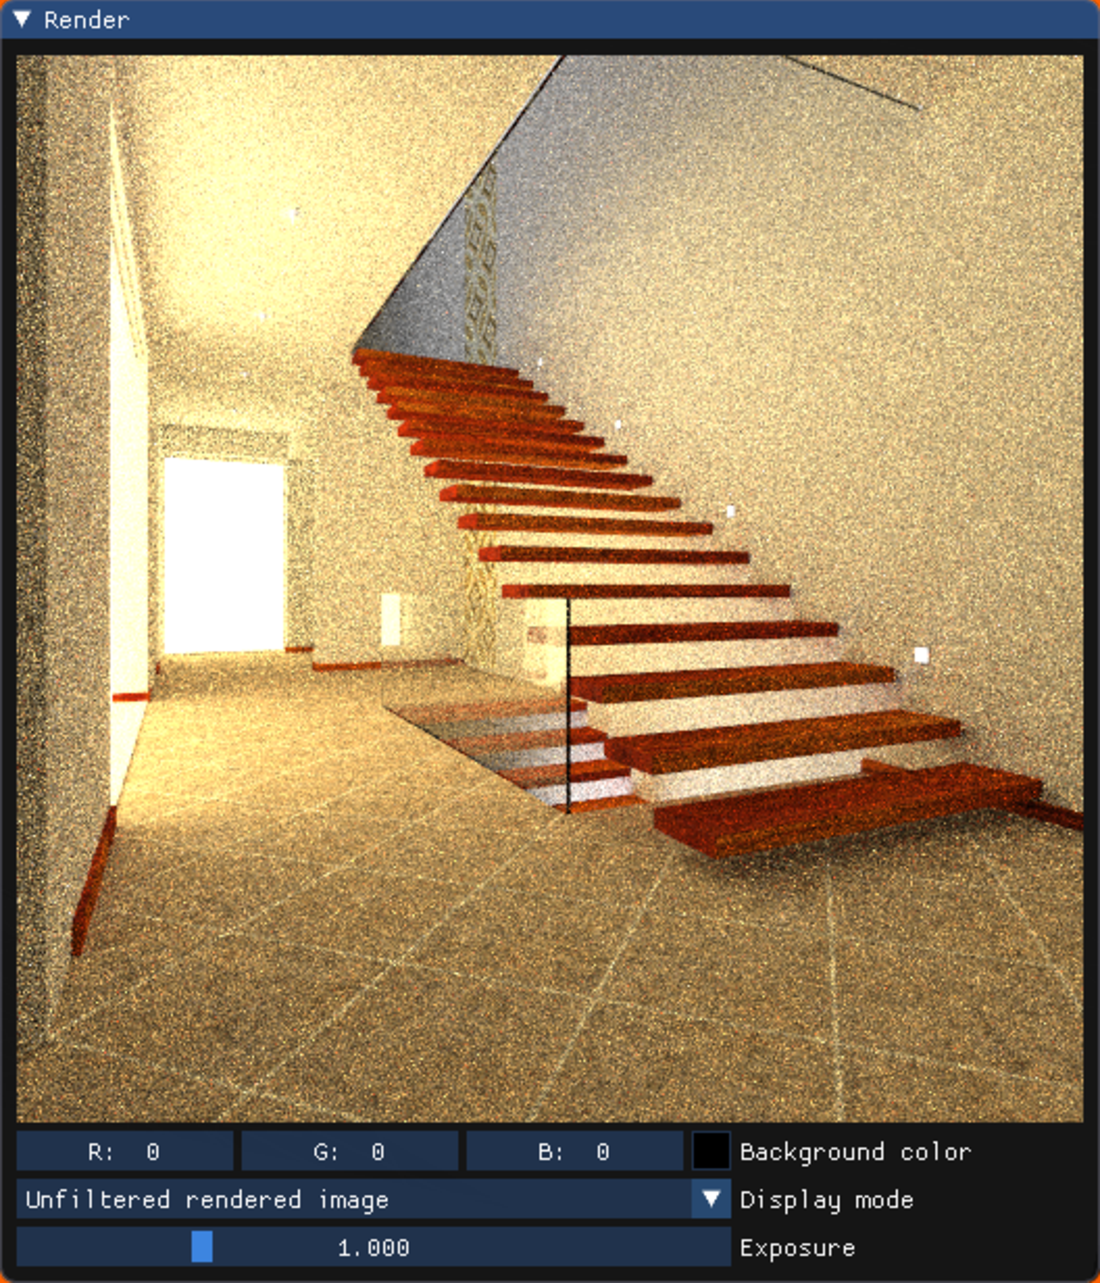
\includegraphics[width=0.5\textwidth]{chapters/chapter_thetool/imagewidget_full}
	\caption{\textbf{“Render”} panel in its default state, showing an unaltered render of the \textit{Modern Hall} \cite{bitterliscenes} scene.}
	\label{imagewidget_full}
\end{figure}

\begin{figure}
	\centering
	\begin{subfigure}[t]{0.32\linewidth}
		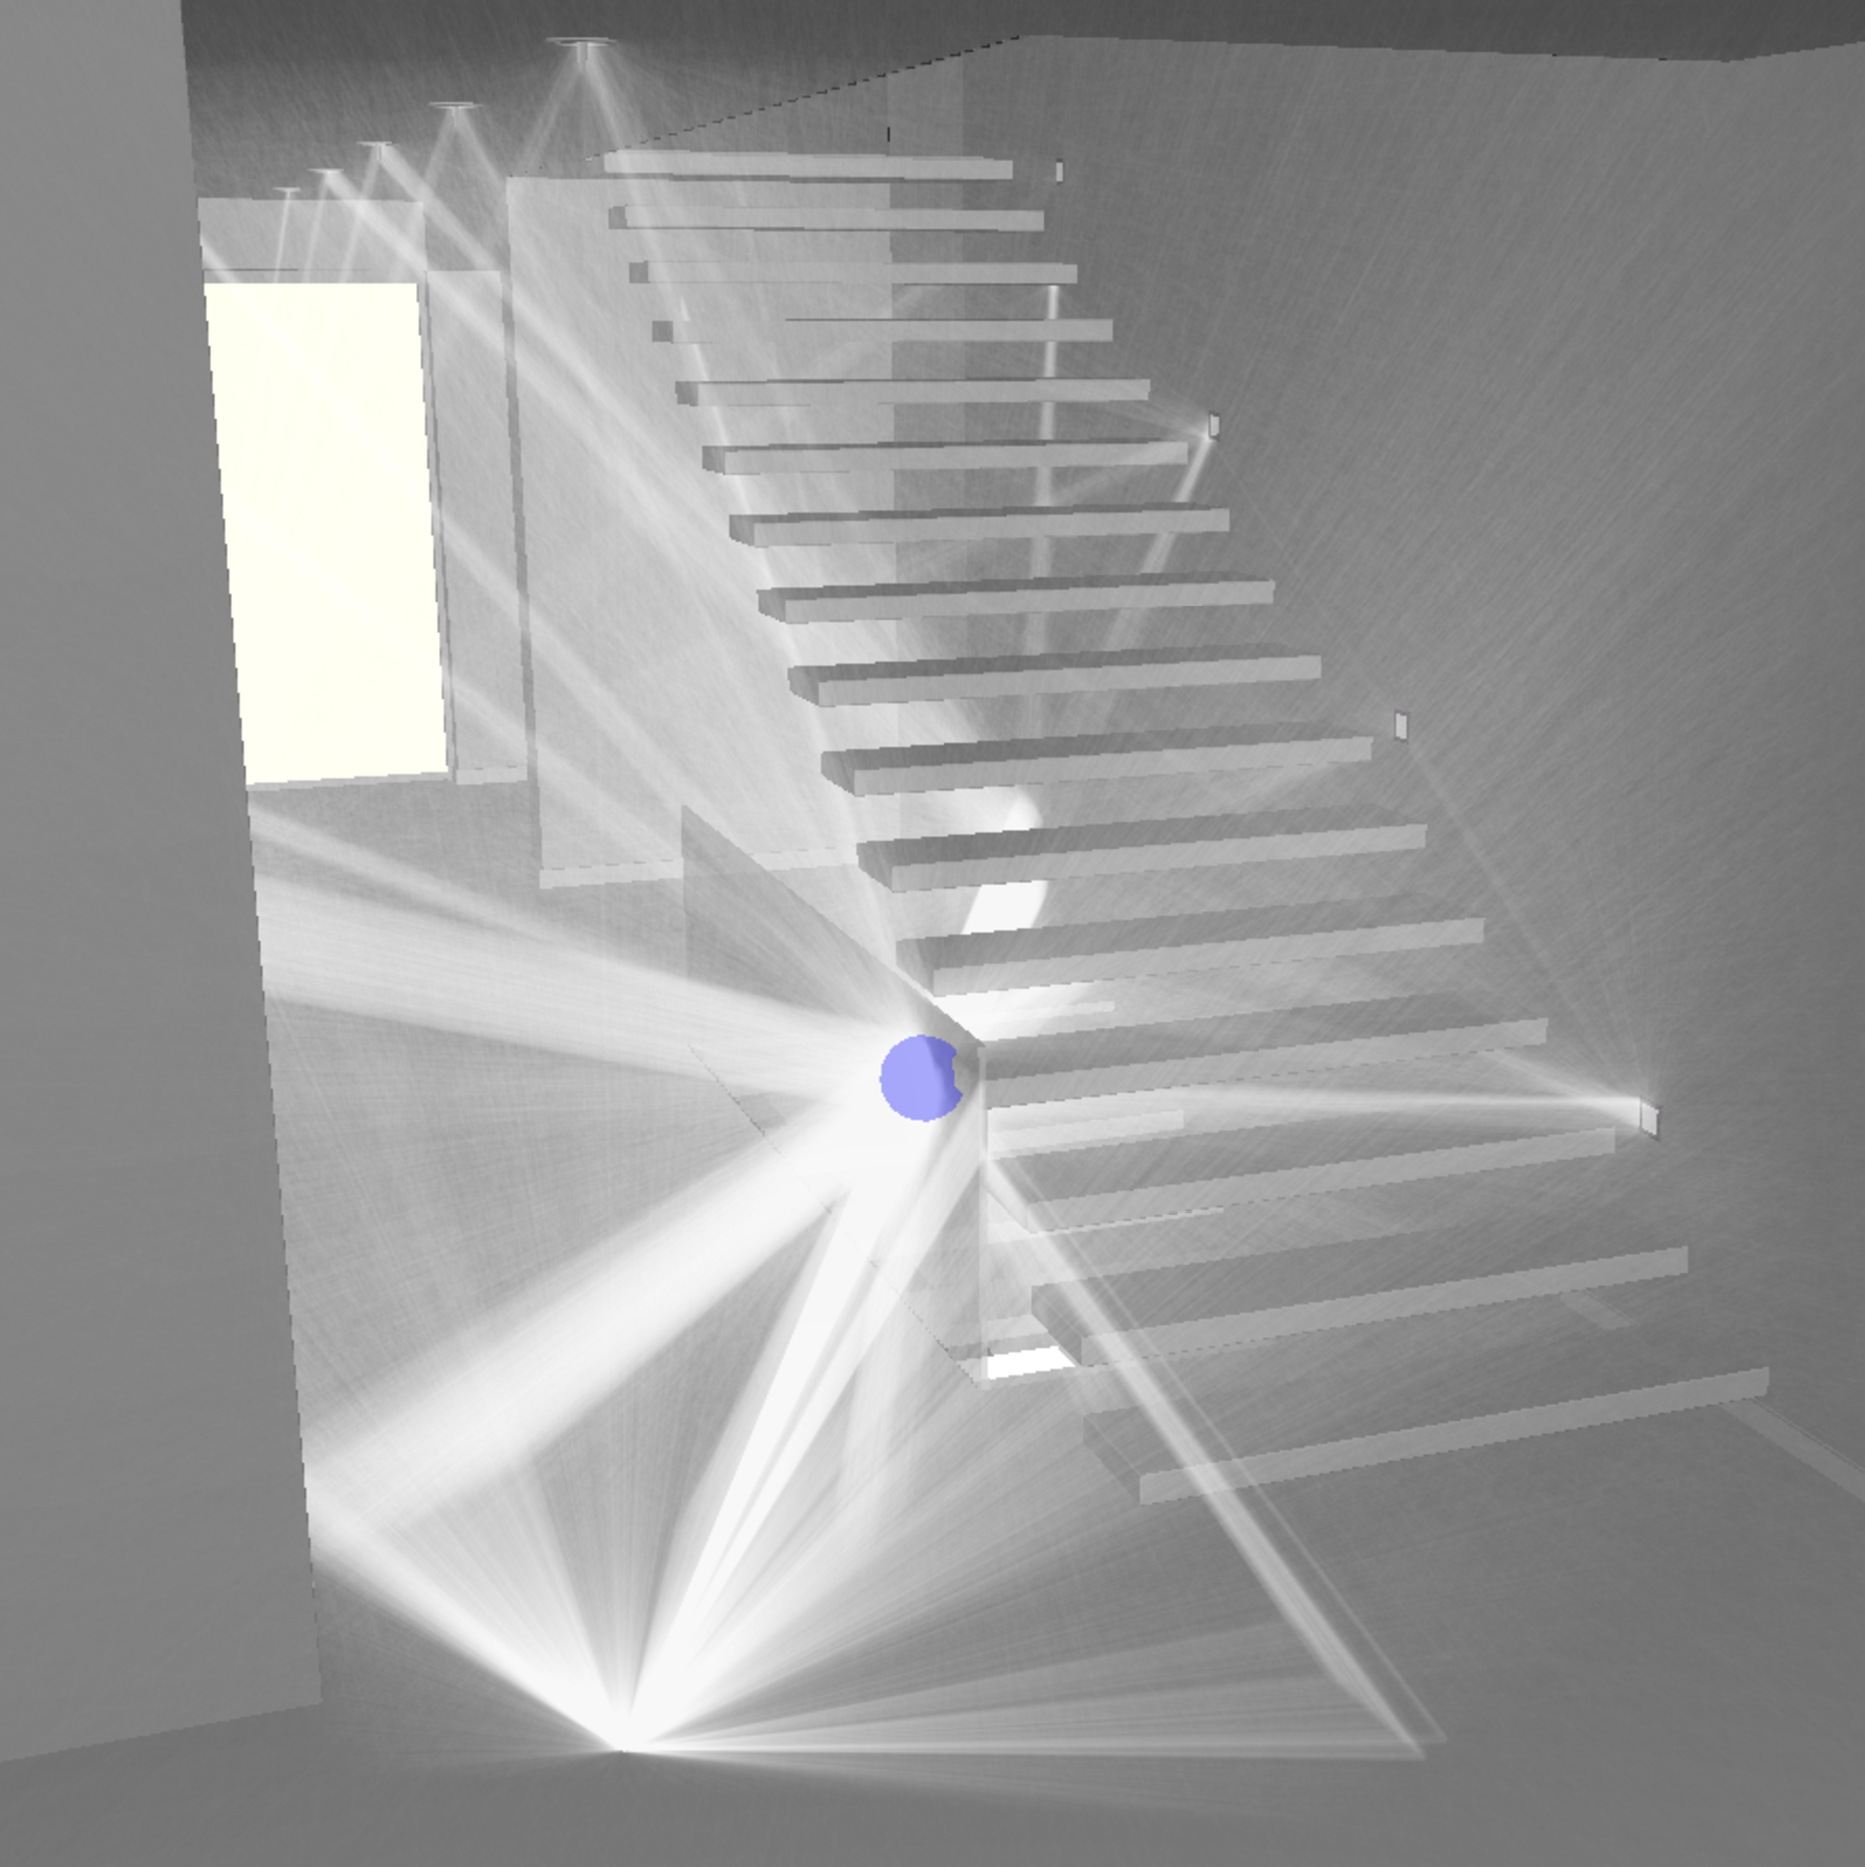
\includegraphics[width=\textwidth]{chapters/chapter_thetool/imagewidget_paths}
		\caption{Viewport render}
		\label{imagewidget_paths}
	\end{subfigure}
	\begin{subfigure}[t]{0.32\linewidth}
		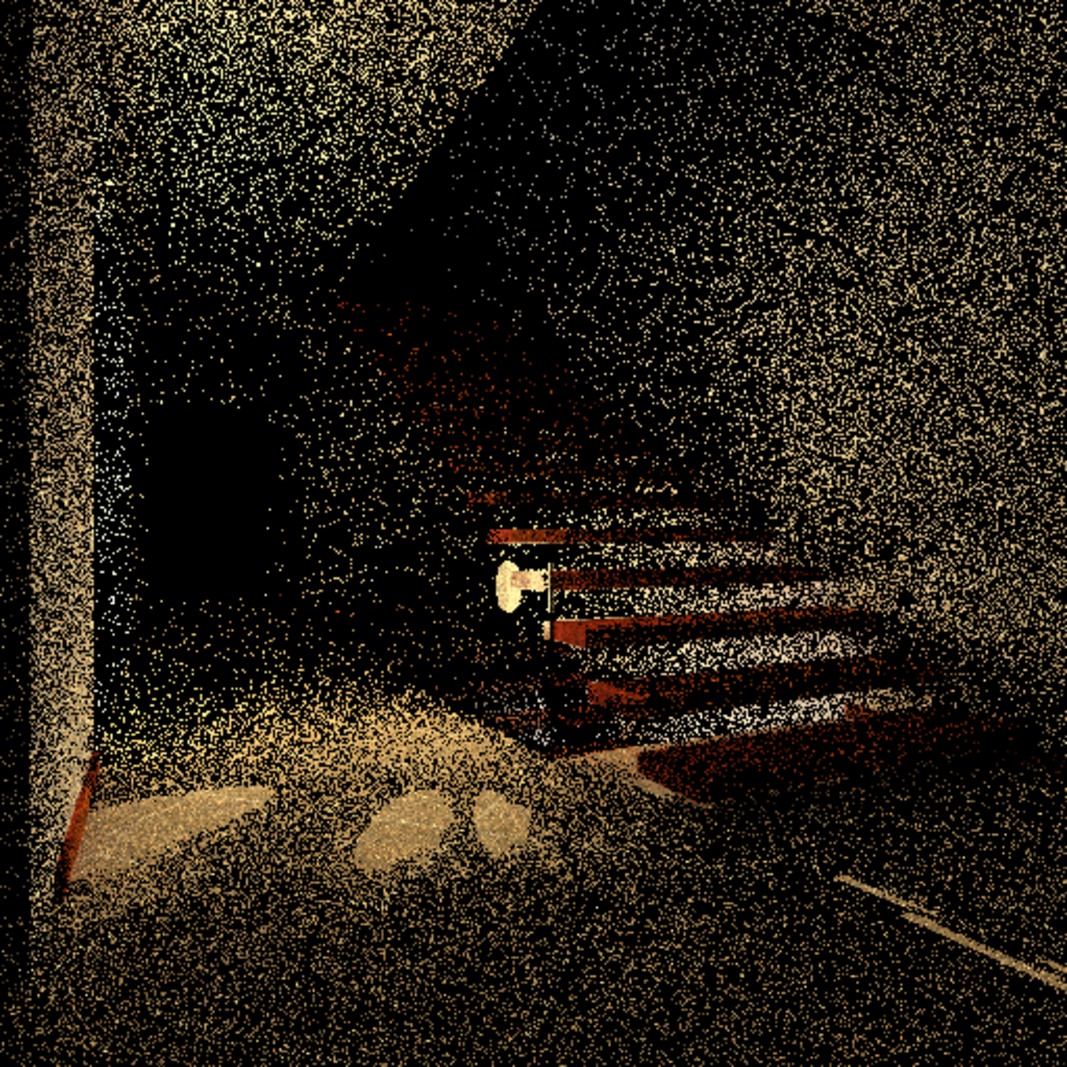
\includegraphics[width=\textwidth]{chapters/chapter_thetool/imagewidget_radiance}
		\caption{Radiance view}
		\label{imagewidget_radiance}
	\end{subfigure}
	\begin{subfigure}[t]{0.32\linewidth}
		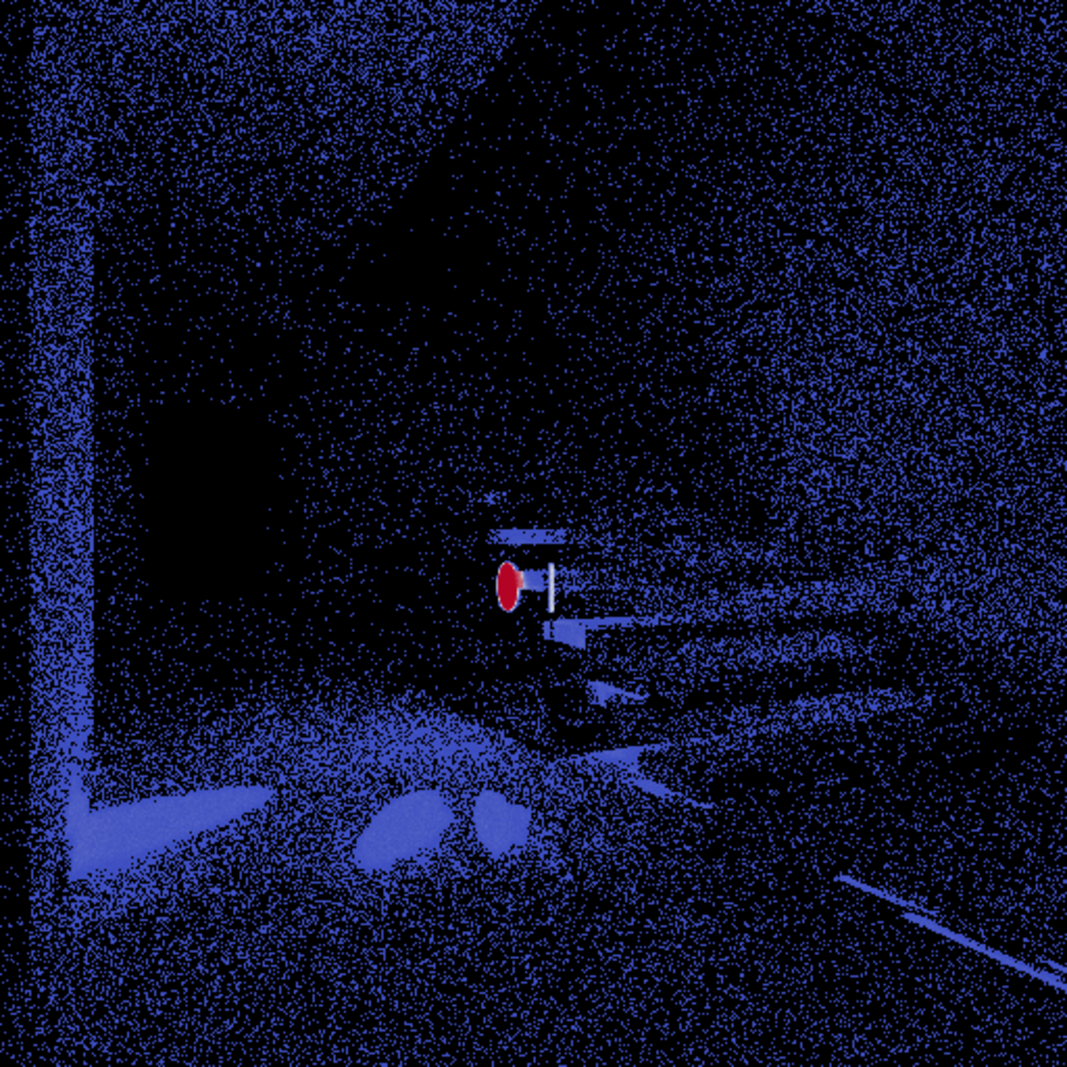
\includegraphics[width=\textwidth]{chapters/chapter_thetool/imagewidget_bounces}
		\caption{Bounces view}
		\label{imagewidget_bounces}
	\end{subfigure}

	\caption{An example of the \textbf{“Final radiance”} (b) and \textbf{“Paths per pixel”} (c) views of the \textbf{“Render”} panel relative to the selected paths shown in a viewport capture (a).}
	\label{imagewidget_options}
\end{figure}


The render image is a vital part of a dataset, after all it is the end result of a path tracer. A panel, simply called \textbf{“Render”}, is dedicated to showing the render image and some useful views related to it. By default, as soon as a dataset is loaded from disk, a pristine render image built upon the radiance and camera samples buffers of the dataset\footnote{Refer to section \ref{datatogather} for information about the buffers of the dataset} (fig. \ref{imagewidget_full}). Due to its nature, this image has a high dynamic range and it has a linear color space, so a tone mapping operation has been applied on it through a fragment shader. The tone mapping described on the OpenEXR documentation\footnote{\url{https://www.openexr.com/using.html}} is used here and its \textit{exposure} parameter has been directly linked to the \textbf{“Exposure”} slider; users can tweak it to explore the dynamic range of the render.

When some path filters have been placed into the scene, users can access the \textbf{“Final radiance”} and the \textbf{“Paths per pixel”} views using the \textbf{“Display mode”} drop-down list. They both show information about the pixels affected by the currently selected paths and the pixels not touched by the path selection are rendered of the color specified by the user through the \textbf{“Background color”} color picker. The \textbf{“Final radiance”} view (fig. \ref{imagewidget_radiance}) simply displays the pixels of the final image; it was thought of actually displaying the radiance carried only by the selected paths, but as per today it is still to implement. The \textbf{“Paths per pixel”} view (fig. \ref{imagewidget_bounces}) instead shows for each pixel the number of paths originated on it, fitted to $[0,1]$ using the maximum and minimum as extremes and then color mapped with the \textit{coolwarm} scheme\footnote{The \textit{coolwarm} scheme is a $\mathbb{R} \to \mathbb{R}^3$ mapping that maps a scalar $\in[0,1]$ to an RGB color. $0$ gets mapped to $(0.230, 0.299, 0.754)^\intercal$, $0.5$ to $(0.865, 0.865, 0.865)^\intercal$, $1$ to $(0.706, 0.016, 0.150)^\intercal$, and all scalars in between are linearly interpolated.}. In other words, it shows the density of paths for each pixel.

The only controls the user has on this widget are the already mentioned \textbf{“Exposure”} slider and the \textbf{“Background color”} color picker. As a future development, panning and zooming controls for the image plus some other controls on the tone mapping have been proposed.

\subsection{Bounce density heatmap}
\label{heatmap}

\begin{figure}
	\centering
	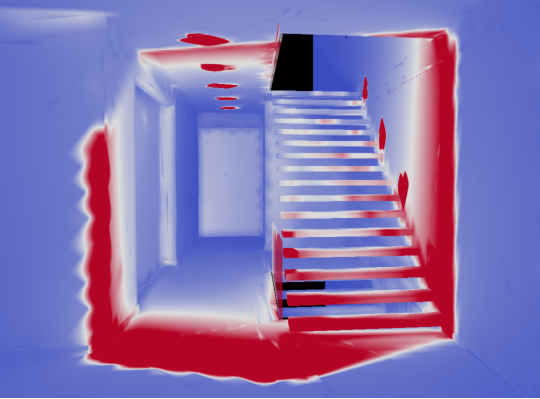
\includegraphics[width=0.6\textwidth]{chapters/chapter_thetool/heatmap}
	\caption{Viewport render of the \textit{Modern Hall} \cite{bitterliscenes} scene with the bounce density heatmap relative to a dataset generated by Yocto/GL \cite{pellacini2019yocto} on top of it.}
	\label{heatmap}
\end{figure}

In some cases, especially when exploring datasets generated upon scenes the user is not familiar with, it is difficult to place filters in a meaningful way. To be able to do that, approximate insight on how all the paths interact with the scene is needed. Up to what has been described until now, the only way in the tool to render paths by actually rasterizing their rays over a scene render; this, as already mentioned before and shown in figure \ref{visual_clutter}, gets quickly unmanageable and rather useless due to heavy visual cluttering.
This is where the \textit{bounce density heatmap} enters the game. As its name partially suggests, it is a heatmap that shows the density of path bounces on the surfaces of the scene. As shown in figure \ref{heatmap}, it is applied as a texture on the scene surfaces and it is color mapped to the \textit{coolwarm} scheme, the same described in section \ref{image_widget}; in other words, the user can differentiate with ease the surfaces where there are more bounces due to their bright red color from the ones seldom reached by paths, colored in blue. This might, for example, help discover anomalies is the distributions of the paths such as an unexpected crowding --- or a lacking --- of paths on a surface area. 

As already mentioned before and as will be seen in detail in section \ref{scene_format}, the scene format tinkered for this tool strictly contains only geometry: there is no information about either normals or, more importantly in this context, UVs. Since the heatmap is to all effect a texture and as such it needs a UV mapping to be correctly applied to the surfaces, a UV mapping generated on runtime upon scene loading. In practical terms, this means displacing all the triangles in the scene on a 2-dimensional plane so that they do not overlap with each other. This is a 2-dimensional knapsack problem and finding an optimal solution for it is no trivial task but, since optimizing it would reduce only the GPU memory footprint which is not a critical resource in this context, the very first solution that worked has been adopted without attempting any optimization. The following summarily explained algorithm has been used:
\begin{enumerate}
	\item Determine a texture size. While testing, $128 \times 128$ proved to be a good compromise between resolution and performance.
	\item Rotate every triangle in the scene so that it lays flat on the $xz$-plane with one of its side parallel to the $z$-axis.
	\item Sort the triangles by their height, which is their length along the $z$-axis.
	\item Arbitrarily determine the size in scene units of a single texel and scale all the triangles by that size. After this, all the lengths of the triangles will be expressed in texel size.
	\item Start placing the sorted triangles on the first row of a texture, ensuring all vertices of the triangles end up at the center of a texel (shape deformation is allowed). When a row is filled (when a triangle ends up having a vertex with $x > 128$), start a new one. When a texture is filled (when a triangle ends up having a vertex with $z > 128$) create a new texture and start filling that.
\end{enumerate}

\begin{figure}
	\centering
	\begin{subfigure}[t]{0.24\linewidth}
		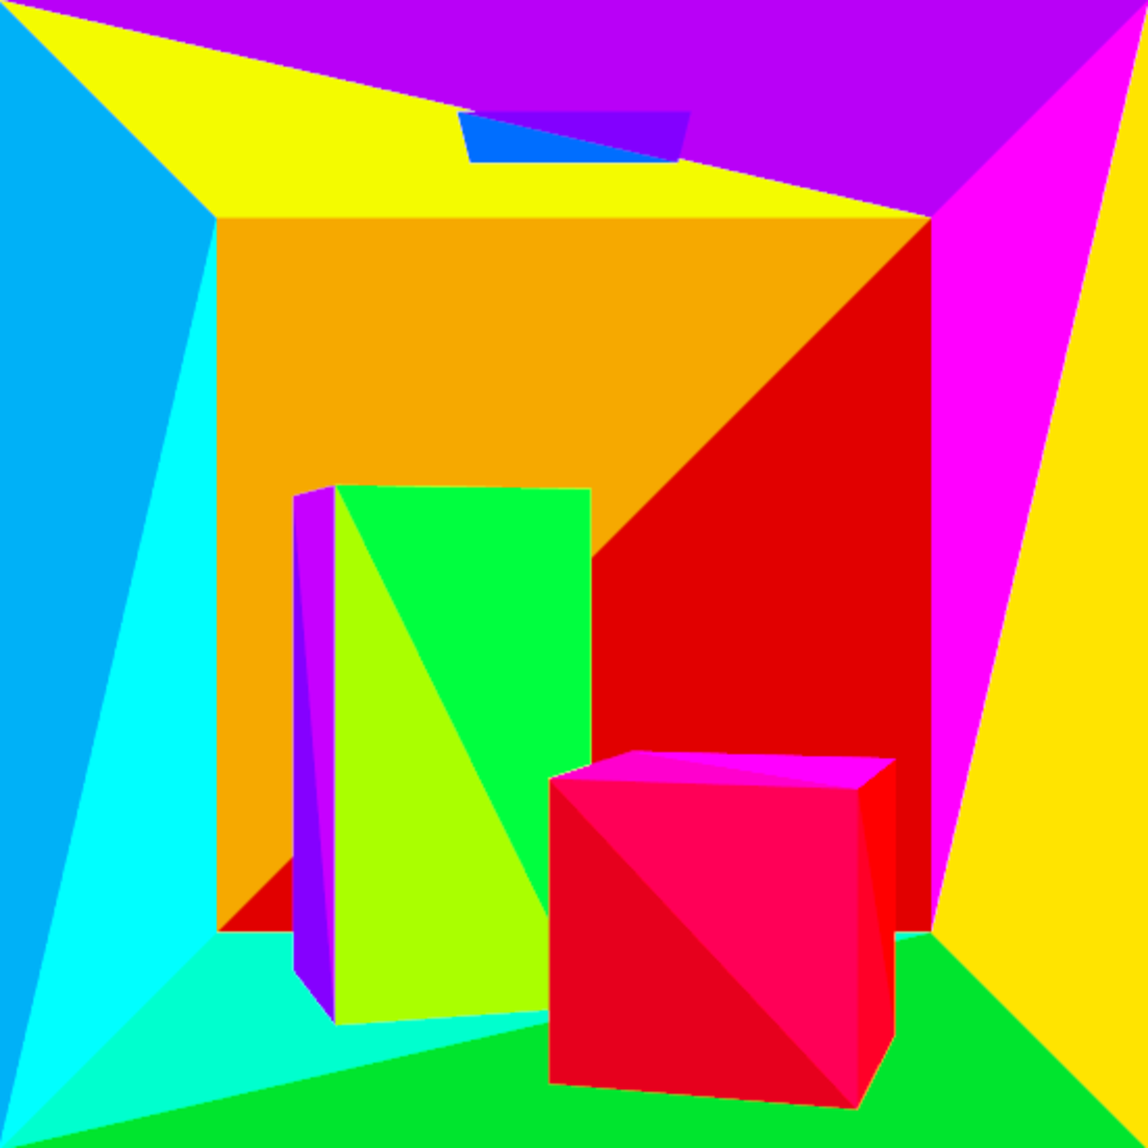
\includegraphics[width=\textwidth]{chapters/chapter_thetool/uvmap_scene}
		\caption{Scene}
	\end{subfigure}
	\begin{subfigure}[t]{0.24\linewidth}
		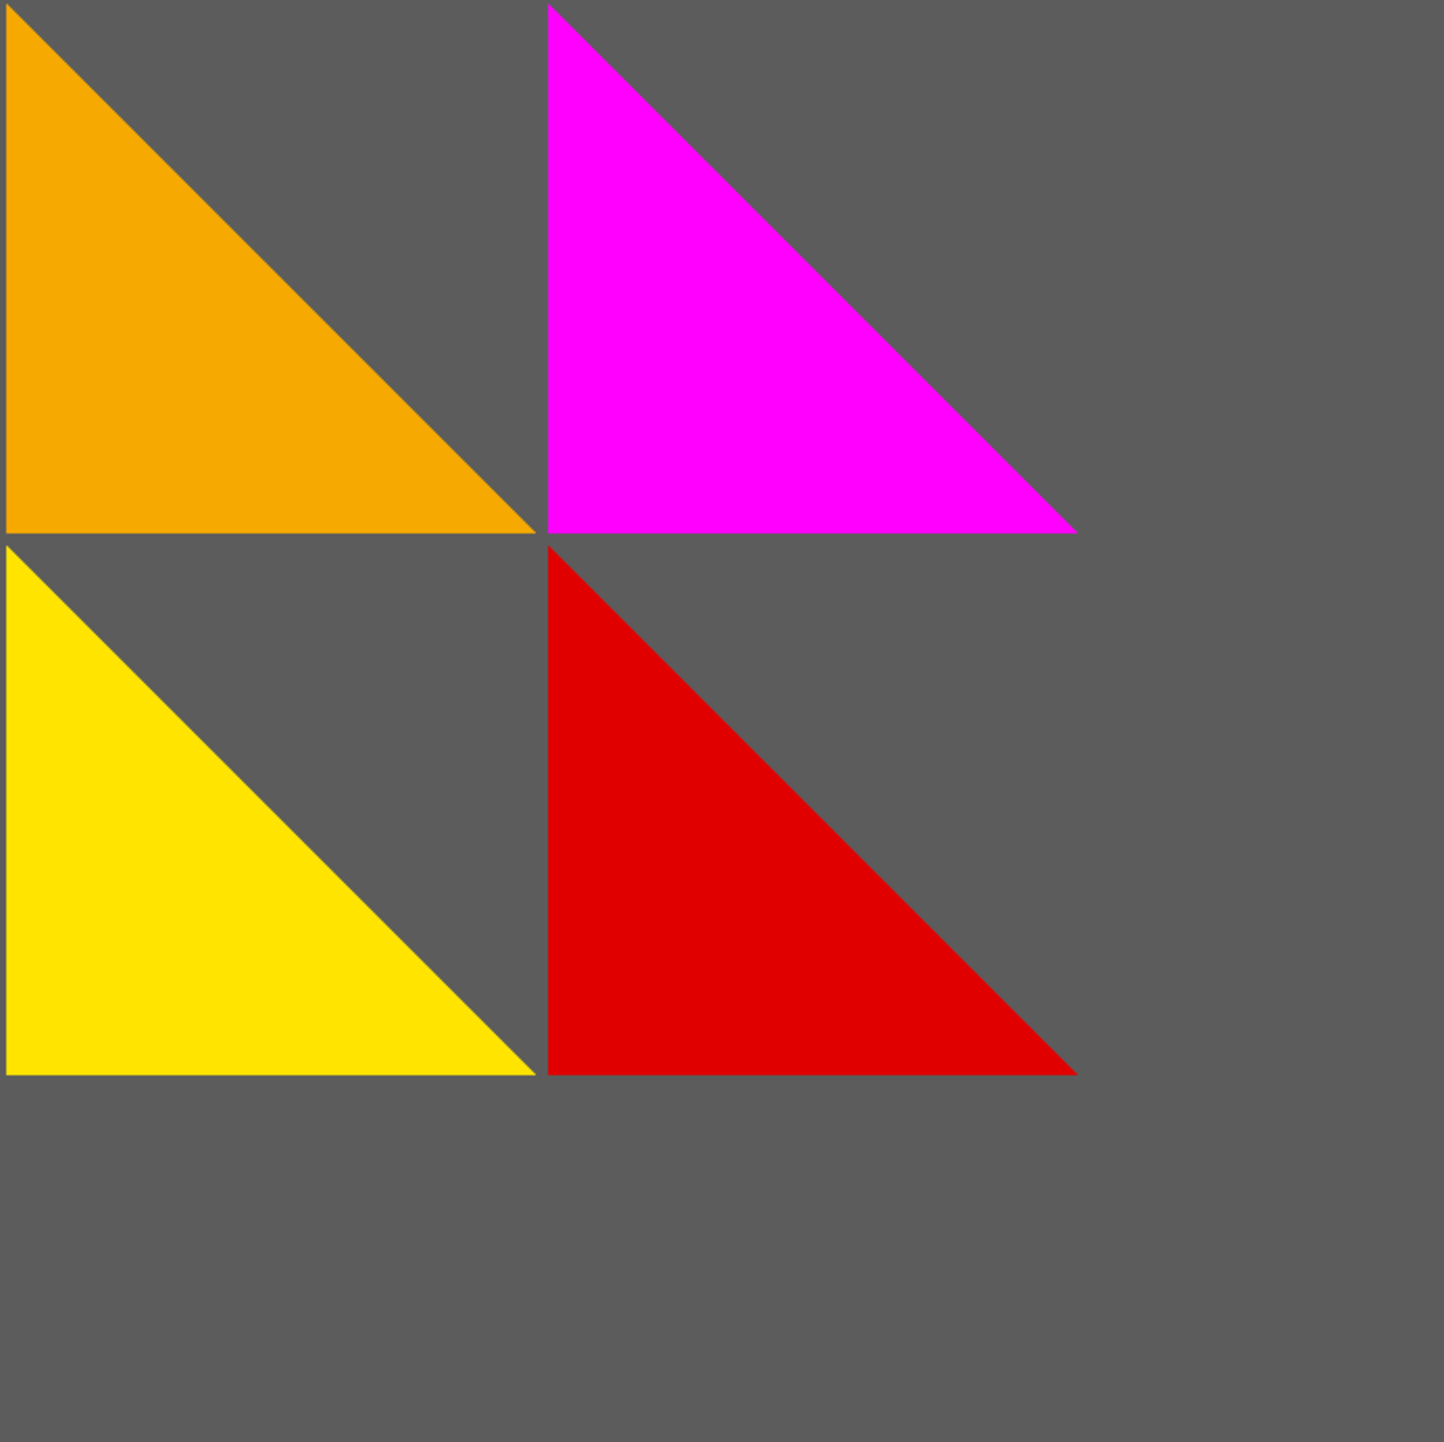
\includegraphics[width=\textwidth]{chapters/chapter_thetool/uvmap_set0}
		\caption{Map n.0}
	\end{subfigure}
	\begin{subfigure}[t]{0.24\linewidth}
		
\includegraphics[width=\textwidth]{chapters/chapter_thetool/uvmap_set1}
		\caption{Map n.1}
	\end{subfigure}
	\begin{subfigure}[t]{0.24\linewidth}
		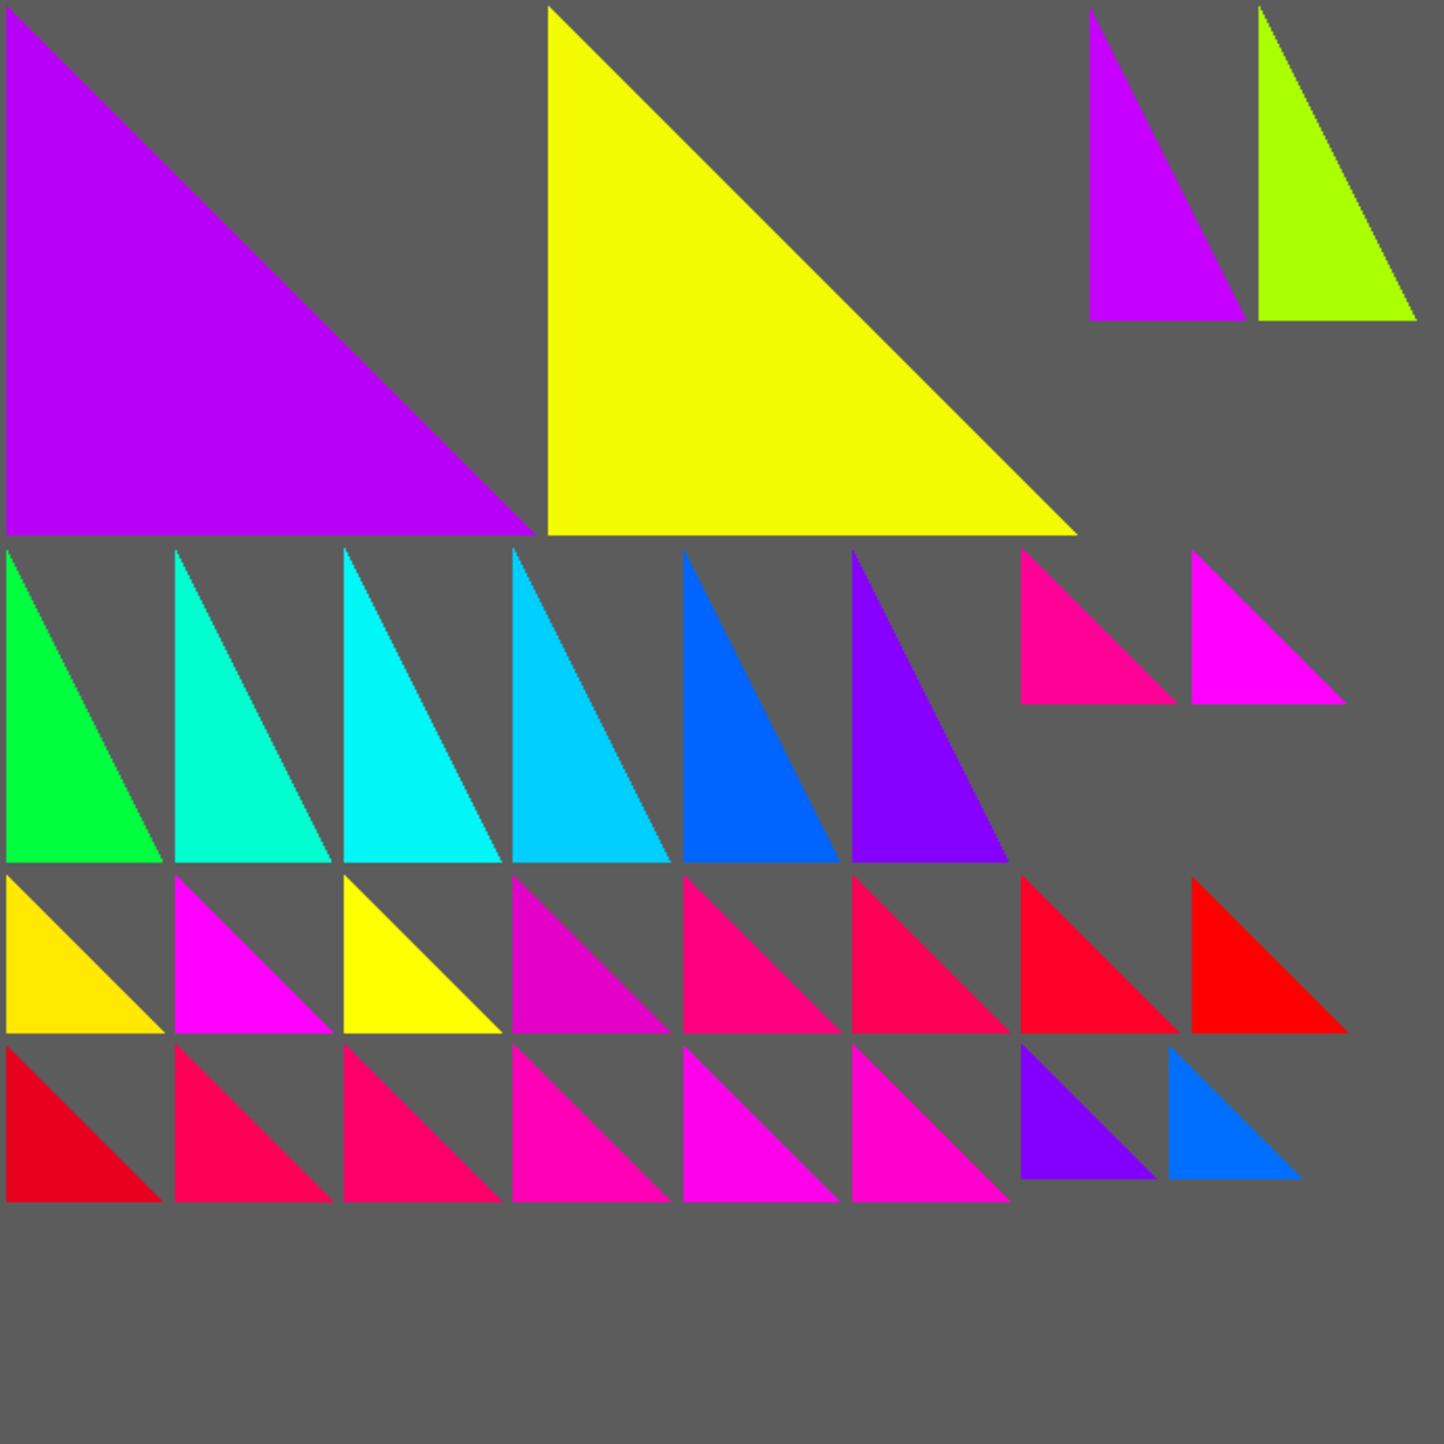
\includegraphics[width=\textwidth]{chapters/chapter_thetool/uvmap_set2}
		\caption{Map n.2}
	\end{subfigure}

	\caption{Triangles of the \textit{Cornell Box} scene rendered on the UV space. A unique color has been applied to every triangle so that it is easier to find matches between the 3D render (a) and the maps (b, c, d).}
	\label{uvmap_gen}
\end{figure}

At the end of this operation, the output is equivalent to the one visualized in figure \ref{uvmap_gen}: a 2-dimensional UV coordinate spanning across several texture squares is assigned to each scene vertex. These coordinates are appended to the vertex buffers on the GPU used for scene rendering.

\begin{figure}
	\centering
	\begin{subfigure}[t]{0.24\linewidth}
		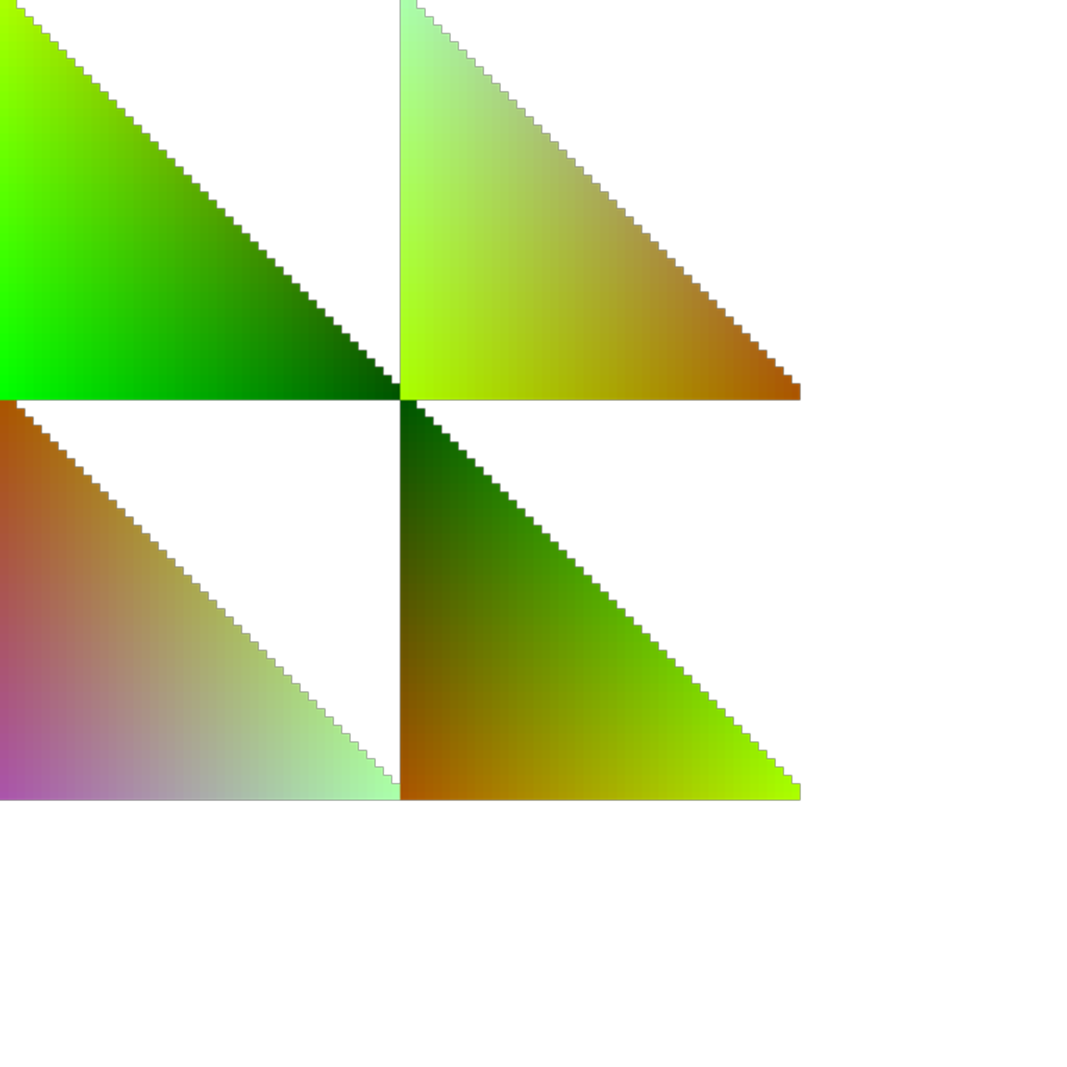
\includegraphics[width=\textwidth]{chapters/chapter_thetool/uvworld0}
		\caption{Map n.0}
	\end{subfigure}
	\begin{subfigure}[t]{0.24\linewidth}
		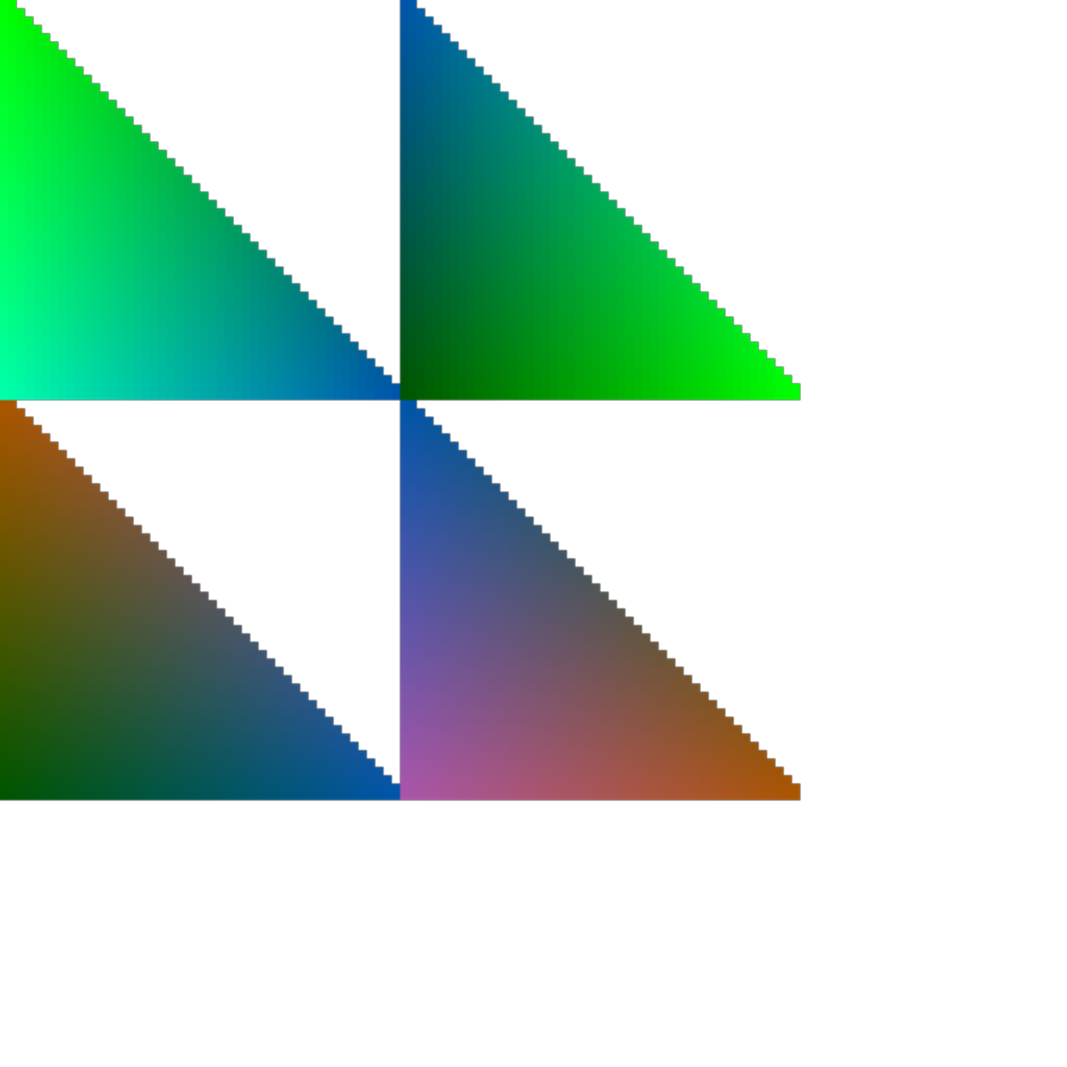
\includegraphics[width=\textwidth]{chapters/chapter_thetool/uvworld1}
		\caption{Map n.1}
	\end{subfigure}
	\begin{subfigure}[t]{0.24\linewidth}
		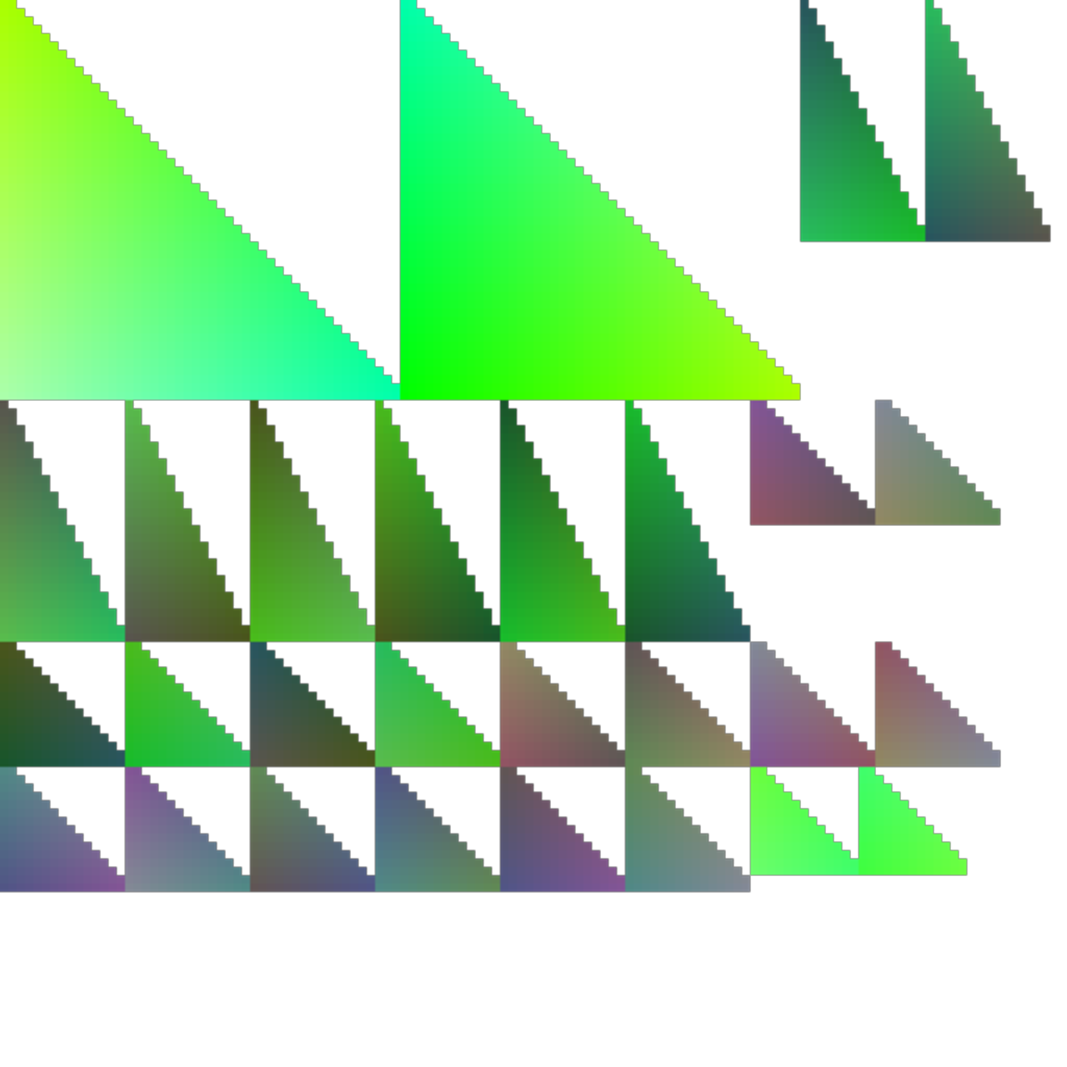
\includegraphics[width=\textwidth]{chapters/chapter_thetool/uvworld2}
		\caption{Map n.2}
	\end{subfigure}

	\caption{The world positions of the surface points of the \textit{Cornell Box} scene rendered on the UV space shown in figure \ref{uvmap_gen}. Black point has been set to $-1$ and the white one to $+2$ to improve readability.}
	\label{uvworld}
\end{figure}

Once the triangles have been arranged in the UV space, the actual heatmap has to be generated. Since our goal is to provide a heatmap showing the density of path bounces on the scene surfaces, points in world coordinates have to be compared with triangular meshes surfaces. To enable this comparison, the world coordinates of the scene triangles are rasterized onto the UV space using an ad hoc OpenGL render pipeline. The result of this operation, shown in figure \ref{uvworld}, are multiple \texttt{RGB32F} --- so that negative values are valid --- textures where each fragment holds the world coordinates of the corresponding area patch. In other words, every colored pixel of these textures corresponds to a world space point. Making these maps as precise as they can be had been proven crucial to reduce artifacts in the final heatmap renderings and that lead to extra care while designing this particular rasterization pipeline: for example, to make sure triangles narrower or even smaller than a pixel are correctly rasterized, individual triangles are rendered first as \texttt{GL\_POINTS}, then as \texttt{GL\_TRIANGLES} with the \texttt{GL\_CONSERVATIVE\_RASTERIZATION\_NV} option activated, and finally as \texttt{GL\_TRIANGLES} with \texttt{GL\_FRONT\_AND\_BACK} polygonMode set to \texttt{GL\_LINE} --- so as wireframe. These multiple steps may seem --- and they are --- rather slow but since this render pipeline is invoked only once on scene load, it results reasonable.

%TODO: insert heatmap picture

Having these \textit{UV $\to$ world mappings} and the texel size in world units at hand, computing the actual heatmap can be done by counting for each pixel the path bounces that lie within a sphere centered on the world point stored in it and having radius equal to the texel size. 
Although conceptually easy, this algorithm requires a remarkable amount of time to complete; after all, for each pixel of those textures, it has to iterate over all path bounces of the dataset. Once considered that a reasonable dataset has about half a billion bounces, it is clear that this operation takes time. This is further worsened by the impossibility of performing any kind of early termination since knowing that a bounce of a path lies within a sphere does not ensure the other bounces of the same path will not and vice versa.
To speed up the computation the obvious step of making it multi-threaded has been taken almost immediately and due to the \textit{embarrassingly parallel} nature of the algorithm, time improvements are linearly proportional to the number of available CPU cores. Even with multi-threading and further measures taken to reduce memory allocation and cache trashing, the performances are still disastrous. To give an idea, to generate a heatmap of a $512 \times 512$ pixels render with 256 spp of the \textit{Modern Hall} \cite{bitterliscenes} scene on an Intel Core i7-6820HQ (4 physical cores, 8 concurrent threads), it takes about five hours. Possible improvements were thought, most of them regarding embedding the bounces in a spatial acceleration structure, but they have never been implemented and left for future developments. At the beginning it was planned that the tool would compute heatmaps on the fly and everything was designed to accommodate that but, as soon as it was clear the times to generate one are unbearably long, the system has been coded to quietly dumps a heatmap on disk as soon as it is done computing and to load that copy the next time the same dataset is loaded. It was also thought of making the heatmap generation optional and asynchronous --- now it is blocking --- but even this never saw the light due to time constraints.

%TODO: It might be extended by letting users draw transfer maps over a histogram.


\subsection{Double dataset handling}
In the middle of development it became progressively clearer that having a way to compare two different datasets with ease would have been a crucial feature to perform debugging on datasets. To satisfy this necessity, the possibility to load two datasets at once was implemented. From the user perspective, when a second dataset is loaded, nothing changes but for the appearance of the \textbf{“Dataset switcher”} panel: every other UI component stays the same and it has the same functionalities as before but now the user can either click on the \textbf{“Switch dataset”} button or press the \textbf{X} keyboard key to switch back and forth between the two datasets. In the current status of things, when a switch happens all visualization changes but the parameters, settings, and filters chosen by the user stay the same. Extra care has been taken to make switching as fast as an ordinary frame render to allow a delay free experience of this rather critical interaction. This came to the expense of memory: both datasets have to be loaded on primary memory at all times and the same goes with the currently selected paths on the GPU memory.

% TODO: talk about possible other comparisons like a image difference

\subsection{Scene format}
\label{scene_format}

As mentioned before, this tool uses an ad hoc scene description format. This format supports only triangle meshes and represents each with one vertex and one index buffer. A whole scene is contained in a JSON \cite{rfc8259} and a binary file. They must have the same name and respectively have the \texttt{.json} and \texttt{.bin} extension. 

The binary file contains all the mesh buffers as a contiguous sequence of little-endian 32bits numbers. While vertex buffers are stored as arrays of single precision floats, index buffers are arrays of unsigned integers. 

The JSON file beside containing information about the camera and the render image, it lists the scene geometries. For each it stores a color, a flag determining if the object is in any way translucent, a name, and buffer descriptions for both the vertex and the index buffer. These have a field holding their type --- which is either \texttt{vertices} or \texttt{indices} ---, an \texttt{offset} field determining the distance in bytes from the beginning of the binary file to the first byte of the buffer, and a \texttt{size} field storing the size of the buffer in bytes. For detailed information on the JSON structure a schema is provided in Appendix \ref{json_schema}.

\begin{figure}
	\centering
	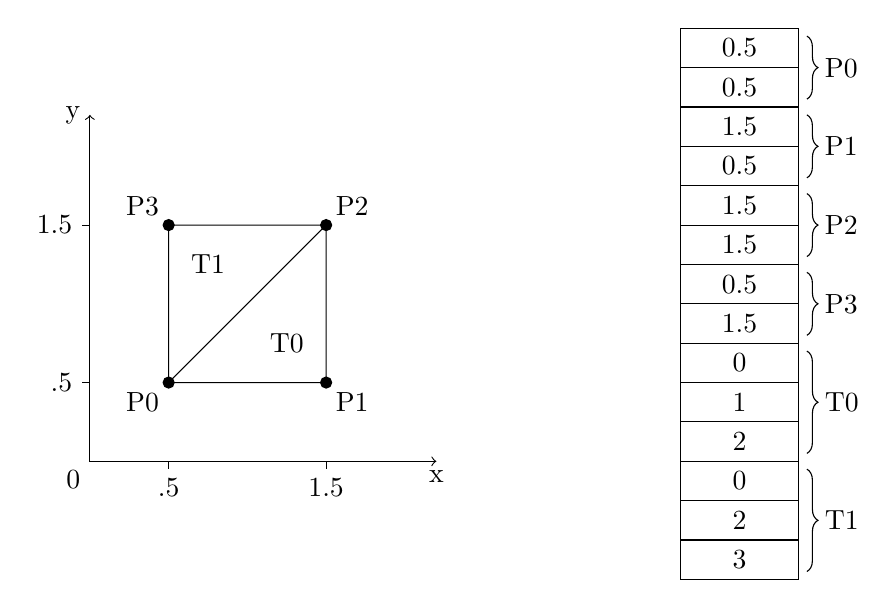
\begin{tikzpicture}
		% 2D scene
		\begin{scope}[shift={(0,0)}, scale=2]
			\draw[<->] (2.2,0) node[below]{x} -- (0,0) -- (0,2.2) node[left]{y};
			\draw (.5,0) -- (.5,-0.05) node[below]{.5};
			\draw (1.5,0) -- (1.5,-0.05) node[below]{1.5};
			\draw (0,.5) -- (-0.05,.5) node[left]{.5};
			\draw (0,1.5) -- (-0.05,1.5) node[left]{1.5};
			\begin{scope}[shift={(0.5,0.5)}]
				\draw (0,0) -- (0,1) -- (1,1) -- (0,0) -- (1,0) -- (1,1);
				\filldraw (0,0) circle (1pt) node[below left]{P0};
				\filldraw (1,0) circle (1pt) node[below right]{P1};
				\filldraw (1,1) circle (1pt) node[above right]{P2};
				\filldraw (0,1) circle (1pt) node[above left]{P3};
				\node at (.25, .75) {T1};
				\node at (.75, .25) {T0};
			\end{scope}
			\node[below left] at (0,0) {0};
		\end{scope}

		\begin{scope}[shift={(9,5.5)}, xscale=1.5, rotate=180]
			\draw (0,7) -- (0,0) -- (1,0) -- (1,7); 

			\draw (0,.5) -- (1,.5);
			\node at (.5, .25) {0.5};

			\draw (0,1) -- (1,1);
			\node at (.5, .75) {0.5};

			\draw (0,1.5) -- (1,1.5);
			\node at (.5, 1.25) {1.5};

			\draw (0,2) -- (1,2);
			\node at (.5, 1.75) {0.5};

			\draw (0,2.5) -- (1,2.5);
			\node at (.5, 2.25) {1.5};

			\draw (0,3) -- (1,3);
			\node at (.5, 2.75) {1.5};

			\draw (0,3.5) -- (1,3.5);
			\node at (.5, 3.25) {0.5};

			\draw (0,4) -- (1,4);
			\node at (.5, 3.75) {1.5};

			\draw (0,4.5) -- (1,4.5);
			\node at (.5, 4.25) {0};

			\draw (0,5) -- (1,5);
			\node at (.5, 4.75) {1};

			\draw (0,5.5) -- (1,5.5);
			\node at (.5, 5.25) {2};

			\draw (0,6) -- (1,6);
			\node at (.5, 5.75) {0};

			\draw (0,6.5) -- (1,6.5);
			\node at (.5, 6.25) {2};

			\draw (0,7) -- (1,7);
			\node at (.5, 6.75) {3};

			\draw [decorate,decoration={brace,amplitude=4pt},xshift=-2pt]
			(0,0.1) -- (0,0.9) node [right,midway,xshift=3pt]{P0};
			\draw [decorate,decoration={brace,amplitude=4pt},xshift=-2pt]
			(0,1.1) -- (0,1.9) node [right,midway,xshift=3pt]{P1};
			\draw [decorate,decoration={brace,amplitude=4pt},xshift=-2pt]
			(0,2.1) -- (0,2.9) node [right,midway,xshift=3pt]{P2};
			\draw [decorate,decoration={brace,amplitude=4pt},xshift=-2pt]
			(0,3.1) -- (0,3.9) node [right,midway,xshift=3pt]{P3};

			\draw [decorate,decoration={brace,amplitude=4pt},xshift=-2pt]
			(0,4.1) -- (0,5.4) node [right,midway,xshift=3pt]{T0};
			\draw [decorate,decoration={brace,amplitude=4pt},xshift=-2pt]
			(0,5.6) -- (0,6.9) node [right,midway,xshift=3pt]{T1};
		\end{scope}
	\end{tikzpicture}

	\caption{Geometry example. To simplify, a 2-dimensional case is presented. On the right a simple triangulated mesh is shown, on the left there is a valid binary file. A corresponding JSON file is shown in Listing \ref{scene_json}.}
	\label{scene_bin}
\end{figure}

\begin{Listing}
	\begin{lstlisting}
{
	"camera": {...},
	"render": {...},
	"geometries": [
		{
			"name":     "quad",
			"material": {...},
			"buffers": [
				{
					"offset": 0,
					"size":   32,
					"type":   "vertices"
				},
				{
				 	"offset": 32,
				 	"size":   24,
				 	"type":   "indices"
				}
			]
		}
	]
}
	\end{lstlisting}
	\caption{JSON scene file example relative to Figure \ref{scene_bin}. Information not relative to the geometry shape has been omitted. Please also remember this is a 2-dimensional example, hence the vertex buffer size is only 2 dimensions * 4 points * 4 bytes = 32 bytes instead of being 48 bytes like it would be in the ordinary 3-dimensional case.}
	\label{scene_json}
\end{Listing}